\documentclass[14pt,a4paper,oldfontcommands]{memoir}
\usepackage{amsmath}
\usepackage[utf8]{inputenc}
\usepackage[T1]{fontenc}
\usepackage{microtype}
\usepackage[dvips]{graphicx}
\usepackage{xcolor}
\usepackage{times}
\usepackage{mathrsfs}
\usepackage[
breaklinks=true,colorlinks=true,
%linkcolor=blue,urlcolor=blue,citecolor=blue,% PDF VIEW
linkcolor=black,urlcolor=black,citecolor=black,% PRINT
bookmarks=true,bookmarksopenlevel=2]{hyperref}

\usepackage{geometry}
% PDF VIEW
% \geometry{total={210mm,297mm},
% left=25mm,right=25mm,%
% bindingoffset=0mm, top=25mm,bottom=25mm}
% PRINT
\geometry{total={276mm,297mm},
left=25mm,right=25mm,
bindingoffset=10mm, top=25mm,bottom=25mm}

\OnehalfSpacing
%\linespread{1.3}

%%% CHAPTER'S STYLE
%%%%%%\chapterstyle{bianchi}
%\chapterstyle{ger}
%\chapterstyle{madsen}
%\chapterstyle{ell}
%%% STYLE OF SECTIONS, SUBSECTIONS, AND SUBSUBSECTIONS
%%%%%%\setsecheadstyle{\Large\bfseries\sffamily\raggedright}
%%%%%%\\setsubsecheadstyle{\large\bfseries\sffamily\raggedright}
%%%%%%\\setsubsubsecheadstyle{\bfseries\sffamily\raggedright}


%%% STYLE OF PAGES NUMBERING
%\pagestyle{companion}\nouppercaseheads 
%\pagestyle{headings}
%\pagestyle{Ruled}
\pagestyle{plain}
\makepagestyle{plain}
\makeevenfoot{plain}{\thepage}{}{}
\makeoddfoot{plain}{}{}{\thepage}
\makeevenhead{plain}{}{}{}
\makeoddhead{plain}{}{}{}


\maxsecnumdepth{subsection} % chapters, sections, and subsections are numbered
\maxtocdepth{subsection} % chapters, sections, and subsections are in the Table of Contents


%%%---%%%---%%%---%%%---%%%---%%%---%%%---%%%---%%%---%%%---%%%---%%%---%%%

\begin{document}

%%%---%%%---%%%---%%%---%%%---%%%---%%%---%%%---%%%---%%%---%%%---%%%---%%%
%   TITLEPAGE
%
%   due to variety of titlepage schemes it is probably better to make titlepage manually
%
%%%---%%%---%%%---%%%---%%%---%%%---%%%---%%%---%%%---%%%---%%%---%%%---%%%
\thispagestyle{empty}

{%%%
%%%%%%\\sffamily
\centering
\Large

~\vspace{\fill}

\textbf{\huge 
Search for new ZZ resonances in two leptons two neutrinos final states at 13 TeV using 2016 CMS dataset
}

\vspace{0.5cm}

{\LARGE
Yanchu Wang\\
}
Charlottesville, VA\\[1em]

B.S., University of Science and Technology of China, 2013

\vspace{1.5cm}
Advisor: Prof. Robert Hirosky\\[1em]
\vspace{2.5cm}
\vspace{\fill}
\textrm{\textit{A Thesis presented to the Graduate Faculty of the University of Virginia in Candidacy for the Degree of Doctor of Philosophy}}

\vspace{2.5cm}


\vspace{\fill}
Department of Physics\\[1em]
University of Virginia\\
May, 2018

%%%
}%%%

\cleardoublepage
%%%---%%%---%%%---%%%---%%%---%%%---%%%---%%%---%%%---%%%---%%%---%%%---%%%
%%%---%%%---%%%---%%%---%%%---%%%---%%%---%%%---%%%---%%%---%%%---%%%---%%%
\begin{center}
\textbf{\huge ACKNOWLEDGEMENT}
\end{center}
\vspace{0.5cm}

First and foremost, I would like to express my immerse gratitude to my advisor Prof. Bob Hirosky, for his continual guidance and support throughout the last 4 years for me. He guided me into the world of experimental particle physics and fascinated me with his physics insight and technical skills. 

\vspace{0.3cm}
I would also like to express my gratitude to Dr. Hengne Li, the former post-doctor in our group who now works as a professor at the South China Normal University. His dedication to research has always been an invaluable source of inspiration to me. 

\vspace{0.3cm}
Moreover, I appreciate the efforts from the members of my defense committee, including Dr. Brad Cox, Dr. P.Q. Hung and Dr. Nitya Kallivayalil, for their time reviewing my research, providing precious comments for my thesis, and approving my dissertation.

\vspace{0.3cm}
In addition, I am grateful to the physicists I worked with and learnt from during my 2 years' stay at CERN, such as Tote Hughes and Andrew Whitbeck in the HCAL Phase I upgrading team, Mario Galanti and Josh Kunkle in the HCAL Operation team, Thomas Peiffer and Vieri Candelise in the B2G MC Production team, and many more amazing researchers in the collaboration. 

\vspace{0.3cm}
Finally, I could not have achieved this without the encouragement and love from my parents. I am grateful to my mother Cailing Hu and father Zhiping Wang for supporting me along the way.
\vspace{0.5cm}
\begin{flushleft}
Yanchu Wang

Charlottesville, VA

April, 2019
\end{flushleft}
\newpage

\clearpage
\begin{center}
\textbf{\huge Preface}
\end{center}
\begin{flushright}
\Large{--- CMS and me}
\end{flushright}
\vspace{0.5cm}
In August 2014, I joined the UVA CMS group and worked on calibrating a prototype Shashlik calorimeter using the muon data as my first project here. Afterwards, in the middle of 2015, I left for CERN, Switzerland and stayed there for 2 years. During my stay at CERN I was involved in several projects and activities both on the detector and physics analysis. 

\vspace{0.3cm}
My most detector-related work focused on the Hadron Calorimeter (HCAL). Starting with the Hadron Forward (HF) detector frontend electronics Phase I upgrade in 2015, I joined the HCAL upgrade team, helping design and carry out a series of electronics tests. In 2016 I helped the HCAL Endcap (HE) upgrade with system monitoring and the HCAL Data Quality Management (DQM) group with their online DQM system for the HF/HE upgrades. I was also taking HCAL detector on call expert shifts continually for 1 year and a half since 2016.

\vspace{0.3cm}
In terms of physics analysis, I started working on this di-boson analysis~\cite{thispaper} in the December of 2015, helping to design and implement the analysis framework from scratch, studying the pileup reweighting, trigger efficiency, lepton identification algorithms and their efficiencies, as well as determining the non-resonant background using data-driven modeling. The muon tracker High $p_{T}$ efficiency calculated by me has been widely used in related CMS analyses and I am also contributing to the high $p_{T}$ muon paper carried out by the muon Physics Object Group (POG). Apart from this di-boson analysis, I also worked as the Monte Carlo/Generator contact person for physics simulations in the Beyond Two Generations (B2G) Physics Analysis Group (PAG) for the whole year of 2017.

\clearpage
\tableofcontents*

\clearpage

%%%---%%%---%%%---%%%---%%%---%%%---%%%---%%%---%%%---%%%---%%%---%%%---%%%
%%%---%%%---%%%---%%%---%%%---%%%---%%%---%%%---%%%---%%%---%%%---%%%---%%%

\chapter{Introduction}

\section{The Standard Model}
The Standard Model (SM)\cite{SMref1,SMref2,SMref3} is the fundamental theory of elementary particle physics. After half a century's development, the Standard Model framework has been confirmed by numerous experiments and can be used to explain most of the data collected about interactions of the fundamental particles. In the Standard Model there are generally 2 categories of particles: fermions and bosons. Fermions, which always have half-integer spins, make up all the matter in the universe. On the other hand, bosons with integer spins mediate the fundamental interactions among the fermions, and the interactions here include the electro-magnetic interaction, the weak interaction and the strong interaction. Figure~\ref{fig:smpfamily} shows all the particles that have been discovered and included in the Standard Model.
\begin{figure}[htbp]
\begin{center}
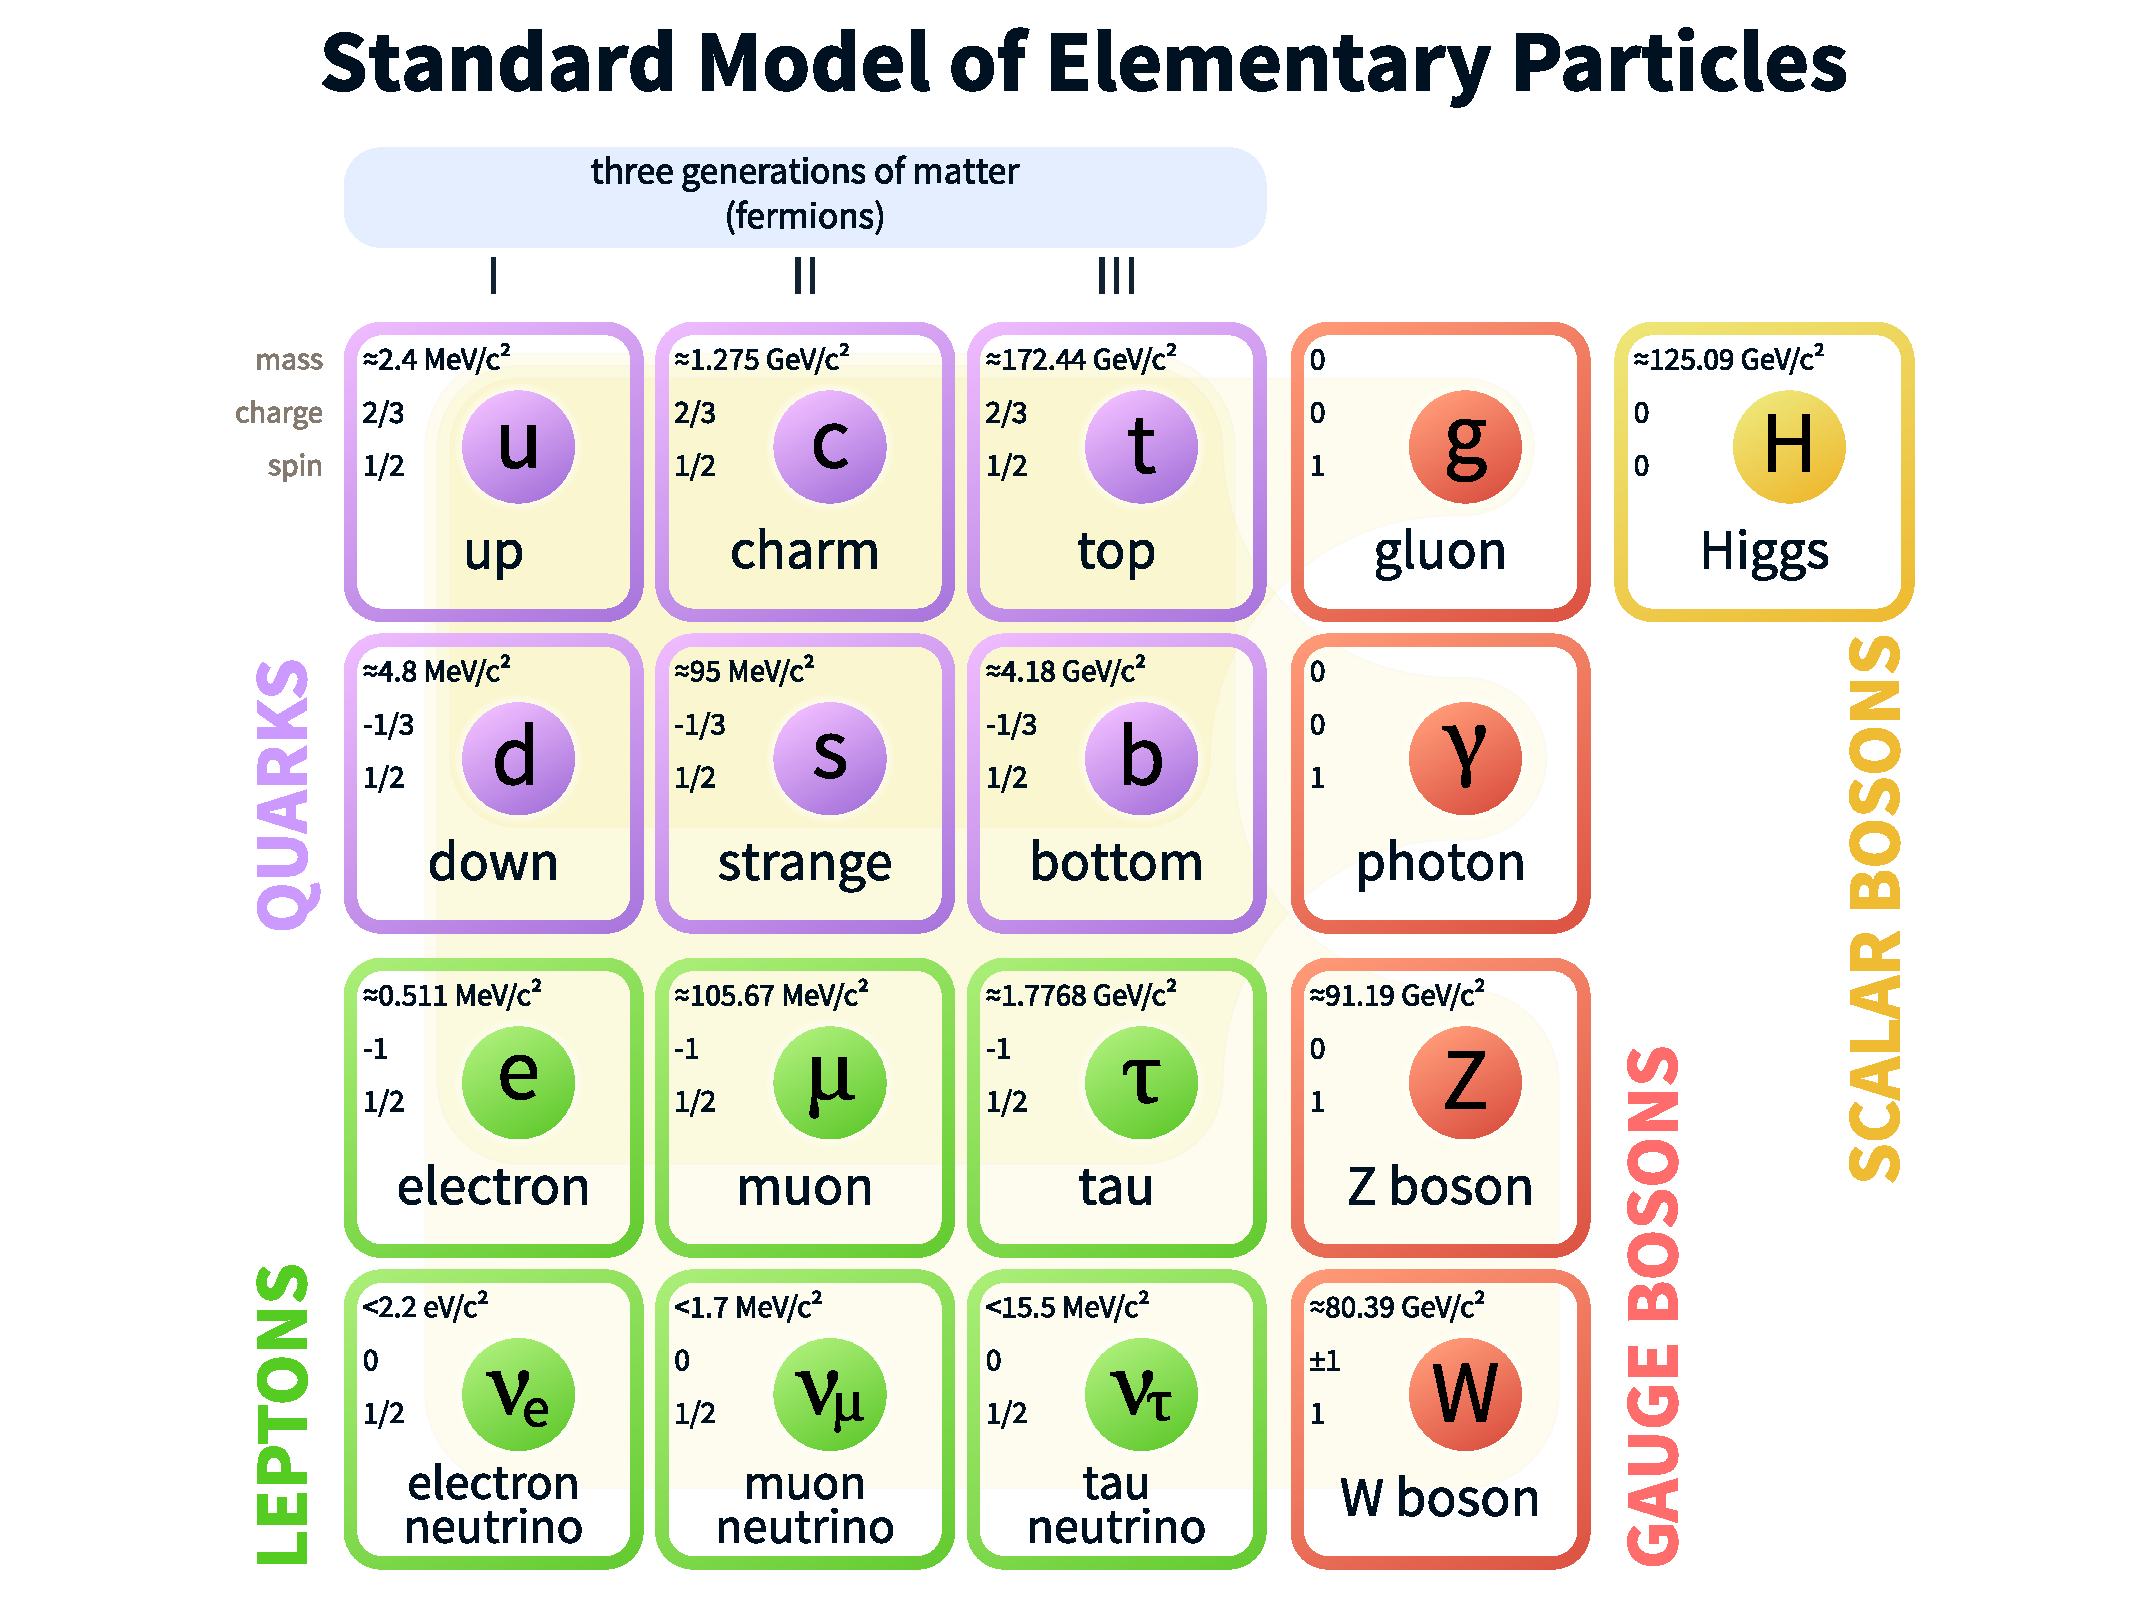
\includegraphics[width=0.72\linewidth]{figures/smpfamily.pdf}
\caption{The Standard Model contains 3 generations of leptons and quarks, 4 kinds of vector bosons and the Higgs boson.}
\label{fig:smpfamily}
\end{center}
\end{figure}

\subsection{Fermions}
Fermions are particles that follow Fermi–Dirac statistics and obey the Pauli exclusion principle. Every fermion has its anti particle, which is a fermion with opposite charge but same mass and spin. The elementary fermions in the Standard Model include leptons and quarks, both of them consist of 3 generations and each generation consists of 2 flavors of fermions. Every elementary fermion in the Standard Model has a spin of one half.
\subsubsection{Lepton}
The leptons do not participate in the strong interaction. There are 3 generations of leptons, and each generation consists of two flavors of leptons: one charged lepton, and one neutral lepton also known as a "neutrino". The charged lepton always carries 1 unit of elementary electric charge, negative for a lepton and positive for its anti-lepton. The masses of the charged leptons have been precisely measured as shown in Figure~\ref{fig:smpfamily}. In the SM, neutrinos are regarded to be massless.

\vspace{0.3cm}
The first generation of leptons includes the electron ($e^{-}$) and electron-neutrino ($\nu _{e}$). Both electron and electron-neutrino have an electron number $L_{e}=1$, while their anti leptons have $L_{e}=-1$. The second generation leptons, the muon ($\mu$) and muon-neutrino ($\nu_{\mu}$), have a muon number $L_{\mu}=1$, while $L_{\mu }=-1$ for the anti-muon ($\bar{\mu}$) and anti-muon-neutrino ($\bar{\nu} _{\mu }$). Similarly, the third generation consists of the tau ($\tau$) and tau-neutrino ($\nu _{\tau }$), with a tau number $L_{\tau}$ accordingly.

\vspace{0.3cm}
In the SM, under the assumption that neutrinos are massless, the lepton numbers are strictly conserved in any kind of interaction. However, recent experiments~\cite{neutrinoOscillation1,neutrinoOscillation2} indicate that the neutrinos have small masses, which implies the lepton numbers can be mixed among different generations.
\subsubsection{Quark}
A quark can participate in any of the 3 interactions in the Standard Model. Like leptons, quarks fall into 3 generations, and each generation contains 2 flavors of quarks having 2/3 and -1/3 elementary electric charge correspondingly. Besides electric charge, quarks also have another intrinsic property known as color charge. The color charge a quark carries is typically defined to be red, blue or green, while the anti quark carries a corresponding anti-color. Quarks are never observed directly in an isolated state due to the phenomenon of color confinement, which confines quarks to only exist in composite, colorless particles known as hadrons.

\vspace{0.3cm}
The first generation includes up and down quarks, the second generation includes charm and strange quarks, and the third generation consists of top and bottom quarks. Every quark has its anti quark, with opposite charge. The mass for each quark is shown in Figure~\ref{fig:smpfamily}. It is possible for heavier quarks to decay into lighter quarks through the weak interaction, especially for quarks within the same generation.
\subsection{Bosons and the interactions}
In contrast to fermions, bosons are particles that follow Bose–Einstein statistics allowing multiple particles in the same state. In the SM there are 4 kinds of vector bosons each with spin 1 and one spin-0 scalar boson, which is the recently discovered Higgs boson. The vector bosons work as force carriers of the 3 interactions, while the masses of the elementary particles are generated by their interaction with the Higgs field.
\subsubsection{Vector Bosons}
In the SM, the vector bosons (gluon, photon, Z boson and W boson) work as mediators of the 3 fundamental interactions among fermions. Each of the vector bosons has spin 1.
\begin{itemize}
\item the \textbf{gluon} is the force mediator of the strong interaction, described in Quantum Chromodynamics (QCD) theory, a gauge theory based on SU(3). Gluons are massless and have no electric charge.
\item the \textbf{photon} is the force mediator of the electromagnetic interaction, described in Quantum Electrodynamics (QED) theory, a $U(1)_{EM}$ theory. Photons are massless and have no electric charge.
\item the \textbf{Z boson} is the mediator of the weak interaction with no electric charge flow. The Z boson has no charge, while it has mass of 91.2\GeV, which makes it possible to decay into a fermion–antifermion pair.
\item the \textbf{W boson} is the mediator of the weak interaction with electric charge flow. The W carries either 1 or -1 elementary electric charge, denoted as $W^{+}$ and $W^{-}$, both having masses of 80.4\GeV. Like the Z boson, W bosons can decay into fermion–antifermion pairs.
\end{itemize}
In the SM, the unification of the electromagnetic and weak interactions is realized by an SU(2) $\times$ U(1) gauge group. The photon, Z boson and W boson are generated in the SU(2) $\times$ U(1) group due to the process of spontaneous symmetry breaking described by the Higgs mechanism. 
\subsubsection{The Higgs Boson}
In the 1960s the Higgs boson and Higgs mechanism was proposed in order to explain the source of the masses of the gauge bosons\cite{higgstheory1,higgstheory2,higgstheory3}, which are expected to be massless according to the gauge theory. That assumption clearly conflicts with the experiment facts. The Higgs mechanism suggests that an SU(2) doublet of complex scalar fields breaks the SU(2) symmetry as its potential in the form of $\mu^{2}\phi^{\dagger}\phi + \lambda^{2}(\phi^{\dagger}\phi)^2$ with $\mu^{2}<0$ and $\lambda^{2}>0$ leads to a non-zero vacuum expectation value which does not follow the SU(2) symmetry. This phenomenon is referred to as "spontaneous symmetry breaking" and the field here is the Higgs field. Due to the spontaneous symmetry breaking, three gauge bosons gain masses when interacting with the scalar field, and the Higgs Boson comes from one degree of freedom of the field while the other 3 degrees are no longer observable.

\vspace{0.3cm}
On July 4 of 2012, the discovery of the Higgs boson was announced by both the CMS and ATLAS Collaborations at the CERN, LHC\cite{higgsdiscover1,higgsdiscover2}. Hence the Higgs boson officially became one member of the standard model elementary particle family. The Higgs boson has no spin or electric charge, and its mass is measured to be 125\GeV. It is very unstable and mainly decays into a $b\bar{b}$ quark pair, $\tau\bar{\tau}$ pair or off shell gauge boson pair.

\section{The Limitations of SM and the Hierarchy Problem}
Although the SM has been tested and demonstrated as a great success among numerous particle physics experiments and provides reliable physics predictions for most of the sceneries, it is not yet believed to be a complete theory. The SM does not provide theoretical support for either dark energy or dark matter particles which are believed to exist according to cosmological observations. Moreover, within the SM particles, neutrino oscillation proved by several experiments conflicts with the SM's assumption of massless neutrinos. Above all, as mentioned above, the SM incorporates only 3 of the 4 fundamental interactions, leaving gravitation completely unexplained in the scope of particle physics.

\vspace{0.3cm}
The Hierarchy Problem~\cite{intro_hierarchy} in particle physics refers to the huge discrepancy between the electroweak scale and the gravitational scale, as the weak force is about $10^{24}$ times stronger than gravity. The Fermi's constant denoting the scale of the weak interaction is expected to be larger and closer to the Newton's constant for gravity, based on the calculation of SM. In other words, we expect the large quantum contributions to the square of the Higgs boson mass would make the Higgs boson much heavier than the measured 125\GeV. It could be that the measured Higgs boson mass is the result of incredibly fine-tuned constants within the SM. Alternatively, some new theoretical mechanism is expected. The Bulk RS Graviton Model is one of the possible solutions.

\section{Bulk RS Graviton Model}
The Bulk RS Graviton model offers an efficient solution to the Hierarchy problem. It also provides theoretical support for the production of heavy di-boson resonances, which can result from interactions involving an extra spatial dimension. The development and features of this model are summarized below.
\subsection{Introduction of Extra Dimension Models}
In the 1920s, the Kaluza–Klein theory was proposed as a means to unify gravitation and electromagnetism. It assumed a 5th dimension beyond our usual four dimension of space and time and started purely from the 5 dimensional extension of General Relativity. The quantum mechanical interpretation predicts that gravitons or other particles in the extra dimension will acquire quantized excited modes, which are referred to as Kaluza-Klein (K-K) modes. The K-K theory is considered an important precursor to subsequent theories that introduce extra spatial dimensions as a solution to the Hierarchy Problem.

\vspace{0.3cm}
Following the K-K theory, a number of extra dimension theories were proposed attempting to address the Hierarchy problem, such as the ADD model. The ADD model~\cite{Intro_ADD,Intro_ADD2} was proposed in 1998 by Nima Arkani-Hamed, Savas Dimopoulos, and Gia Dvali, suggesting the existence of additional large extra spatial dimensions. It proposed that the Planck scale $M_{Pl}(\sim{G_{N}}^{-1/2})$ is not a fundamental scale but is instead simply a consequence of the large size of the new dimensions. While gravitons can freely propagate in the new dimensions, at sub-weak energies the SM fields must be localized to a 4-dimensional manifold of weak scale thickness in the extra dimensions. 

\subsection{Randall–Sundrum Model}
The Randall-Sundrum (RS) model~\cite{Intro_RS1} was originally proposed in 1999 by Lisa Randall and Raman Sundrum, because they were not satisfied with those large extra dimension models that involved fine tunings of the bulk cosmological constant and brane tensions. This theory is often referred to as the RS1 model. The framework is based on a slice of 5-dimensional anti-de Sitter space ($AdS_{5}$), with two flat four-dimension branes on each boundary. According to the $AdS_{5}$ theory, if the flat 4D branes carry energy, the geometry of the additional dimension has to be warped to be consistent with the General Relativity. The line segment ($ds$) which determines the distance scale is given by equation~\ref{eqn:intro_ds},
\begin{equation}
ds^2 = e^{-2ky}{\eta}_{\mu\nu}{dx}^{\mu}{dx}^{\nu}+dy^2,
\label{eqn:intro_ds}
\end{equation}
where ${\eta}_{\mu\nu}$ is the Minkowski metric for flat four-dimension space; ${dx}^{\mu}$ is the regular time-space four-vector; $y$ represents the 5th dimension coordinate, bounded by $0\leq y \leq \pi R$ and $R$ is the extra dimension length; $k$ is the curvature constant.

\vspace{0.3cm}
Fluctuations on 2 of the variables are possible, $k$ and $R$, each corresponding to a particle field: the graviton and radion. In the RS1 model, the SM particles are all trapped on one of the branes, referred to as the TeV Brane, located at $y=\pi R$. The other brane in this model, named the Plank Brane and located at $y=0$, has a Planckian fundamental scale and is the brane where the 4D (or zero-mode) graviton concentrates. Given this assumption, it is possible to unify the fundamental gravitational and weak mass scales, since the 4D physical masses on the TeV brane acquire an exponential rescaling of $e^{-2ky}$. Figure~\ref{fig:intro_branes} gives the idea of this extra dimension model and the metric behavior.
\begin{figure}[htbp]
\begin{center}
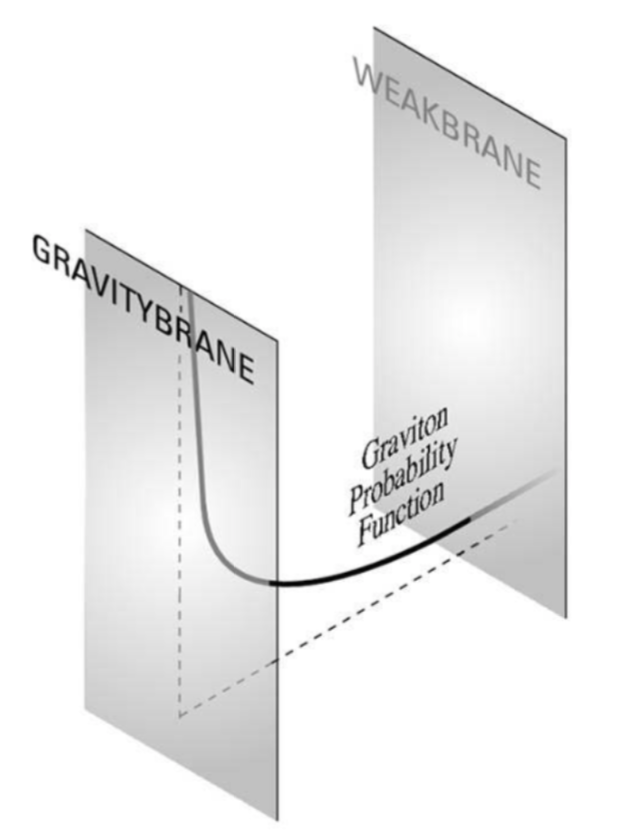
\includegraphics[width=0.32\linewidth]{figures/intro_branes.png}
\caption{In RS theory, the Gravity Brane (Planck Brane) and the Weak Brane (TeV Brane) are the 4 dimensional boundaries of the extra dimension. The metric behavior along the extra dimension is also shown.}
\label{fig:intro_branes}
\end{center}
\end{figure}

The key feature of the RS1 model is that, though the zero-mode spin-2 graviton is localized in the Plank Brane, its K-K excited mode (K-K graviton) is localized near the TeV brane and has mass around a TeV, so that K-K graviton coupling to the entire SM is only $\sim$ TeV suppressed.
\subsection{The Bulk RS Graviton Model}
However, in the RS1 model, the higher-dimensional operators in the 5D effective field theory are suppressed only by the warped scale $\sim$ TeV, giving contributions that are too large to flavor-changing neutral current (FCNC) processes~\cite{intro_rsfcnc1,intro_rsfcnc2} which are strongly suppressed in the SM.

\vspace{0.3cm}
A solution to this issue is to allow the SM fields to propagate in the extra dimension, which leads to the scenario of the Bulk RS Graviton model~\cite{intro_bulkref1,intro_bulkref2,intro_bulkref3}. In this model, the SM particles are identified with the zero-modes of the 5D fields and the profile of a SM fermion in the extra dimension depends on its 5D mass parameter. We can then choose to localize 1st and 2nd generation fermions near the Planck brane, so that their interactions to the K-K gauge bosons are suppressed, as the K-K gauge bosons are near the TeV brane and have little overlapping with the light fermions. Therefore,  the FCNCs from higher-dimensional operators are suppressed by scales far beyond TeV scale.

\vspace{0.3cm}
Like the RS1 model, the K-K gravitons are localized near the TeV brane. Figure~\ref{fig:intro_rsandbulk} shows the zero-modes of the SM matter fields and the K-K graviton along the 5th dimension, for the Bulk RS model and RS1 model.
\begin{figure}[htbp]
\begin{center}
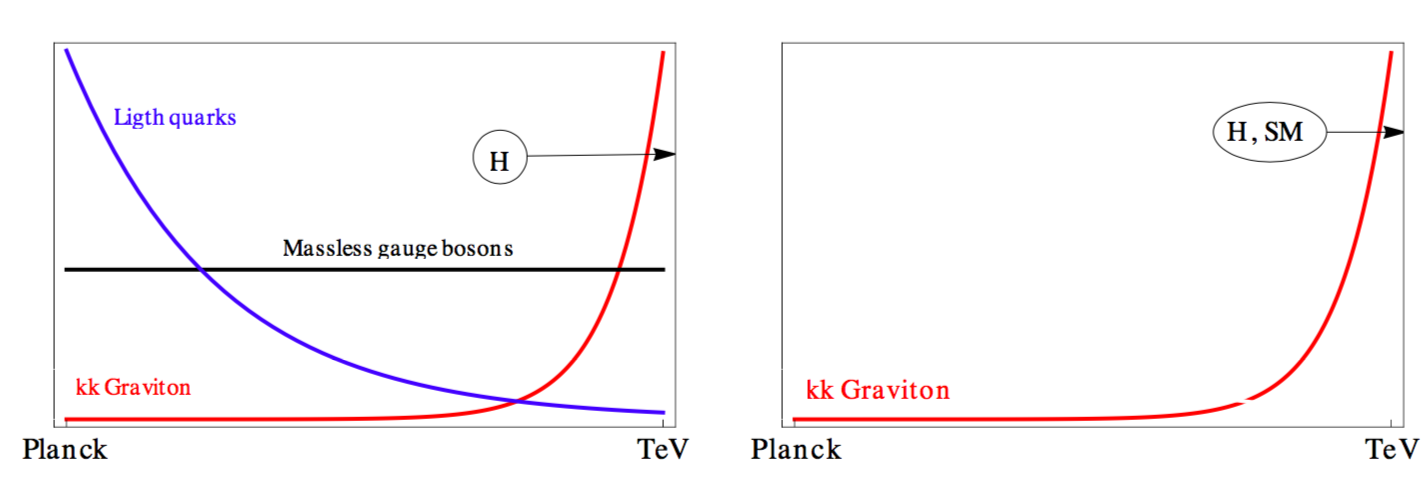
\includegraphics[width=0.9\linewidth]{figures/intro_rsandbulk.png}
\caption{Zero-modes of the SM matter fields and the K-K graviton along the extra dimension for the Bulk RS model scenario (left), and RS1 (right).}
\label{fig:intro_rsandbulk}
\end{center}
\end{figure}

From Figure~\ref{fig:intro_rsandbulk} one can see that in the Bulk RS scenario the light fermions are localized near the Plank brane while the K-K gravitons are near the TeV brane, as a result, the couplings of the K-K gravitons to light fermions are highly suppressed compared to the RS1 model. Additionally, the SM massless gauge bosons have flat distribution across the extra dimension, which also leads to the suppression of their couplings to the K-K gravitons by roughly a factor of $k\pi R$.

\subsection{Phenomenology of the Bulk Graviton Model}
As in the RS1 model, there are 2 free parameters in the RS Bulk theory, the curvature constant $k$ and the extra dimension length $R$. Equivalently they can be expressed as $\tilde{k}$, which is defined as the ratio of $k$ and the reduced Plank mass ($\overline{M_{Pl}}\equiv M_{Pl}/\sqrt{8\pi}$), and the K-K graviton mass ($m_{G}$). The K-K Graviton in the Bulk Graviton model can be produced in several ways, while the dominant process is QCD gluon fusion. Figure~\ref{fig:intro_Gxsec} shows the cross sections for the production of a Bulk Graviton production for different processes, with $\tilde{k}=0.1$ and proton-proton center of mass energy of 13TeV.
\begin{figure}[htbp]
\begin{center}
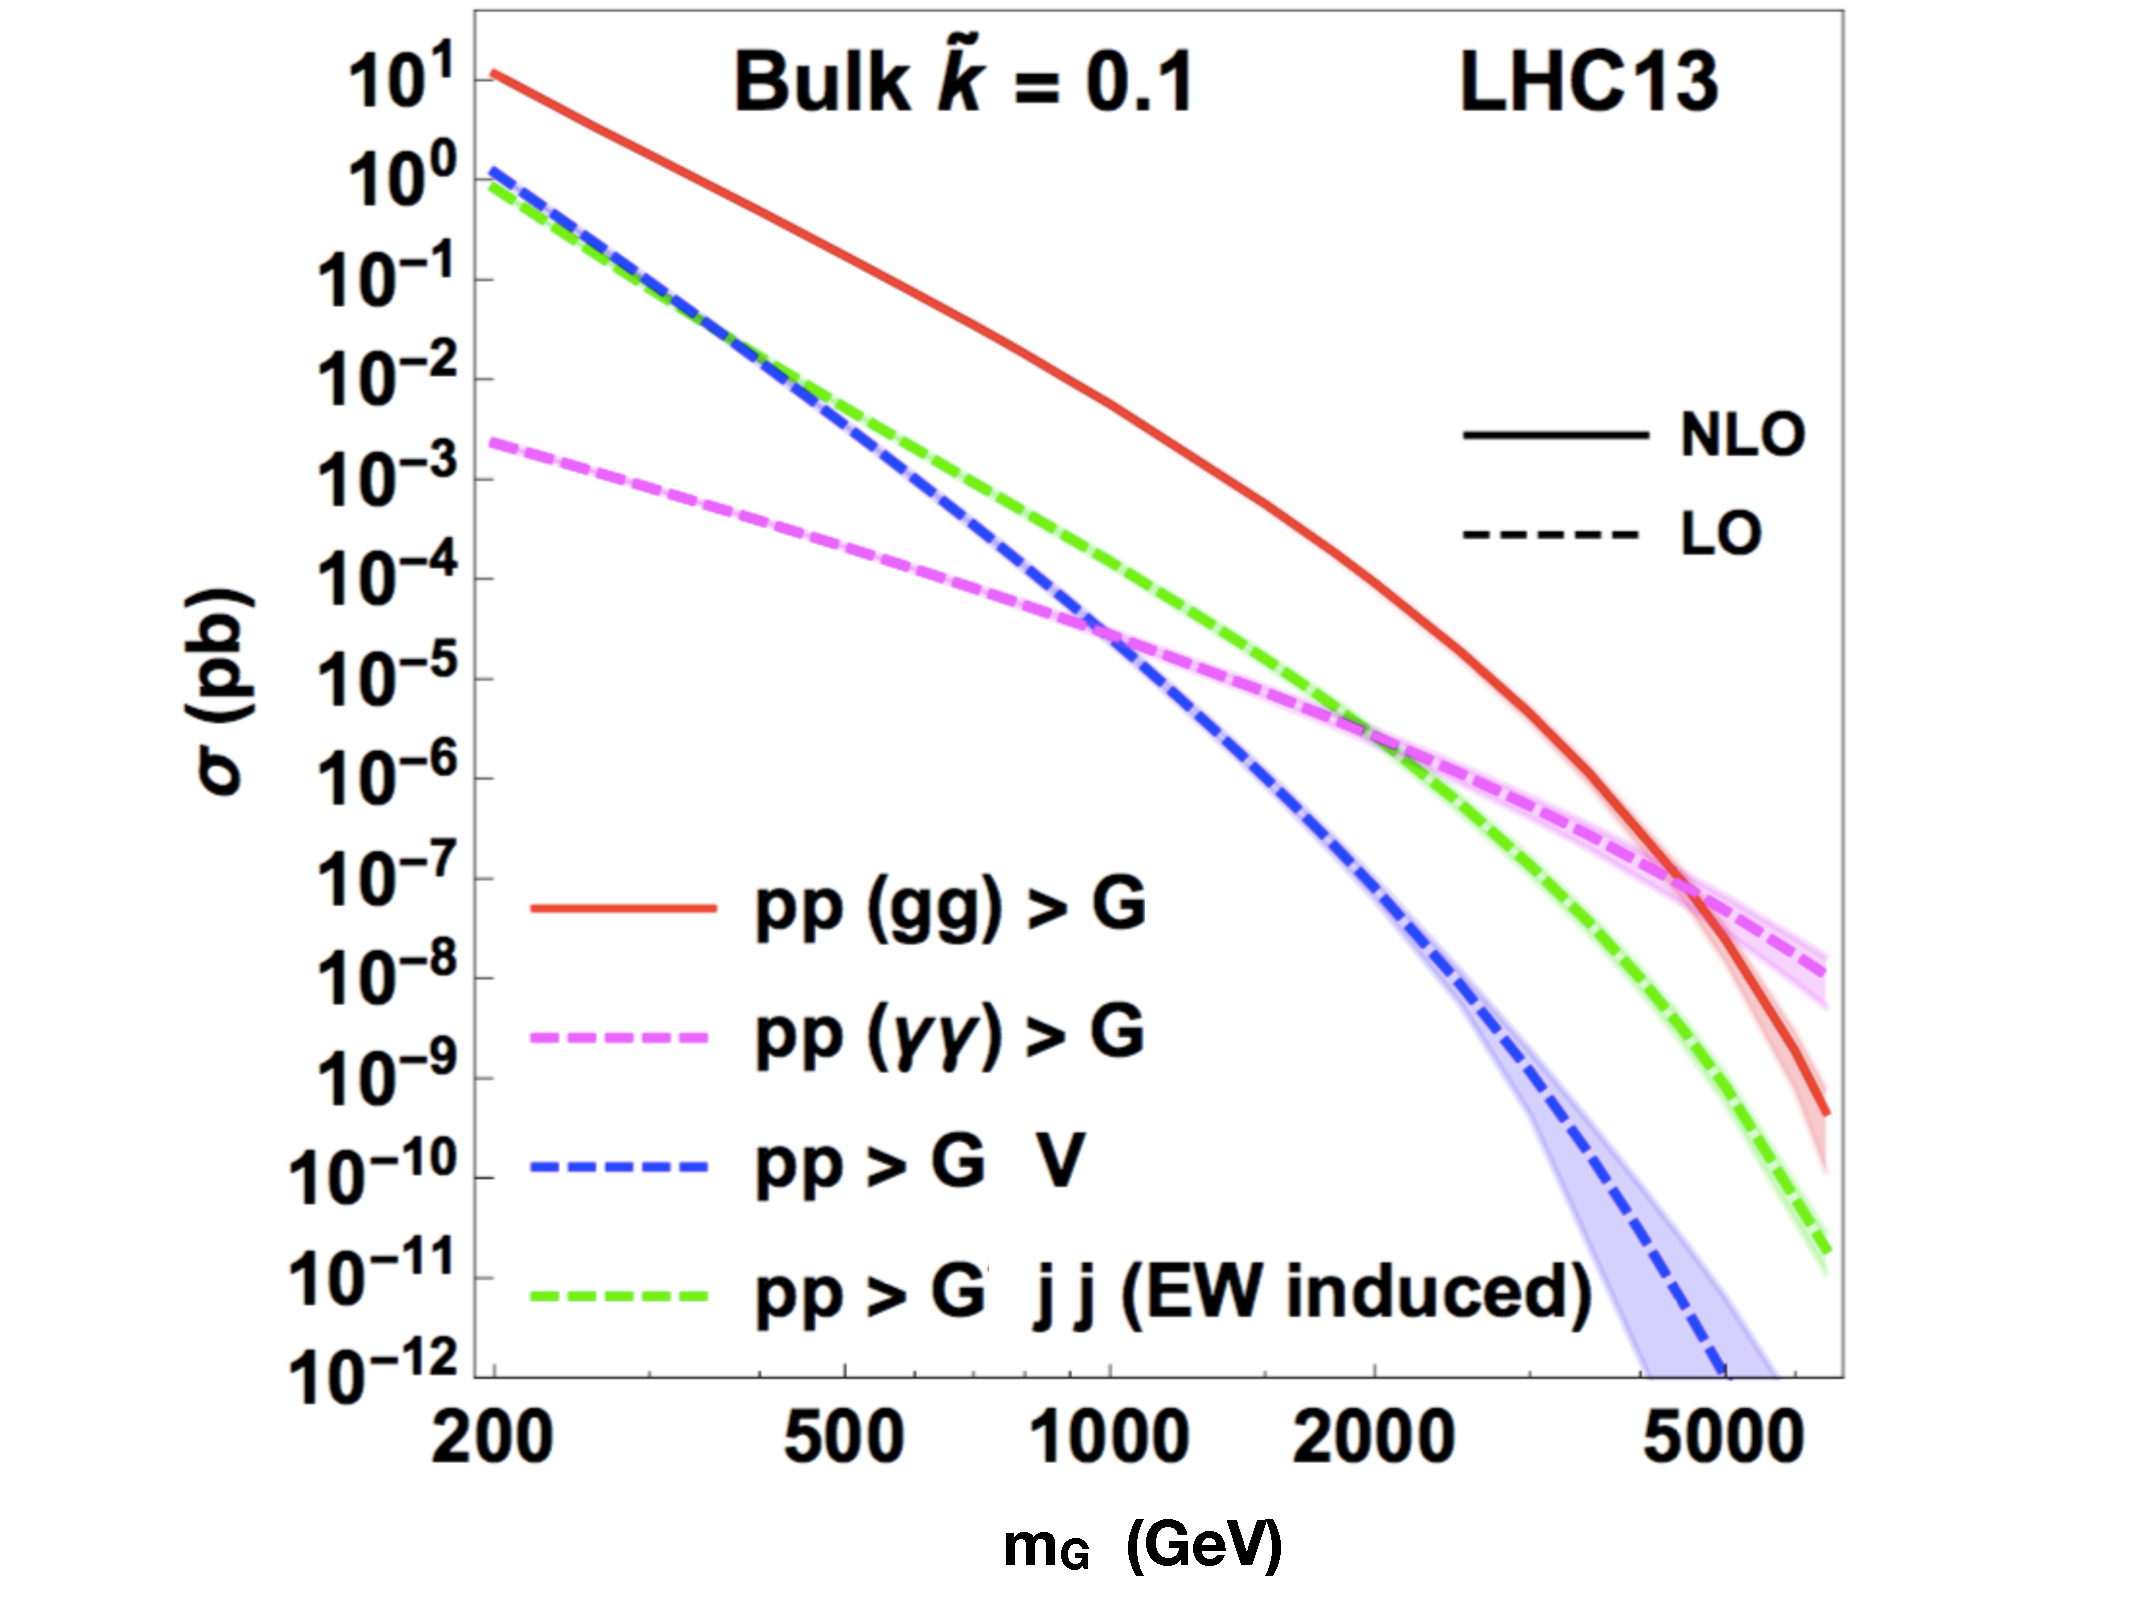
\includegraphics[width=0.5\linewidth]{figures/intro_Gxsec.pdf}
\caption{Production cross section for the K-K Graviton in the Bulk RS model, $\tilde{k}=0.1$}
\label{fig:intro_Gxsec}
\end{center}
\end{figure}
Here the $pp\rightarrow Gjj$ mode is dominated by the Vector Boson Fusion (VBF) process, and the $pp\rightarrow GV$ denotes the associated production with a massive vector boson. For $\tilde{k}<1$ and $m_{G}<2$ TeV the width of the K-K graviton is less than 6\% of the graviton mass, therefore a narrow resonance is expected. In this case the production cross section scales with $\tilde{k}$ as described in Equation~\ref{eqn:intro_kxsec}.
\begin{equation}
\sigma (m_G,\tilde{k}) = (\tilde{k}/0.1)^2 \sigma (m_G,\tilde{k}=0.1)
\label{eqn:intro_kxsec}
\end{equation}

In terms of the decay modes, the K-K gravitons are most likely to decay to SM particles localized near the TeV brane, as they have the strongest coupling to the graviton. Therefore the dominant decay modes are to top quarks and Higgs, as well as Z and W bosons, while the decay modes into massless gauge bosons and light quarks are suppressed and negligible. Figure~\ref{fig:intro_Gbr} shows the branching ratios for the decay of a Bulk Graviton.
\begin{figure}[htbp]
\begin{center}
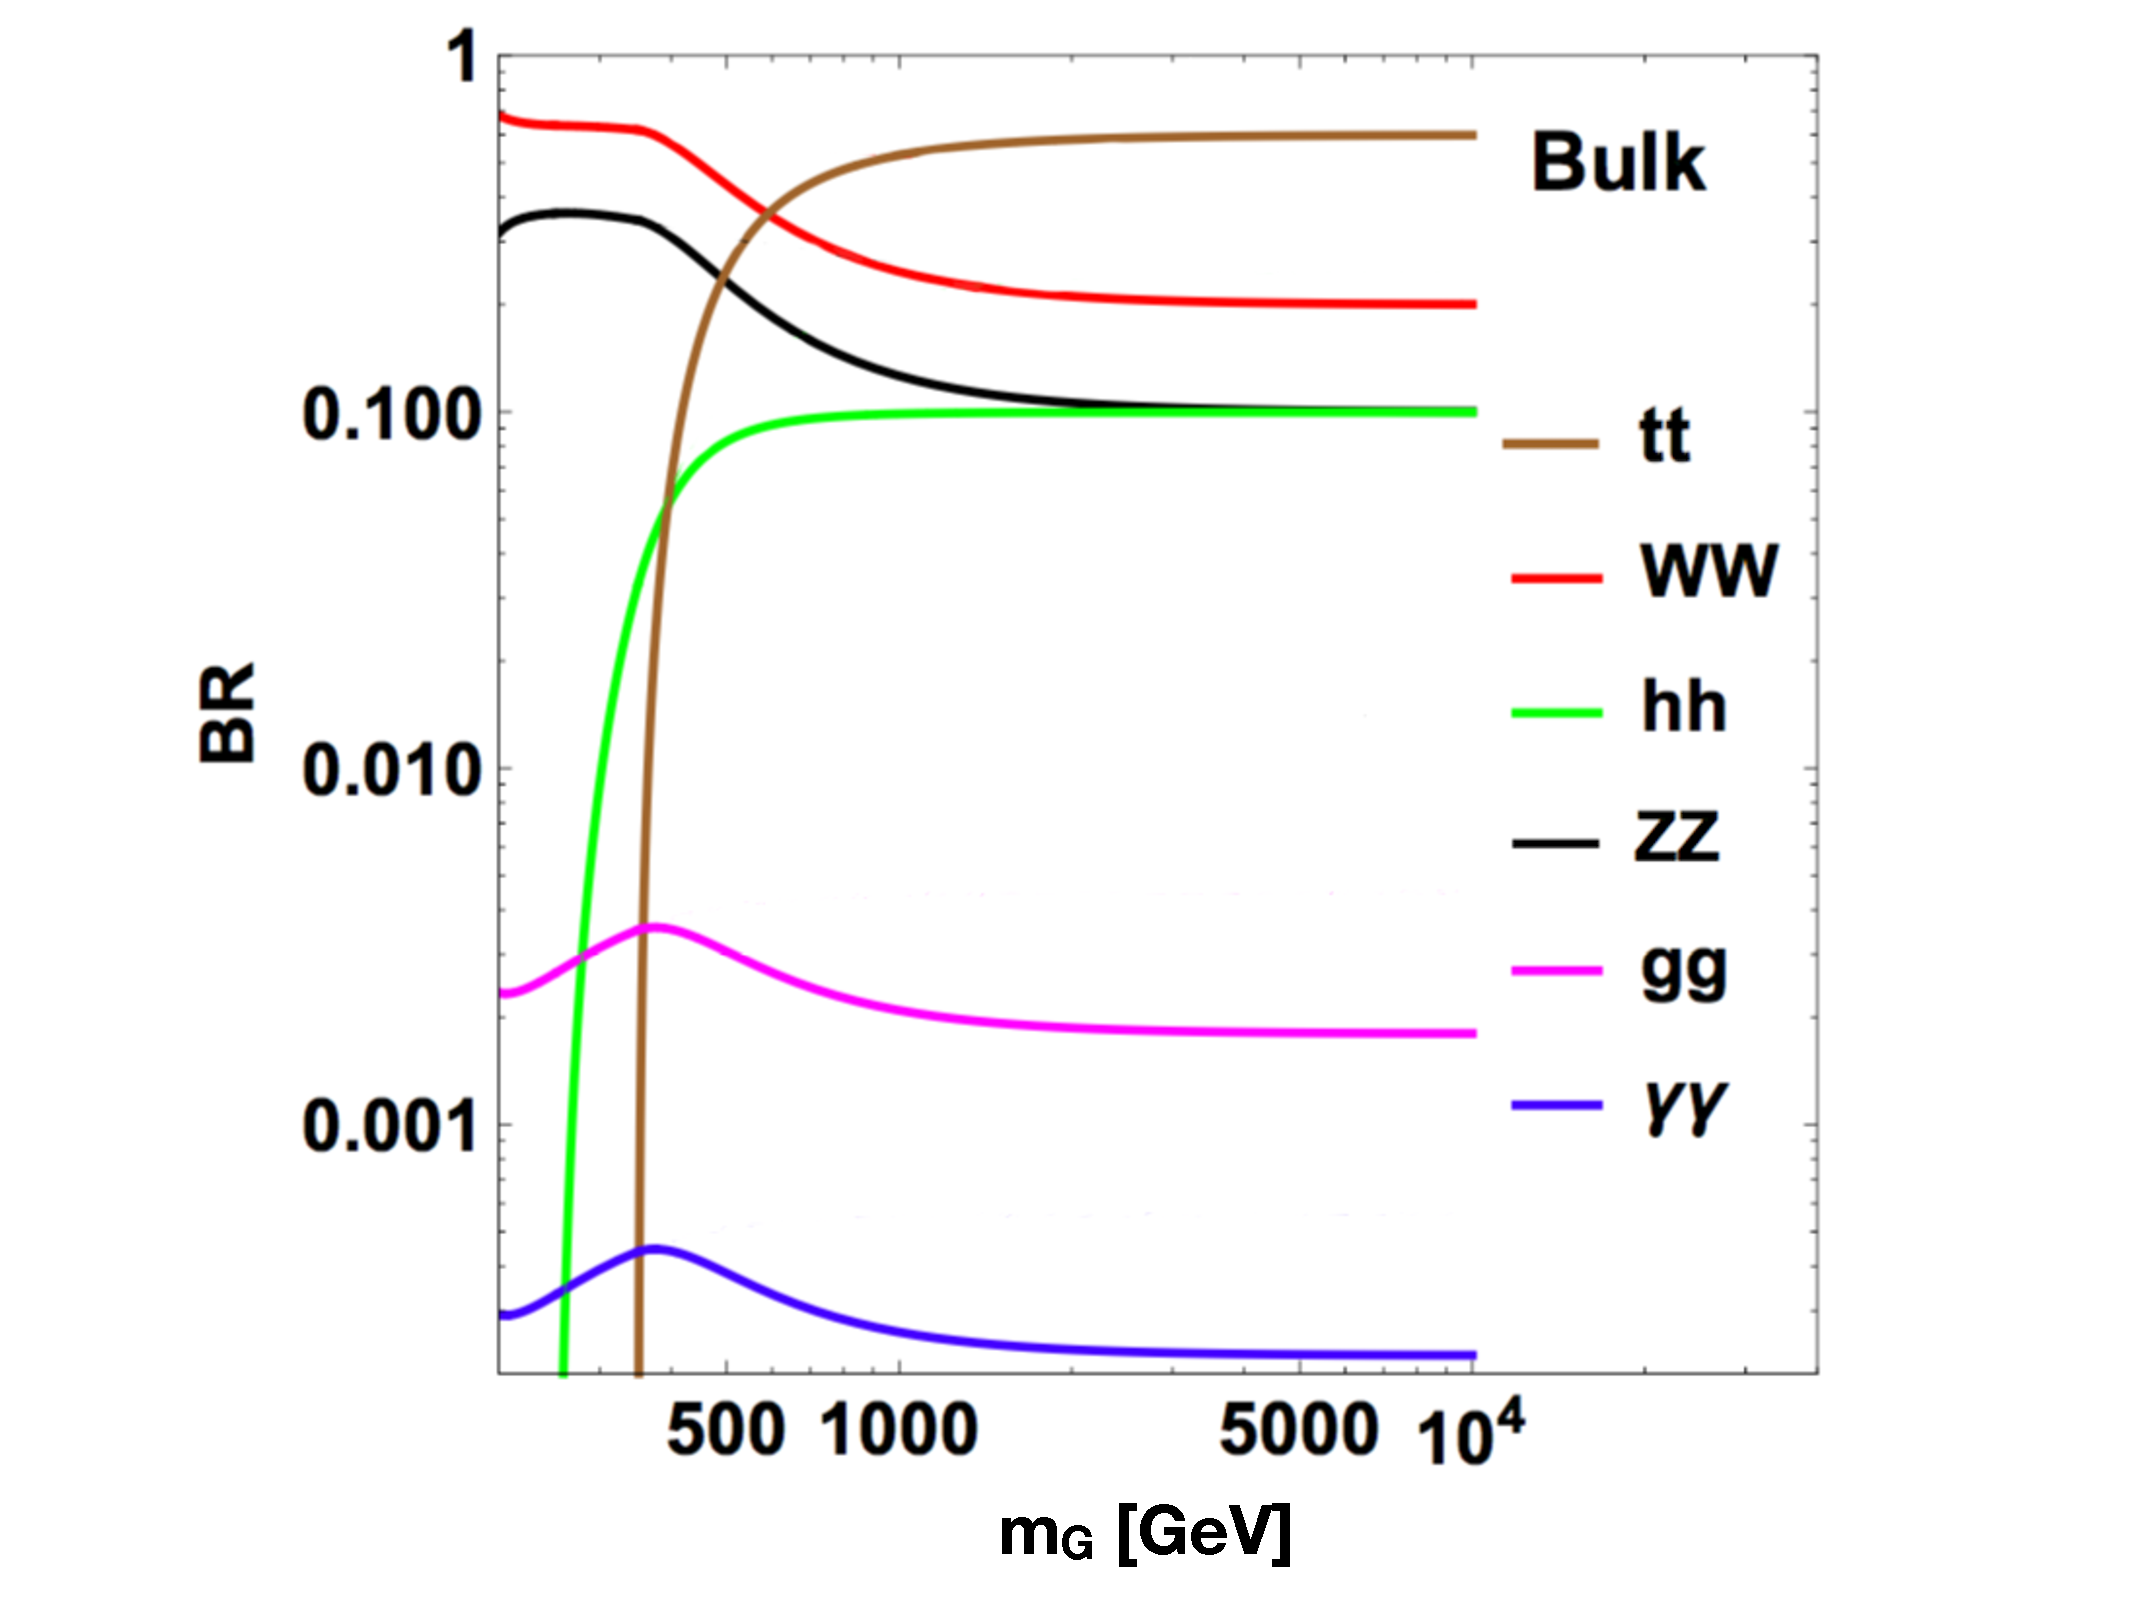
\includegraphics[width=0.5\linewidth]{figures/intro_Gbr.pdf}
\caption{Branch fraction of Bulk Graviton decay modes.}
\label{fig:intro_Gbr}
\end{center}
\end{figure}
The decay branching fractions are independent of $\tilde{k}$. Although the top channel and h channel have the highest branch fractions, neither of these channels can be easily detected or reconstructed. In contrast, despite of the relatively lower branching ratio, the W and Z boson channels are more preferred for the experimental search.

\section{Status of Searches for the Bulk Graviton} 
As described above, the Bulk Graviton can be produced by gluon fusion as well as other processes occurring in proton-proton collisions produced at the Large Hadron Collider. Because of the large gluon luminosity at the LHC, these data are ideally suited to search of evidence of a Bulk Graviton.
\subsection{Previous Searches}
Previous searches~\cite{Aad:2012nev,Aad:2013wxa,Aad:2014xka,Chatrchyan:2012baa,Khachatryan:2014gha,Aaboud:2016okv} for the Bulk Graviton have been performed based on data collected from both ATLAS and CMS detectors with the proton-proton center of mass energy at 7, 8 and 13\GeV. Limits on the cross section for the production of a Bulk Graviton have been set as a function of $m_{G}$. The existence of the Bulk Graviton was excluded with mass below 610\GeV~\cite{Chatrchyan:2012baa} for $\tilde{k}=0.5$ and mass below 1100\GeV~\cite{Aaboud:2016okv} for $\tilde{k}=1.0$ at 95\% confidence level. In these searches, semi-leptonic final states including leptons and jets, comprise the most popular channels. There is no previous search studying the channel ZZ to $2\ell 2\nu$.
\subsection{\boldmath{$2\ell 2\nu$} channel and  Search Strategy}
In this analysis we present a search for the Bulk Graviton or similar resonances decaying into a pair of Z bosons, in which one of the Z boson decays into a pair of charged leptons, either an electron pair or a muon pair (denoted by "$\ell$"), while the other decays into two neutrinos (denoted by "$\nu$"). Figure~\ref{fig:intro_llnndiagram} shows the Feynman diagram of this process. This analysis is based on the data from proton-proton collisions at a center-of-mass energy of 13 TeV collected by the CMS detector in 2016 and corresponding to an integrated luminosity of 35.9 fb$^{-1}$. 
\begin{figure}[htbp]
\begin{center}
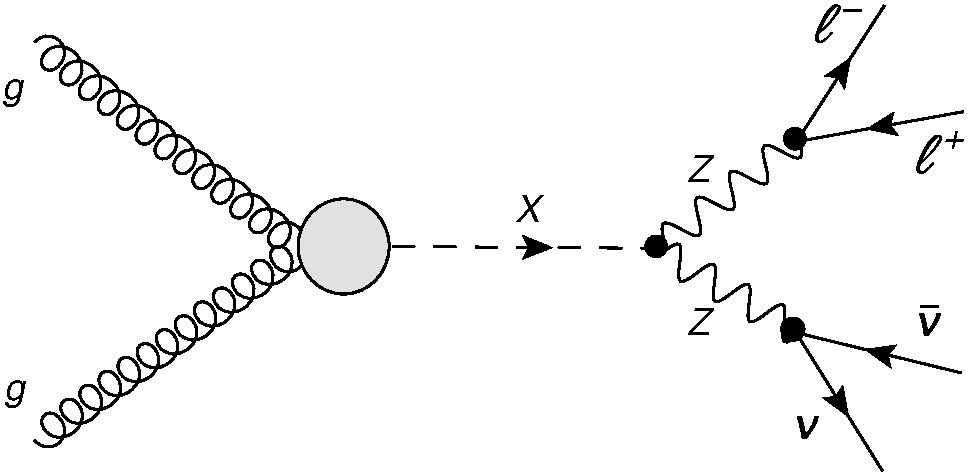
\includegraphics[width=0.72\linewidth]{figures/intro_llnndiagram.pdf}
\caption{Leading order Feynman diagram for the production of resonance X via gluon–gluon fusion decaying to the ZZ$\rightarrow 2\ell 2\nu$ final state}
\label{fig:intro_llnndiagram}
\end{center}
\end{figure}
The signature of the  $2\ell 2\nu$ channel is a pair of adjacent leptons with high transverse momentum ($p_T$) from the decay of a boosted Z boson and large missing transverse momentum from the other Z boson decaying to neutrinos, which is denoted as \ptmiss.

\vspace{0.3cm}
Compared to the semi-leptonic channels, the $2\ell 2\nu$ channel has reduced background. Although \Zjets production is a main source of background for both of these channels, it is almost impossible to distinguish the ZZ to $2\ell 2q$ process from \Zjets background, as they have very similar kinematics -- a Z boson and corresponding hadronic recoil. Unlike the \Zjets background, events from the ZZ to $2\ell 2\nu$ process always includes large \ptmiss, which makes it possible to strongly suppress the \Zjets background. Although the $2\ell 2q$ channel has a larger branching fraction, the branching fraction of the $2\ell 2\nu$ is still considerable, about 1/3 of that of the $2\ell 2q$ channel and 6 times as large as that for the four charged-lepton final state. The combination of lower statistics and the effects on resolution of a signal due to the undetected neutrinos explains why no previous search in $2\ell 2\nu$ channel was carried out. But now in RunII data with larger cross section from the higher collision energy and the larger and growing statistics, the $2\ell 2\nu$ channel has become more advantageous.

\vspace{0.3cm}
Because of the invisible neutrinos from the second Z boson decay, we will not have full momentum information for that Z boson, instead, only \ptmiss is available, which can be observed as the projection of the invisible Z boson's momentum on the x-y detector plane. Therefore it is not possible to reconstruct the invariant mass of the $2\ell 2\nu$ system. In this analysis the transverse mass ($m_{T}$) is designated as the discriminating variable to separate signal from background. The transverse mass variable is defined as:
\begin{equation}
m_{T}^2 = \left[ \sqrt{({p_{T}}^{\ell\ell})^2 + m^2_{\ell\ell}}
      + \sqrt{({p_{T}}^{miss})^2+m^2_{\ell\ell}}\right]^2
      - \left[\vec{p}_{T}^{\ell\ell}+\vec{p_{T}}^{miss}\right]^2,
\label{eqn:intro_MT}
\end{equation}

Here ${p_{T}}^{\ell\ell}$ and $m_{\ell\ell}$ each represent the $p_{T}$ and mass of the Z boson constructed from the charged lepton pair system. The $m_{\ell\ell}$ in the middle term provides an estimator of the mass of the invisibly decaying Z boson. This choice has negligible impact on the expected signal at large $m_{T}$, but is found to preferentially suppress backgrounds from $t\bar{t}$ and WW decays.

\vspace{0.3cm}
Although the $m_{T}$ variable only equals the invariant mass confined to the transverse plane, a kinematic edge is still expected from the putative heavy resonance, and the position of the edge strongly depends on the mass of the resonance. Figure~\ref{fig:intro_mt} gives an example of what the transverse mass spectrums look like from the decay of resonances with invariant masses each at 800\GeV, 1000\GeV, 1200\GeV and 1400\GeV. The kinematic edges on the right side of each spectrum are very close to the graviton mass values.

\begin{figure}[htbp]
\begin{center}
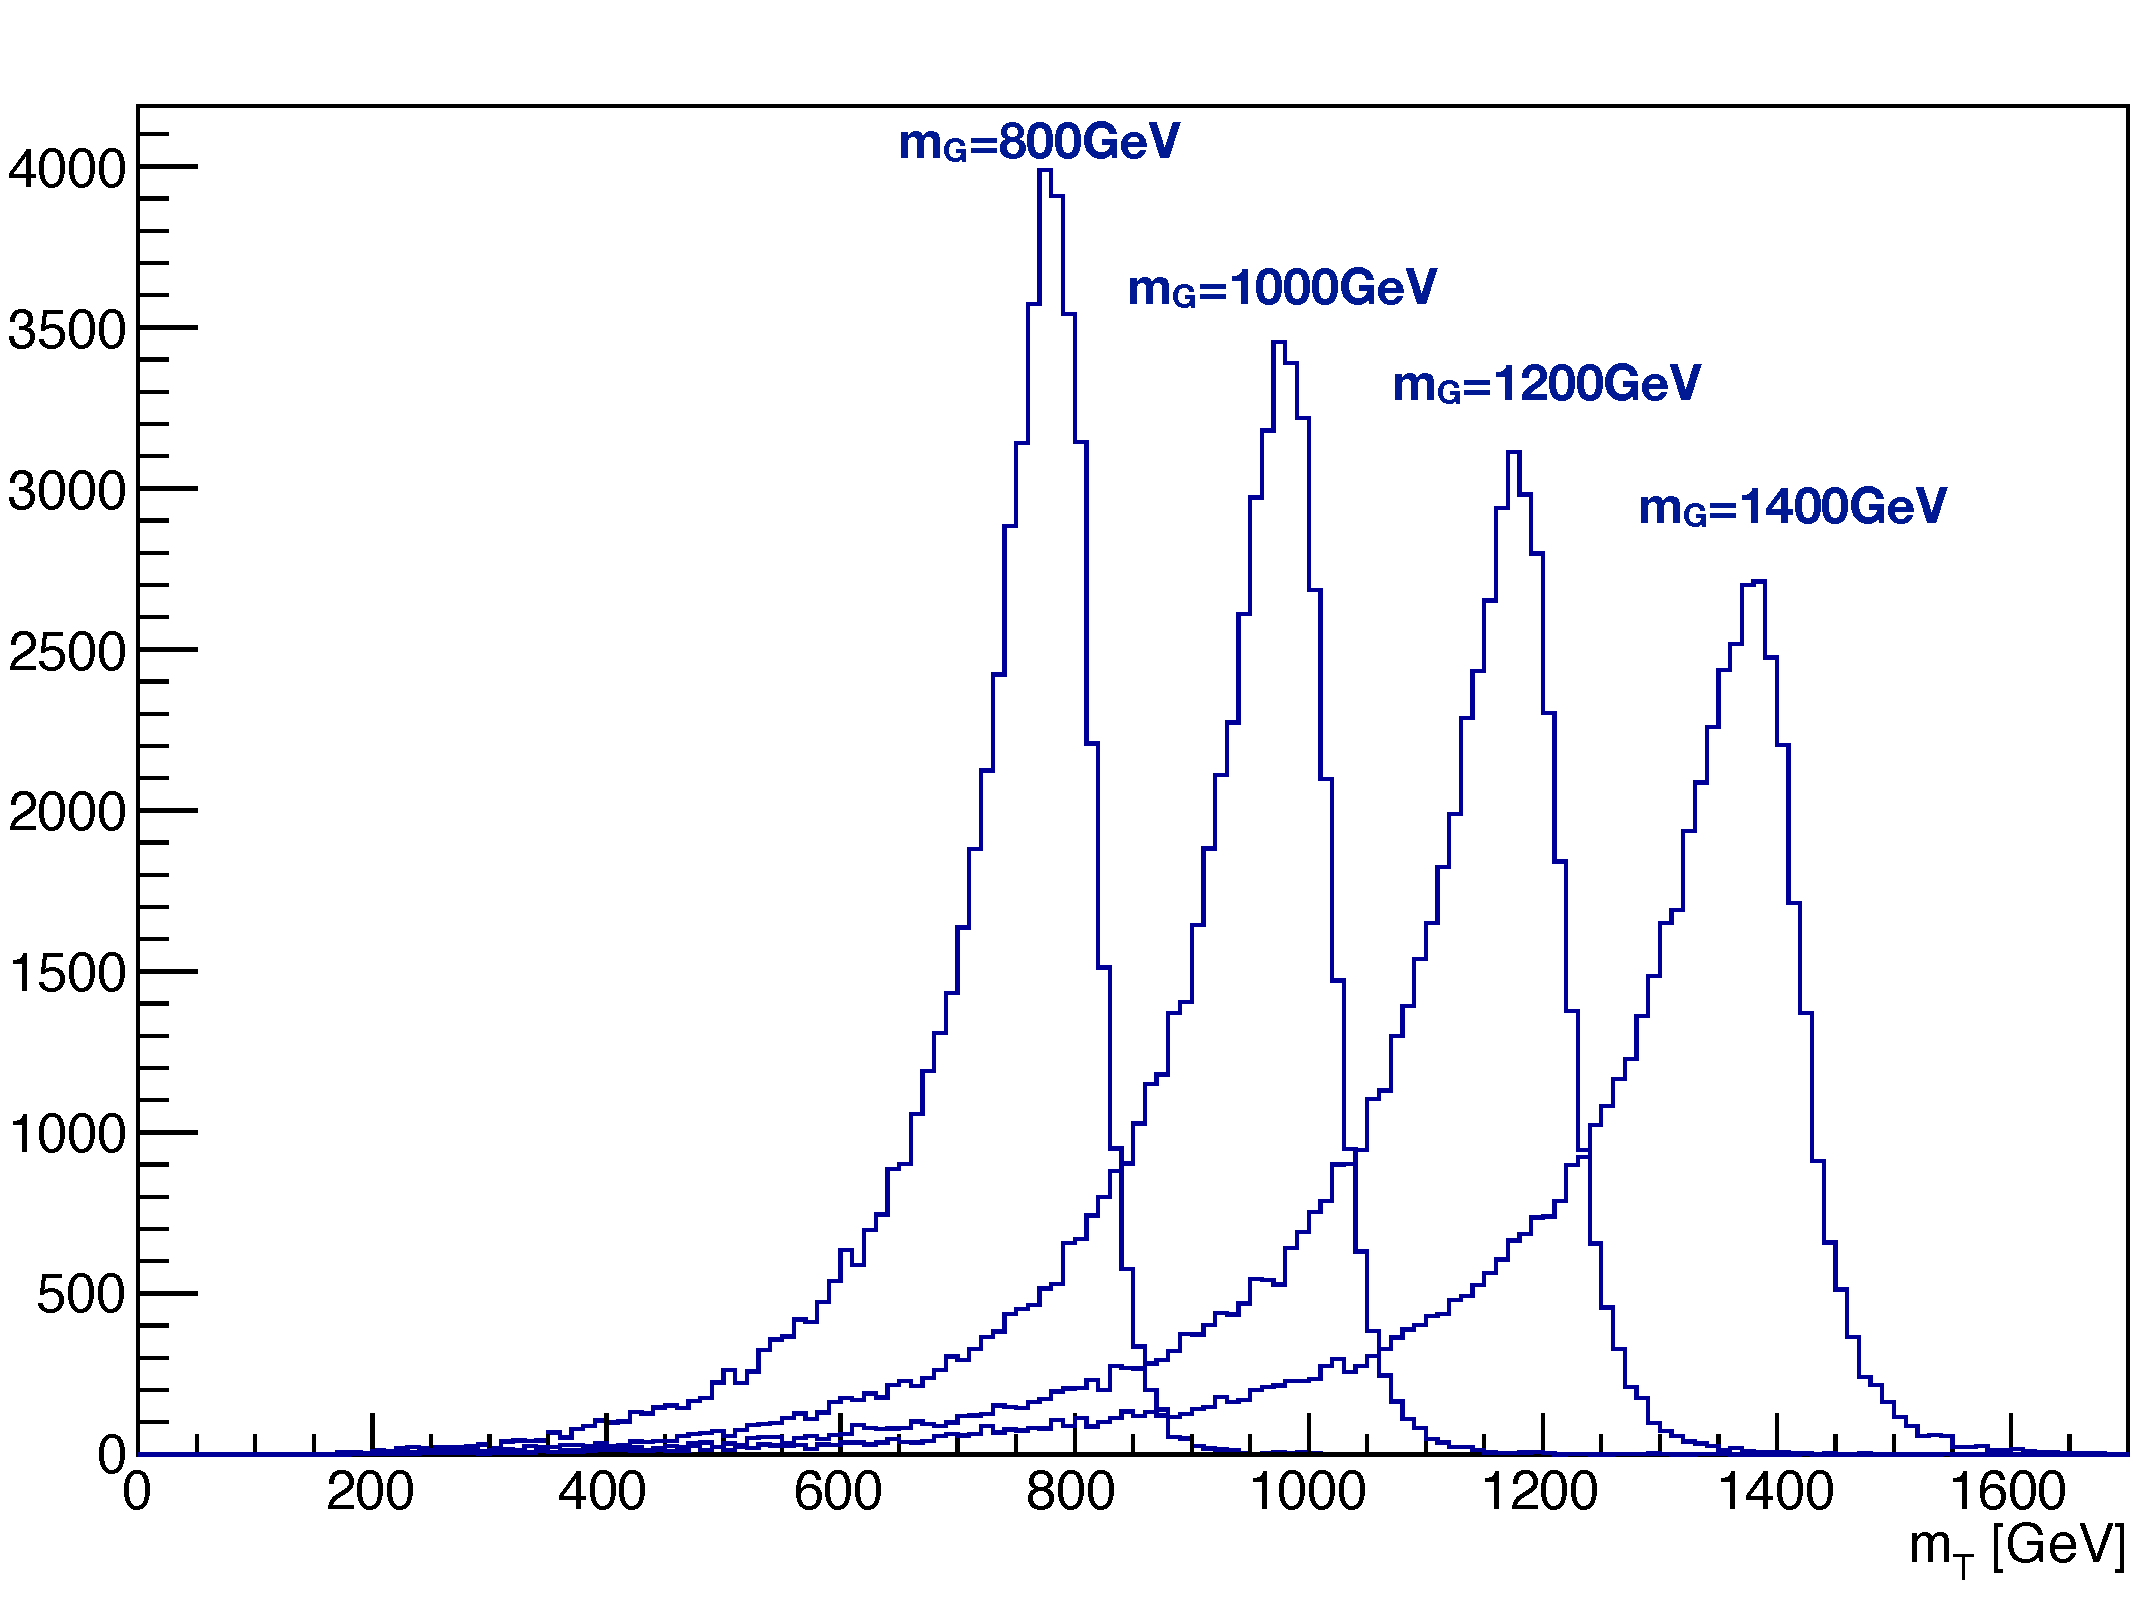
\includegraphics[width=0.72\linewidth]{figures/intro_example_mt.pdf}
\caption{The transverse mass($m_{T}$) spectrums of resonances with masses at 800\GeV, 1000\GeV, 1200\GeV and 1400\GeV.}
\label{fig:intro_mt}
\end{center}
\end{figure}

\vspace{0.3cm}
The transverse mass can also be written in an alternate form in which no vector is involved:
\begin{small}
\begin{equation}
m_{T}^2 = \left[ \sqrt{({p_{T}}^{\ell\ell})^2 + m^2_{\ell\ell}}
      + \sqrt{({p_{T}}^{miss}_\perp)^2+({p_{T}}^{miss}_\parallel)^2+m^2_{\ell\ell}}\right]^2
      - \left({p}_{T}^{\ell\ell}+{p_{T}}^{miss}_\parallel\right)^2
      - ({p_{T}}^{miss}_\perp)^2,
\label{eqn:intro_MTalt}
\end{equation}
\end{small}
where ${p_{T}}^{miss}_\parallel$ refers to the projection of \ptmiss in the direction of ${p}_{T}^{\ell\ell}$ and ${p_{T}}^{miss}_\perp$ is the fraction perpendicular to ${p}_{T}^{\ell\ell}$.

%\section{CMS and Me} %what did i do in this analysis and others
%In August 2014, I joined the UVA CMS group and worked on calibrating a prototype Shashlik calorimeter using the muon data as my first project here. Aferwards, in the middle of 2015, I left for CERN, Switzerland and stayed there for 2 years. During my stay at CERN I was involved in several projects and activities both on the detector and physics analysis. 

%\vspace{0.3cm}
%My most detector-related work focused on the Hadron Calorimeter(HCAL). Starting with the Hadron Forward (HF) detector frontend electronics Phase I upgrade in 2015. I joined the HCAL upgrade team, helping design and carry out a series of electronics tests. In 2016 I helped the HCAL Endcap (HE) upgrade with the system monitoring, and HCAL Data Quality Management (DQM) group with their online DQM system for the HF/HE upgrades. I was also taking the HCAL detector on call expert shifts continually for 1 year and a half since 2016.

%\vspace{0.3cm}
%In terms of physics analysis, I started working on this di-boson analysis in the December of 2015, helping to design and implement the analysis framework from scratch, studying the pileup reweighting, trigger efficiency, lepton identification algorithms and their efficiencies, as well as determining the non-resonant background using data-driven modeling. The muon tracker High $p_{T}$ efficiency calculated by me has been widely used in related CMS analyses and I am also contributing to the high $p_{T}$ muon paper carried out by the muon Physics Object Group (POG). Apart from this di-boson analysis, I also worked as the generator contact person for physics simulations in the Beyond Two Generations (B2G) Physics Analysis Group (PAG) for the whole year of 2017.

\chapter{The LHC and CMS detector}
This analysis is based on the 2016 data collected in the CMS experiment. The Compact Muon Solenoid (CMS) experiment is a detector built on the Large Hadron Collider (LHC) located at CERN, Switzerland. This chapter gives an overview of LHC and CMS experiment.

\section{The Large Hadron Collider} 
The Large Hadron Collider (LHC) is the world most powerful particle accelerator and collider. It was built by the European Organization for Nuclear Research (CERN) between 1998 and 2008, in the tunnel of its predecessor, the Large Electron Positron Collider (LEP), with a circumfence of 27 km and as deep as 175 metres (574 ft) beneath the France–Switzerland border near Meyrin, Geneva. 
\vspace{0.3cm}
The process of particle acceleration begins from a simple tank of hydrogen as the source of protons, which are progressively accelerated to higher energies in sequential machines ending at the LHC. A diagram of the CERN accelerator complex is shown in Figure~\ref{fig:lhc_lhc}. Over 1000 dipole magnets are used to produce a magnetic field of 8.3T and bend the proton beams onto the circular trajectory. 
\begin{figure}[htbp]
\begin{center}
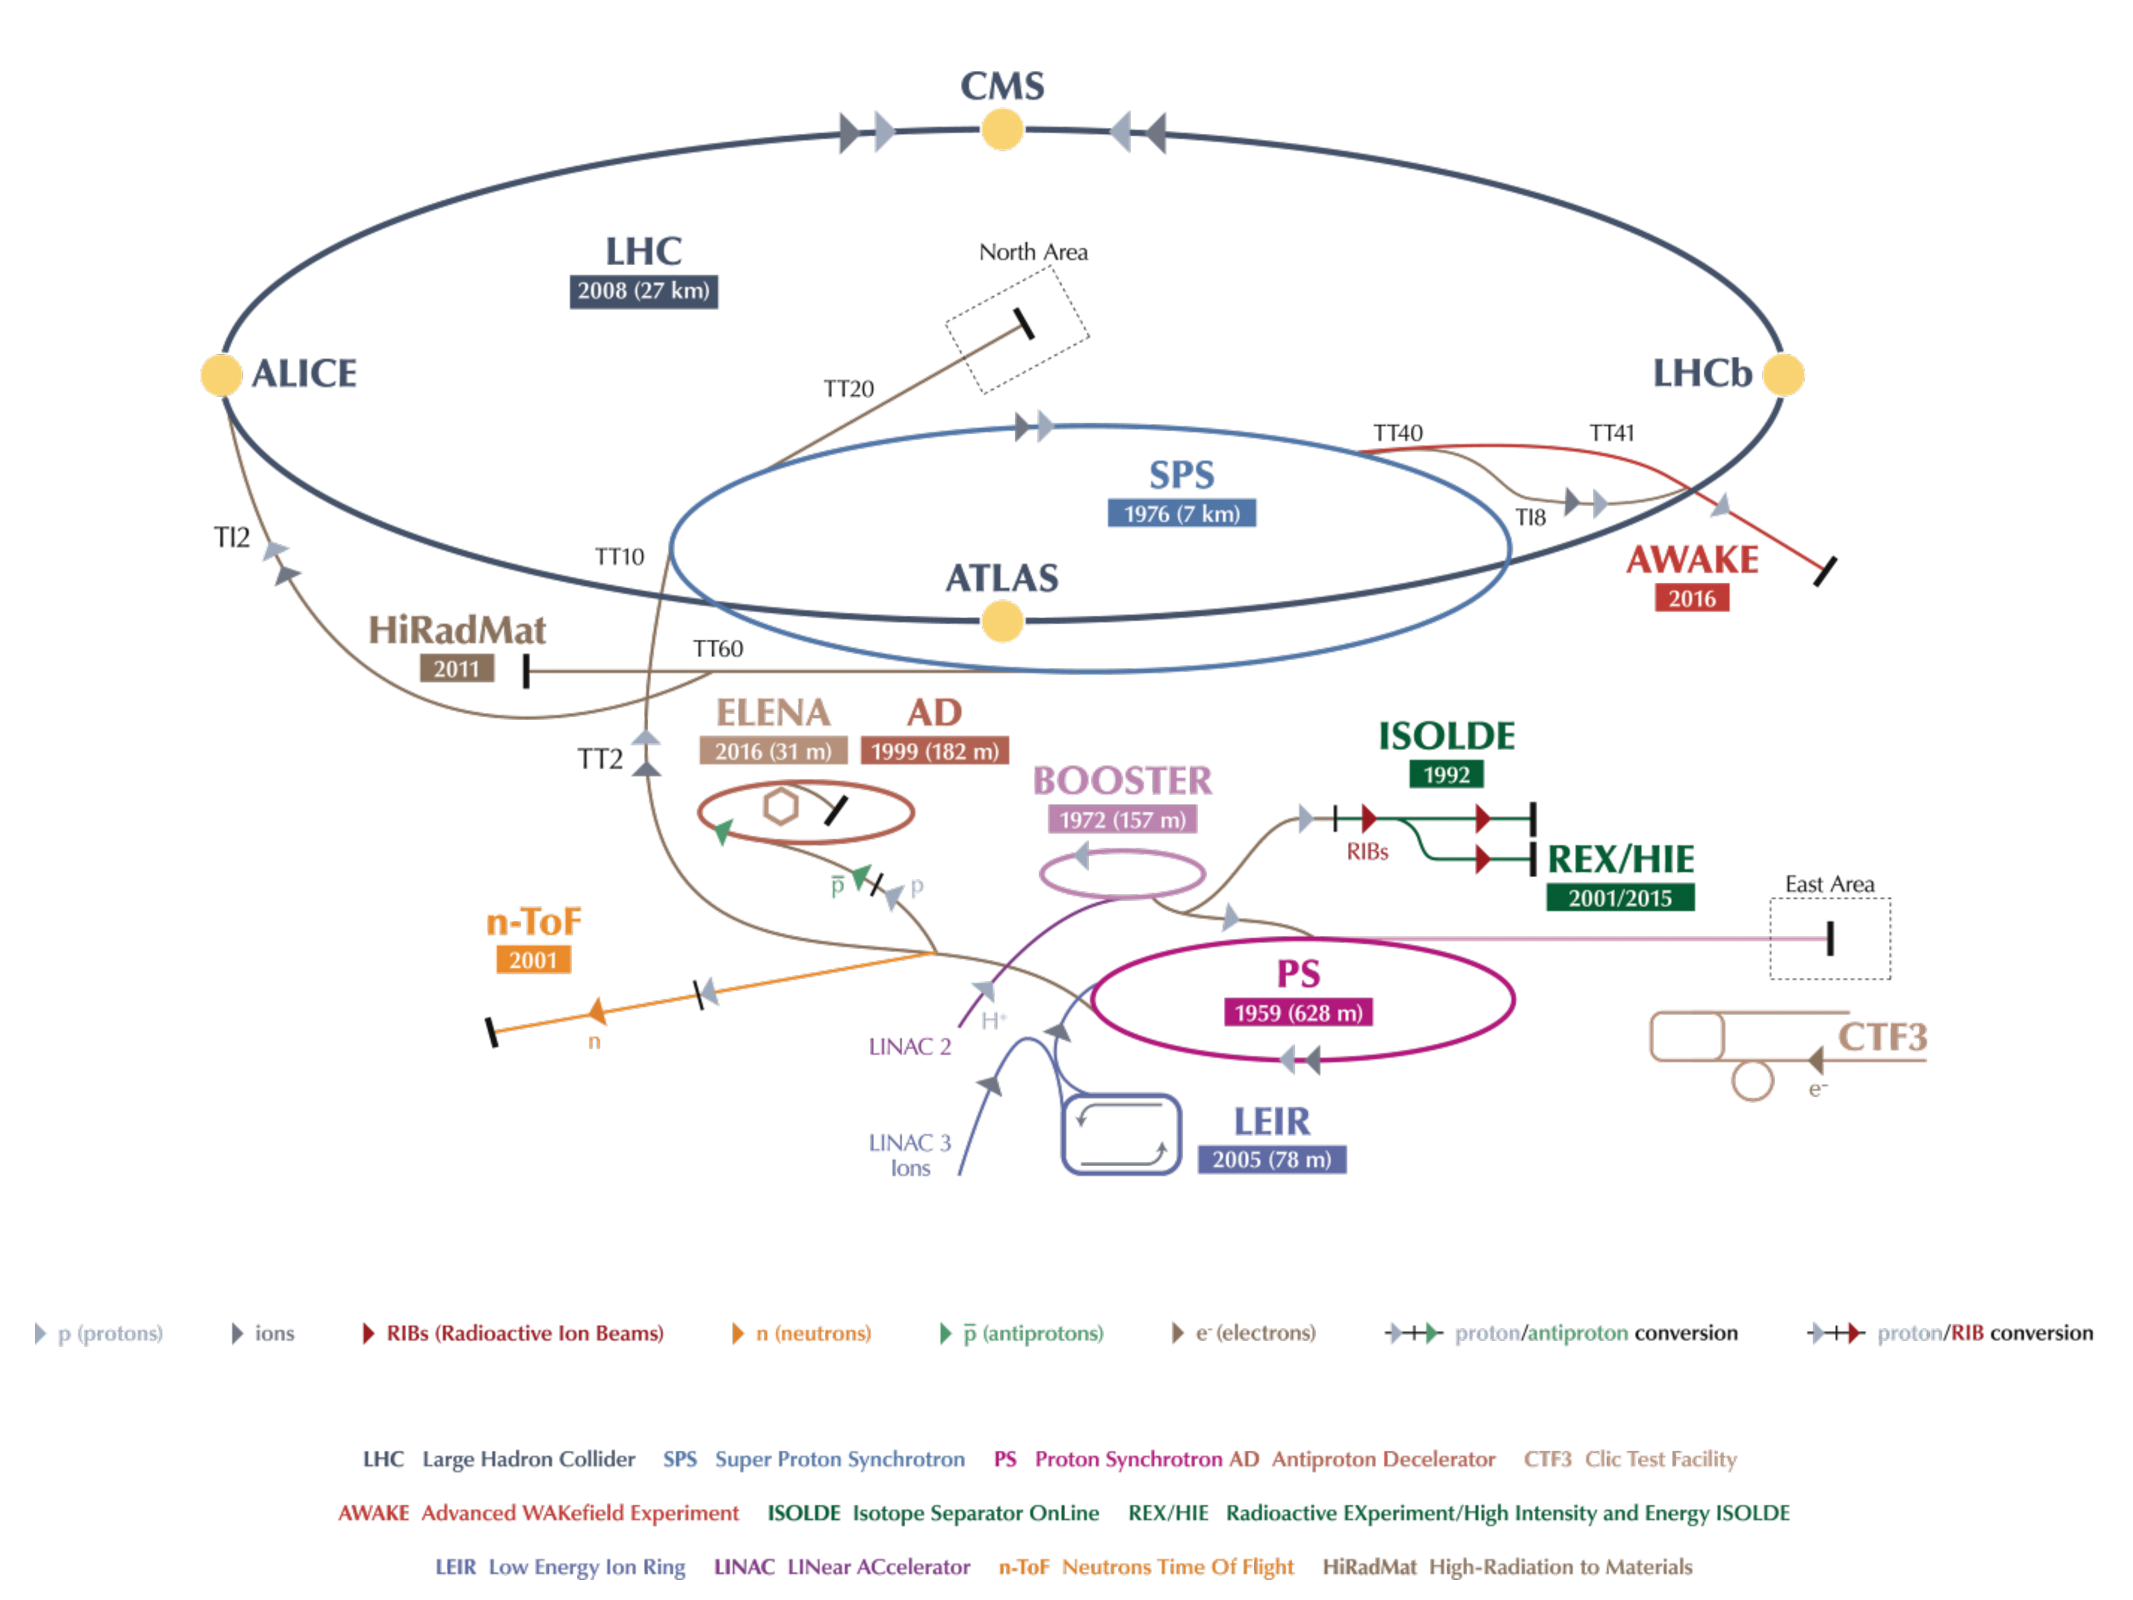
\includegraphics[width=0.72\linewidth]{figures/lhc_lhc.pdf}
\caption{CERN accelerator complex including the four main experiments and the injection chain}
\label{fig:lhc_lhc}
\end{center}
\end{figure}

\vspace{0.3cm}
Inside LHC particle collisions can happen at 4 interaction points of the tunnel, which correspond to 4 experiments: CMS, ALICE, ATLAS and LHCb. The ALICE experiment is designed to study the quark-gluon plasma using data collected during the heavy ion operation on the LHC. These measurements are designed to draw conclusions about the initial state of the universe. LHCb focuses on precisely measuring B-meson decays and CP-violating processes. CMS and ATLAS are the two general purpose experiments at the LHC build for studying a broad range of physics processes. These studies include precision measurements of Standard Model processes and parameters, thereby deepening our knowledge and understanding of the Standard Model. In addition, major fields of study are searches for the Higgs bosons and study of their properties and searches for physics beyond the Standard Model.

\section{The Compact Muon Solenoid (CMS) Experiment}

\subsection{Tracker} 
\subsection{Calorimeters} 
\subsubsection{Electromagnetic Calorimeter} 
\subsubsection{Hadronic Calorimeter} 
\subsection{Muon Chambers} 
\subsection{Data Acquisition and Trigger System} 

\chapter{Physics Objects Reconstruction}
The information recieved from the detector is in the format of detector hits and electrical signals, which is not directly suitable for physics analyses. In this chapter we introduce the reconstruction and identification of physics particles involved in this analysis, based on the detector-level information. 

\vspace{0.3cm}
The Particle-Flow algorithm~\cite{ob_pf} is used for event and particle reconstructions.

\section{Particle Flow Algorithm}
The PF algorithm starts from reconstructing the basic PF elements including the trajectories of charged particles, electron/muon tracks and calorimeter clusters, based on the information collected from each subsystem of the detector. Then a link algorithm is used to form a block of these PF elements possibly related to a single physics object. Afterwards, the particle constructions and identifications are processed based on the blocks. The constructions of the PF elements are described briefly as below.

\subsection{Charged-particle tracks and vertices}
The construction of charged-particle tracks provides supports for particle reconstructions and identifications, including the measurement of the momentum of energetic and isolated muons, identification of energetic and isolated hadronic $\tau$ decays, and tagging b quark jets. A combinatorial track finder based on Kalman Filtering (KF) is used for track construction~\cite{ob_trackconst1,ob_trackconst2}. It starts with a few hits compatible with a charged-particle trajectory in the tracking system; and then finds hits from all the tracker layers along this charged-particle trajectory; and finally performs fitting to determine the trajectory and the particle properties including origin, transverse momentum and direction. To increase the reconstruction efficiency and suppress the fake rate, the combinatorial track finder was applied in several successive iterations.

\vspace{0.3cm}
The vertex reconstruction aims at determine the locations of all the proton-proton interactions and uncertainties in each event. The vertex reconstruction uses the information of the reconstructed charged-particle tracks. After determining the candidate vertices with the deterministic annealing (DA) algorithm and fitting them with at least two matched tracks using an adaptive vertex fitter, good vertices are selected with quality criteria including being consistent with the collision region (referred to as beam spots) and matched to a minimum of four tracks. The primary vertex of an event is considered to be the vertex with the largest sum of the squared track momenta. And the other vertices are regarded as pile-up vertices. Figure~\ref{fig:ob_Nvertex} shows the vertices number distribution for the data collected in 2016.
\begin{figure}[htbp]
\begin{center}
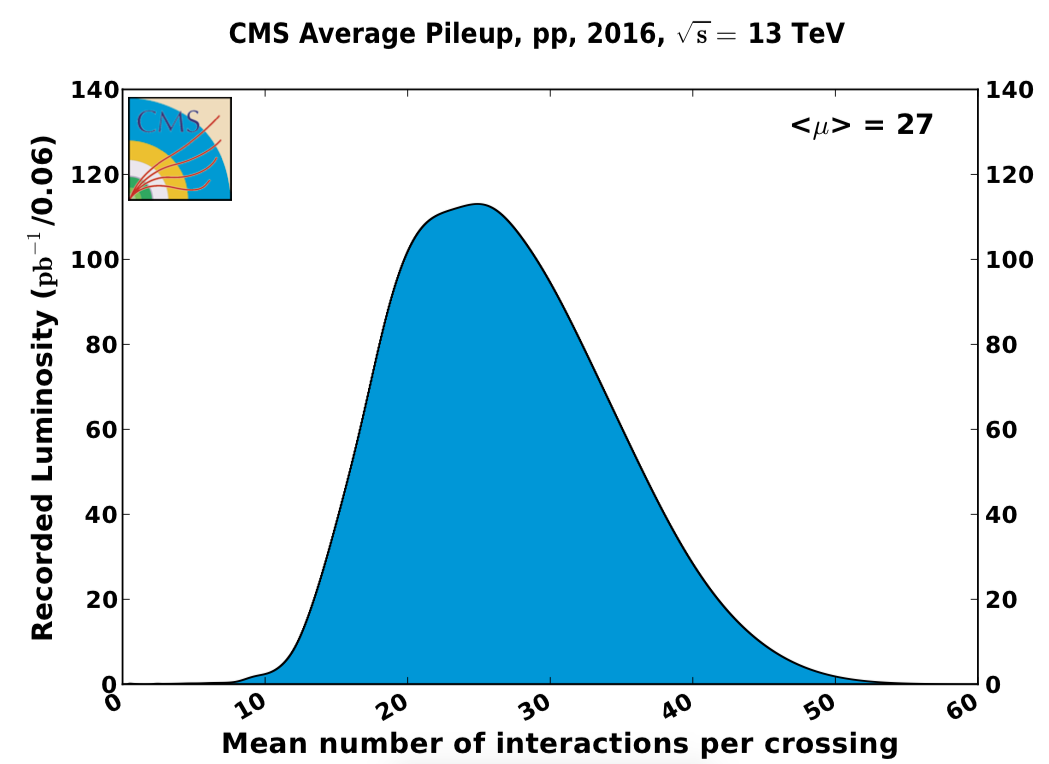
\includegraphics[width=0.72\linewidth]{figures/ob_Nvertex.png}
\caption{Number of interactions per bunch crossing for data collected in 2016.}
\label{fig:ob_Nvertex}
\end{center}
\end{figure}

\subsection{Calorimeter clusters}
The calorimeter clustering serves four purpose in general: detect and measure the energy and direction of stable neutral particles; separate these neutral particles from charged hadron energy deposits; reconstruct and identify electrons and all accompanying bremsstrahlung photons; and help the energy measurement of charged hadrons for which the track parameters were not determined accurately. An algorithm is developed and the clustering process is performed seperately for EB, EE, ES, HB and HE. Firstly cluster seeds are selected as calorimeter cells with deposited energy larger than a threshold and its neighbouring cells. The topological clusters then spread from the seed to the nearby cells with energy beyond cerntain thresholds. Finally a fitting for each topological cluster is performed based on an expectation-maximization algorithm to evaluate position and amplitude of the particle clusters. 

\subsection{Tracks for electrons}
Because of the significant tracker thickness, most of the electrons emit considerable fraction of their energy in the form of bremsstrahlung photons before reaching the ECAL. To reconstruct the properties of an electron, the energy of the bremsstrahlung photons in ECAL must be taken into account as well, apart from the energy deposited by the final electron. A tracker-based electron seeding method was developed. When the radiated energy is small, the electron track can be reconstructed across the whole tracking system with a well-behaved fit $\chi^2$, and the reconstructed momentum should match the energy deposited in the corresponding ECAL cluster. However when energetic photons are radiated, the momentum change of the electron will lead to a large $\chi^2$ and missing hits in the tracker. In these cases, a selection of tracker hits are performed based on the $\chi^2$ value and number of hits in the previous KF fit, and these selected hits are fit again with a Gaussian-sum filter (GSF)~\cite{ob_electronconst} which is more adapted to the electrons as energy losses along the trajectory are considered. 

\subsection{Tracks for muons}
The muons leave their trajectories in the tracking system where the momenta of the muons can be precisely measured, and can be well identified over the full detector especially with the muon chambers. Hits within the DT and CSC detector are clustered to form track segments. These track segments are then used as seeds to reconstruct the muon trajectory throughout DT, CSC, and RPC hits. The result of the final fitting is refered to as a standalone-muon track. With the information of the reconstructed tracks in the tracking system, two collections of high-level muons physics objects can be obtained: the global muon and the tracker muon (See Section~\ref{sec:muonrecon}).

\subsection{Link algorithm}
To reconstruct a physics object, a link algorithm is applied to connect the related PF elements from different subdetectors. The PF elements that can be considered by the algorithem can only be the nearest neighbours in the ($\phi$,$\eta$) plane to any of the elements in the linked block starting from a seed element. The element will be added to the block after the distance of the link is examinated. This process continues until the PF block is formed and the reconstruction of the corresponding particle starts. Links between GSF electron tracks and the ECAL clusters can be established for electrons; links among calorimeter clusters can be established for various particle reconstruction processes, specifically trivial links among ECAL clusters with close $\eta$ but spread $\phi$ form link blocks called superclusters; links between tracks and muon segments can be established for muon reconstruction.

\section{Electron Reconstruction}
The electron reconstruction and identification are performed mainly based on the information from electron tracks in the tracking system and the ECAL clusters. ~\cite{ob_electronconst2}

\vspace{0.3cm}
The electron reconstruction starts from a GSF electron track. In the link algorithm, apart from the electron cluster in ECAL, clusters nearby the extrapolated tangents of the GSF track will also be linked to the PF block as potential bremsstrahlung photons emitted from the electron. A GSF track will be considered a electron candidate if in the PF block the ECAL cluster corresponding to the electron shower is not linked to more than 2 tracks. 

\vspace{0.3cm}
The ECAL clusters in the PF block that can be linked to either the GSF track tangents or the supercluster will be associated with the candidate electron and will be used for the energy calculation of the electron. So is the GSF track if the momentum calculated agrees with the energy deposited in the calorimeters. The position information ($\eta$,$\phi$) assigned to the electron is obtained from the GSF tracks. Once an element is assigned associated to a reconstructed particle, it will be masked against further processing in other object constructions. The calculated energy from the calorimeter clusters will be corrected in terms of energy and $\eta$, to compensate the energy loss in the process. And the final energy assigned to the electron will be obtained from a combination of the corrected energy from the calorimeter clusters and the momentum of the GSF track. 

\vspace{0.3cm}
Furthermore, electrons used in physics analyses must meet additional identification and isolation requirements.

\subsection{Electron Identification and Isolation}
The electron candidates used in this analysis are required to pass the \texttt{loose} cut-based identification (ID) and isolation (Iso) recommended by the CMS EGamma Physics Object Group (POG) for 2016 data.

The ID and Iso criteria set cuts on the following variables, and the cut values are given in Table~\ref{tab:electron-id}.

\begin{itemize}%[noitemsep,nolistsep]
\item the $\eta_{\rm SC}$ denotes the $\eta$ value of the corresponding ECAL super cluster;
\item the $\sigma_{i\eta,i\eta}$ describing the shape of the supercluster;
\item the geometric distance, $|\Delta\eta_{in}|$ and $|\Delta\phi_{in}|$, between the supercluster and the matched track;
\item the ratio of the energy deposits in HCal and ECAL, \texttt{hOverE};
\item the relative combined PF isolation following correction for
  pile-up contamination in the
  Effective Area (EA), \texttt{relIsoWithEA}; % it is the pf Iso used in our analysis 
\item the difference between the tracker momentum and ECAL energy, $|1/E-1/p|$;
\item the maximal expected missing inner hits;
\item a veto on the electrons that are likely to be produced by photon conversions.
\end{itemize}



\begin{table}[htb!]
  \center
  \caption{The cuts used in the POG \texttt{loose} electron identification.}
  \label{tab:electron-id}
  \begin{tabular}{r c c c}
    \hline
    Variable & Barrel & Endcap \\
    \hline
    $|\eta_{\rm SC}|$ acceptance & $(0, 1.479)$ & $(1.479, 2.5)$\\
    $\sigma_{i\eta,i\eta} <$ & 0.011  & 0.0314 \\
    $|\Delta\eta_{in}| <$ & 0.00477  & 0.00868 \\
    $\Delta\phi_{in} <$ & 0.222  & 0.213 \\
    \texttt{hOverE} $<$ & 0.298  & 0.101 \\
    \texttt{relIsoWithEA} $<$ & 0.0994  & 0.107 \\
    $|1/E - 1/p| <$ & 0.241  & 0.14 \\
    expectedMissingInnerHits $\leq$ & 1  & 1 \\
    conversion veto & yes  & yes \\
    \hline
  \end{tabular}
\end{table}

\subsubsection{More About PF Isolation}
The PF isolation requirment is introduced in the electron ID as shown in Table~\ref{tab:electron-id}, in order to suppress the misconstruction rate caused by other particles nearby in the ECAL. The calculation of the PF Iso is based on the PF algorithm: for a given electron or photon, the sum of transverse momenta of all the PF elements with the type of charged hadron, neutral hadron or photon will be calculated if the PF element falls in the isolation cone arround the electron/photon. The cone is usually defined as the region of $\Delta R<0.3$. The separately calculated isolations for the charged hadrons, neutral hadrons and photons can be noted as $Iso_{ch}$,$Iso_{nh}$,$Iso_{photon}$.

\vspace{0.3cm}
Corrections are applied to the calculated PF Iso to compensate the effect caused by contamination from pile-up. In the case of electron Iso, $\rho$-effective area corrections are applied. The effect from the pile-up is considered to be $PU= \rho \times effective_area$, where $\rho$ is the event-specific average pile-up energy density per unit area in the $\phi-\eta$ plane, and the effective area suggests the effective area affected by pile-up for each type of Iso. 

\vspace{0.3cm}
For electrons, the $\rho$-effective area correction does not affect much on the $Iso_{ch}$ term, thus the absolute value of their combined PF isolation is defined in Equation~\ref{eqn:ob_egmiso},
\begin{equation}
Iso=Iso_{ch}+max(0,Iso_{nh}+Iso_{photon}-PU)
\label{eqn:ob_egmiso}
\end{equation}

And the relative isolation shown in Table~\ref{tab:electron-id} is considered to be $relIso=Iso/p_{T}$.

\section{Photon Reconstruction}
The photon reconstruction shares many similarities with electrons, as photons can convert into $e^{-}e^{+}$ pairs and emit bremsstrahlung photons like the electrons. But the reconstruction of photons relies mostly on ECAL. The reconstruction of photon starts from an ECAL supercluster which has no link to a GSF track. The energy deposited in the supercluster will be calculated and ECAL energy correction will also be applied to the supercluster. The result will be assigned to the photon as its energy.

\subsection{Photon Identification and Isolation}
The photon objects used in this analysis are also required to pass the \texttt{loose} cut-based ID and Iso following the recommendation of the EGamma POG. The criteria are listed in Table~\ref{tab:photon-id}.
\begin{table}[htb!]
  \center
  \caption{The cuts used in the POG \texttt{loose} photon identification.}
  \label{tab:photon-id}
  \begin{tabular}{r c c c}
    \hline
    Variable & Barrel & Endcap \\
    \hline
    $|\eta_{\rm SC}|$ acceptance & $(0, 1.479)$ & $(1.479, 2.5)$\\
    $\sigma_{i\eta,i\eta} <$ & 0.0103  & 0.0301 \\
    \texttt{hOverE} $<$ & 0.597  & 0.481 \\
    $Iso_{ch} <$ & 1.295 & 1.011 \\
    $Iso_{nh} <$ & $10.910+0.0148\times p_{T}+0.000017\times {p_{T}}^2$ & $5.931+0.0163*pt+0.000014*pt^2$ \\
    $Iso_{photon} <$ & $3.630+0.0047\times p_{T}$ & $6.641+0.0034\times p_{T}$ \\
    \hline
  \end{tabular}
\end{table}

\vspace{0.3cm}
Unlike electrons, the photon Iso has specific requirements on each type of isolations, instead of a single criterion on a combined Iso value.

\section{Muon Reconstruction}\label{sec:muonrecon}
The CMS muon reconstruction is mainly based on the information collected from the tracker and muon chambers. Generally two collections of muon objects are constructed: the global muon and the tracker muon.~\ref{ob_muonconst}
\begin{itemize}
\item \texttt{Global muon} starts from a stand-alone muon track. If the stand-alone muon track can be matched to a charged-particle track in the tracking system and the properties from the tracks agrees, a globel fit is performed over the two tracks to find a global muon track.
\item \texttt{Tracker muon} starts from a charged-particle track in the tracking system with $p_{T}$ over 0.5 GeV and momentum over 2.5 GeV. If one or more muon segments in the muon chamber system match the extrapolated track of the charged-particle track, then the track is considered a tracker muon track.
\end{itemize}

The reconstruction of global muons and tracker muons are performed separately. A muon can be reconstructed both as a global muon and as a tracker muon and the efficiency of muons reconstructed as either a global muon or a tracker muon is about 99\%.

\vspace{0.3cm}
The momenta calculated from the inner tracks are assigned to the muons with $p_{T}$ less than 200 GeV. For those with $p_T$ beyond 200 GeV, the TuneP algorithm is used: the momenta are calculated from the best fit track among the inner track, the global track, the track combining the inner tracker and the first muon station, and the globally fit track after discarding muon chamber stations with high occupancy. 

\subsection{Muon Identification}
Charged hadrons can be faked as muons after reconstruction. To suppress the fake rate of reconstructed muons, identifications are required for muons used in CMS analyses. In this analysis, two types of muon ID are used: the muon \texttt{High $p_T$} ID and \texttt{Tracker High $p_T$} ID. 

\subsubsection{Muon High $p_T$ ID}
The \texttt{High $p_T$} ID is defined below, based on the Muon POG official recommendation for 2016 data analysis.
\begin{itemize}
\item  The candidate is reconstructed as a Global Muon 
\item  At least one muon-chamber hit included in the Global Muon track fit;
\item  Muon segments in at least two muon stations. This implies that the muon is also an arbitrated Tracker Muon; 
\item  The $p_T$ relative error of the muon best track is less than 30\%;
\item  Its tracker track has transverse impact parameter $|dxy| < 2 mm$ with respect to the primary vertex;
\item  The longitudinal distance of the tracker track with respect to the primary vertex is $|dz| < 5 mm$;
\item  At least one pixel hit;
\item  The number of tracker layers with hits is required to be more than 5.
\end{itemize}

The \texttt{High $p_T$} ID is designed aiming at the best reconstruction of the muon track parameters for high-pT muons. To be consistent with the \texttt{High $p_T$} ID, the muon properties obtained from the TuneP algorithm should be used.

\subsubsection{Tracker High $p_T$ ID}
The \texttt{trackerHighPt} ID is a customized muon ID and is modified from the \texttt{HighPt} ID, by loosening the global muon requirement to that for a tracker muon, namely removing the following two criteria in the above \texttt{HighPt} ID:
\begin{itemize}
\item  The candidate is reconstructed as a Global Muon;
\item  At least one muon-chamber hit included in the Global Muon track fit;
\end{itemize}
and replace them with the following criterion:
\begin{itemize}
\item  The candidate is reconstructed as a Tracker Muon 
\end{itemize}

The \texttt{trackerHighPt} ID is introduced into this analysis to optimize the muon efficiency. The \texttt{trackerHighPt} ID is designed for the identification of a single isolated high $p_T$ muon and would result in decreasing muon efficiency when the muon is from a boosted Z, where the two muons from the Z decay can be too adjacent with each other to be reconstructed as two separated stand-alone muons, in consideration of the limited spatial resolution in the muon detector system. More detail in the efficiency performance can be seen in Section~\ref{sec:muonselection}.

\vspace{0.3cm}
Due to the muon identification choices, in this analysis the muon momentum information used are always obtained from the TuneP algorithm.

\subsubsection{Muon Isolation}
The muons in this analysis are required to be isolated, following the \texttt{loose tracker} isolation recommended by the Muon POG. The sum of the momenta of any charged-particle inner track that does not belong to a muon and appears within the cone of $\Delta R<0.3$ around the muon track is calculated, considered the absolute isolation of the muon and denoted by $Iso_{tk}$. Note that only non-muon tracks are taken into account because our interesting events are characterized by adjacent muon pairs.

\vspace{0.3cm}
The isolation requirment is $relIso_{tk}<0.1$ for each muon selected, where $relIso_{tk}$ is the relative tracker Iso and is defined as $relIso_{tk}=Iso_{tk}/p_{T}$.

\section{Missing Transverse Momentum ($P_T ^{miss}$)}
The Missing Transverse Momentum, denoted by $P_T ^{miss}$ or MET, is calculated as the negative vectorial sum of the momenta of all PF elements~\cite{ob_metconst},
\begin{equation}
\vec{P_T ^miss} = -\Sigmaa_{i}^{PF} \vec{P_{T,i}}
\label{eqn:ob_metdef}
\end{equation}

It often indicates the existence of undetected particles in the final state of an event, such as neutrinos. But it can also be mismeasured due to the non linearity of the calorimeter response for hadronic particles, tracker inefficiencies and minimum energy thresholds in the calorimeters. This bias can be reduced by applying jet energy corrections~\cite{ob_jetcorr} on the particle level reconstructed jet $P_T$. And thus the corrected missing transverse momentum can be obtained by equation~\ref{eqn:ob_metcorr}, where the superscript "corr" indicates the corrected values.
\begin{equation}
\vec{P_T ^{miss,corr}} = \vec{P_T ^{miss}} - \Sigmaa_{j}^{jets} (\vec{p_{T,j} ^corr} - \vec{p_{T,j} )
\label{eqn:ob_metcorr}
\end{equation}

Here the jets are reconstructed on the basis of all types of PF elements, with the Anti-$k_t$ jet clustering algorithm~\cite{ob_jetantikt} with the cone radius $R=0.4$.


\chapter{Datasets, Event Selections and Event Reconstructions}
\section{Data and Triggers}

\subsection{2016 Date}
\subsubsection{Single Electron Data}
\subsubsection{Single Muon Data}
\subsection{High Level Triggers}
\subsubsection{Single Electron Trigger}
\subsubsection{Single Muon Trigger}

\section{Standard Model Monte Carlo Samples}

\section{Signal Monte Carlo Samples}




\section{Event Preselection and Reconstruction}
\subsection{Lepton Selection}
\subsection{Leptonic Z Boson Reconstruction}
\subsection{MET Selection}
\subsubsection{MET filter}

\section{Signal Region}

\chapter{Background Modeling and Plots}
Background models are developed using the data distributions in the control region. The main sources of SM background in this analysis can be divided into 3 groups:
\begin{enumerate}
\item \textbf{\boldmath{\Zjets} events}: the \Zjets process is the dominant background source for this search. Lepton pairs are present in the final state from the Z decay. \ptmiss is only instrumental.
\item \textbf{Non-resonant events}: Events that have lepton pairs and \ptmiss in the final state, while the lepton pair does not come from the decay of a resonance. $t\bar{t}$ and $WW$ processes are the main sources of the non-resonant background
\item \textbf{Resonant events}: Events that have leptons and \ptmiss in the final state, where the lepton pair comes from the decay of a Z boson. $ZZ$ and $WZ$ are the main sources of the resonant background
\end{enumerate}

\vspace{0.3cm}
The background modeling starts from tuning the MC simulation samples. MC simulation is widely used in this analysis. The modeling of the resonant background and the signal completely rely on MC simulation. Though the modeling of the \Zjets and non-resonant background are done by data-driven methods, simulation samples are also used in the process. Various weights are assigned to the MC events to compensate for discrepancies between the simulation and the actual experiment, in terms of pileup, HLT and lepton ID/Iso. The details of the background strategies for the three background groups are described below.

\section{Pileup re-weighting}
The presence of pileup interactions can affect the quality of the event reconstruction, such as the value of \ptmiss and lepton isolation. For the MC events, a random number of pileup interactions are added during their production, which does not necessarily agree with the pileup distribution in the data. To align the distribution of pileup interactions between data and simulation, pileup re-weighting is applied to the MC samples. 

\vspace{0.3cm}
Because the reconstruction efficiencies of the vertices might differ between MC and data, it is preferable to reweight the MC based on the distribution of the number of actual pileup interactions (true pileup), rather than observed interactions. The value of the weight assigned to the MC events is obtained from the ratio of calculated data pileup profile and the MC pileup profile. The MC pileup profile can be found in the configuration of the RunIISummer16 MC production. The calculated data pileup profile is based on the instantaneous luminosity for each bunch crossing noted in the CMS pileup JSON file, and the recommended Mini-Bias cross-section of 69.2 mb $\pm$ 4.6\% evaluated by the CMS luminosity POG.

\vspace{0.3cm}
Figure~\ref{fig:bg_pileup} shows the pileup distribution for both data and MC, as well as their ratio. The pileup reweighting value for each event in the MC samples is obtained from the ratio plot based on the pileup number in that event.

\begin{figure}[htbp]
\begin{center}
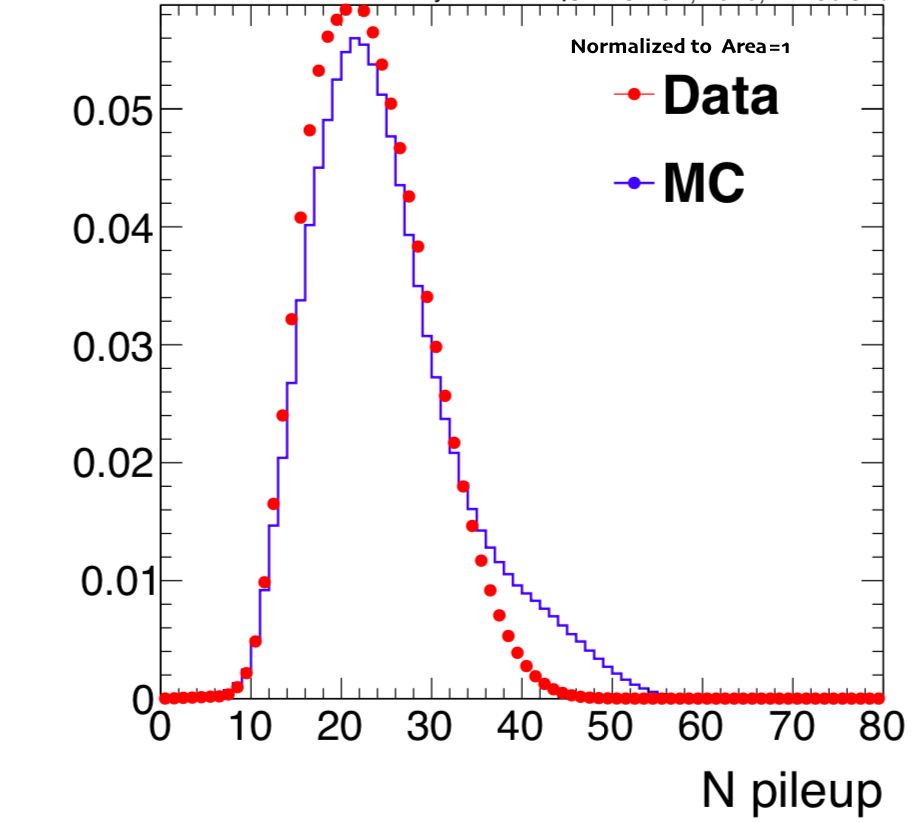
\includegraphics[width=0.45\linewidth]{figures/bg_Npileup.png}
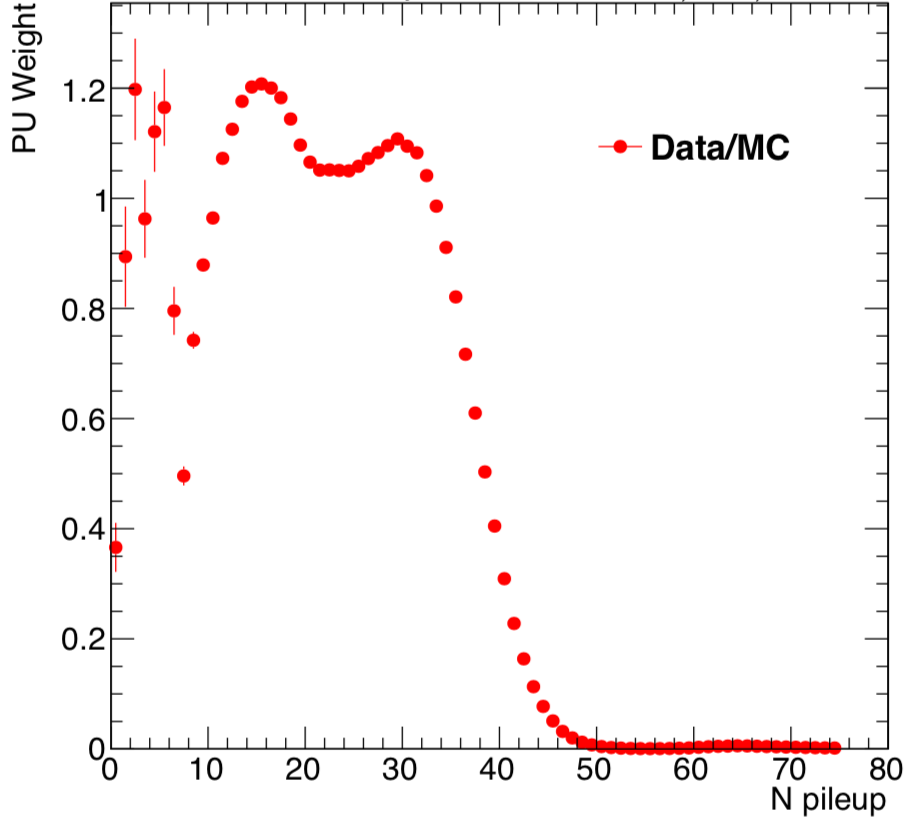
\includegraphics[width=0.45\linewidth]{figures/bg_pileupratio.png}
\caption{Pileup number profiles (left) for RunIISummer16 MC and 2016 data; and the pileup re-weighting function (right).}
\label{fig:bg_pileup}
\end{center}
\end{figure}

\section{Monte Carlo Efficiencies}
Weights are also applied to the MC samples in terms of the discrepancies in HLT and lepton ID/Iso efficiencies between data and MC samples. The probability of a lepton passing HLT, ID and Iso is:
\begin{align*}
P(HLT\cdot ID\cdot Iso) & = P(HLT|ID\cdot Iso)\times P(ID\cdot Iso) \\
 & = P(HLT|ID\cdot Iso)\times P(Iso|ID)\times P(ID),
\end{align*}
where $P(HLT\cdot ID\cdot Iso)$ denotes the efficiency of a lepton passing HLT, ID and Iso; $P(HLT|ID\cdot Iso)$ is the efficiency of a lepton passing HLT under the condition of it passing ID and ISO, and is also referred to as trigger efficiency; $P(ID\cdot Iso)$ is the combined ID/Iso efficiency; $P(Iso|ID)$ is the efficiency of a lepton passing Iso under the condition that it passes ID, referred to as the Iso efficiency; $P(ID)$ is the ID efficiency. The efficiencies are all calculated using a Tag-and-Probe method in this analysis, as discussed below. 

\subsection{Muon ID/Iso Efficiency}
The ID/Iso efficiencies may differ between MC and data due to imprecise modeling of detector performance. Therefore efficiencies are measured and scale factors (SF) are calculated for the MC samples to counter this effect. The Muon High $p_T$ ID, Tracker High $p_T$ ID and the Tracker Isolation efficiencies are measured separately using the tag-and-probe method described below. Events are selected from the SingleMuon dataset for data and DYJetsToLL\_M-50\_TuneCUETP8M1\_13TeV-madgraphMLM-pythia8 dataset for MC with pileup reweighting applied. 

\vspace{0.3cm}
In the tag-and-probe method, a tag muon and a probe muon are selected from an event. The tag muon is a muon required to be identified with high accuracy, which helps eliminate bias, and the probe muon is the muon candidate from which the efficiency is studied. A event is kept only if two muons are found with one passing the "tag" criteria while the other passing the "probe" criteria. For the muon ID/Iso efficiency measurement, the tag criteria are:
\begin{enumerate}
\item passing the \texttt{tight} Muon ID and the $relIso<0.2$ Iso requirement recommended by CMS Muon POG
\item passing \texttt{HLT\_IsoMu24} and $p_T > 26\GeV$
\end{enumerate}

The ID and Iso requirements ensure that the tag muon is a well defined muon. The \texttt{HLT\_IsoMu24} requirement is the un-prescaled HLT with lowest $p_T$ threshold in the SingleMuon dataset. Requiring the tag muon to pass this HLT assures that the selected event will be kept in the SingleMuon dataset so that the efficiencies to be measured for the probe muon would not be biased due to the dataset selection. The $p_T > 26\GeV$ requirement is added to enforce that the trigger is highly efficient for the tag muon. A muon candidate is considered as a probe if it is reconstructed as either a global muon or a tracker muon, with $p_T > 20$\GeV.

\vspace{0.3cm}
A known issue with the tracker system during Run Periods B to F caused some tracking inefficiency in the presence of heavily ionizing particles (HIPs). The effect on the muon reconstruction is found to be minor, and accounted for by calculating the efficiency in data for muons separately for Runs B to F and Runs G to H. And an additional 1\% uncertainty is assigned to cover the effect of the tracking inefficiency issue on the muon reconstruction. Considering 19.71 fb$^{-1}$ in run B to F and 16.15 fb$^{-1}$ in Run G to H, a flat random number between [0,1] is generated for each MC event, and if it is larger than $19.71$ fb$^{-1}/(19.71$ fb$^{-1}+16.15$ fb$^{-1})=0.5496$ the scale factors calculated from the muon efficiency in Run B to F would be assigned to the event, otherwise the SFs from Run GH are assigned.

\subsubsection{Muon ID Efficiency}
In the ID efficiency measurement, any muon candidate from the object reconstruction with $p_T > 20\GeV$ and $|\eta|<2.4$ (base muon selection in the analysis) could be considered as a probe muon. The invariant mass spectra of the tag-probe muon pairs are calculated for various $p_T - \eta$ bins, with each set including a spectrum for those pairs with probe muon passing the ID, while another spectrum for pairs with probe muon failing the ID. The invariant mass spectrum consists of $Z\rightarrow \mu\mu$ process and various background processes. The $Z\rightarrow \mu\mu$ events are considered signal and the probe muon in these events are true muons. In this case, the efficiency is calculated as
\begin{equation}
\epsilon=N_{signal}^{pass}/(N_{signal}^{pass}+N_{signal}^{fail}). 
\end{equation}
The spectra are fit into $signal+background$ models, and the integral of the signal shape is $N_{signal}^{pass}$ in the passing category and $N_{signal}^{fail}$ in the failing category for each bin. 

\vspace{0.3cm}
The signal function used for the fitting is the sum of 2 Voigtians. The background profile can either be RooCMSShape~\cite{bg_cmsshape} or a third order Chebychev polynomial. An example of the fitting plots is given in Figure~\ref{fig:bg_tnpmuonid}, for the Tracker High $p_T$ muon ID efficiency measurement.
\begin{figure}[htbp]
\begin{center}
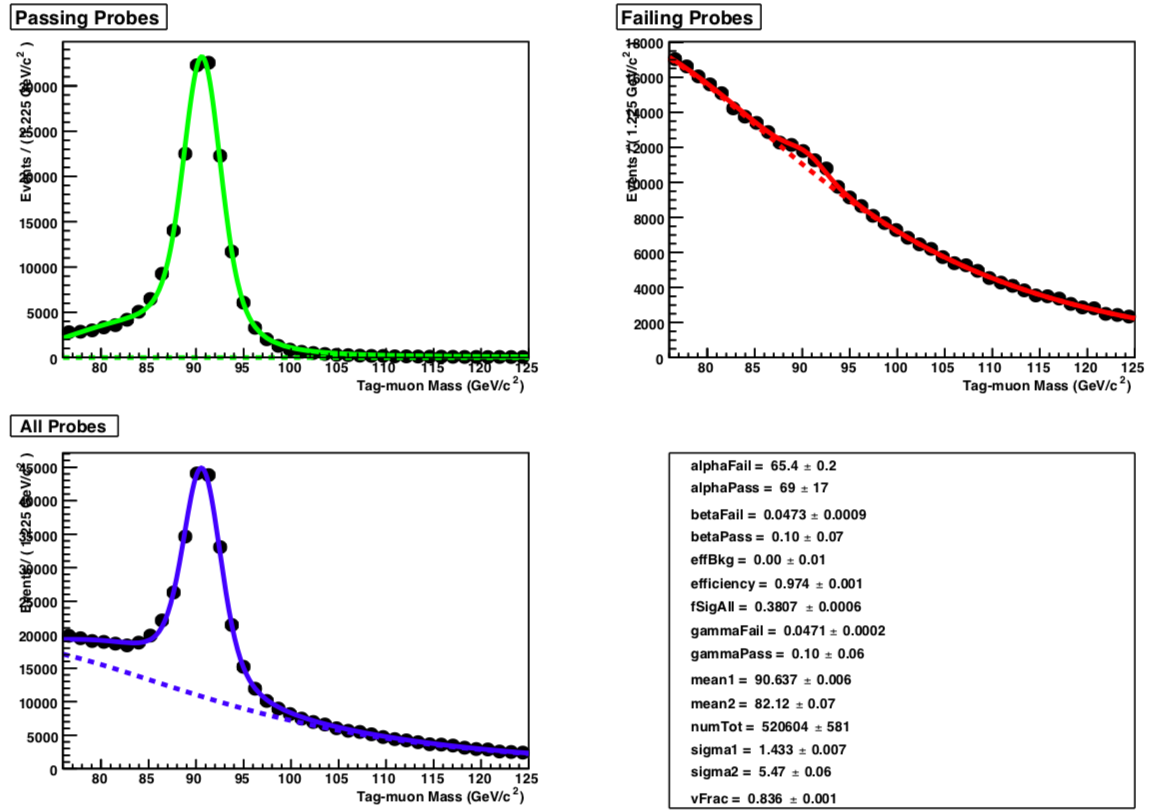
\includegraphics[width=0.9\linewidth]{figures/bg_tnpmuonid.png}
\caption{An example of the $\mu\mu$ invariant mass spectrum in one $p_T - \eta$ bin with the $signal+background$ fitting (solid lines) for the efficiency measurement of the Tracker High $p_T$ ID.} The dashed lines show the background contribution.
\label{fig:bg_tnpmuonid}
\end{center}
\end{figure}

\vspace{0.3cm}
Figures~\ref{fig:bg_muontkideff} to \ref{fig:bg_muonmcideff} show the efficiency results calculated from both Tracker High $p_T$ ID and High $p_T$ ID.

\begin{figure}[htbp]
\begin{center}
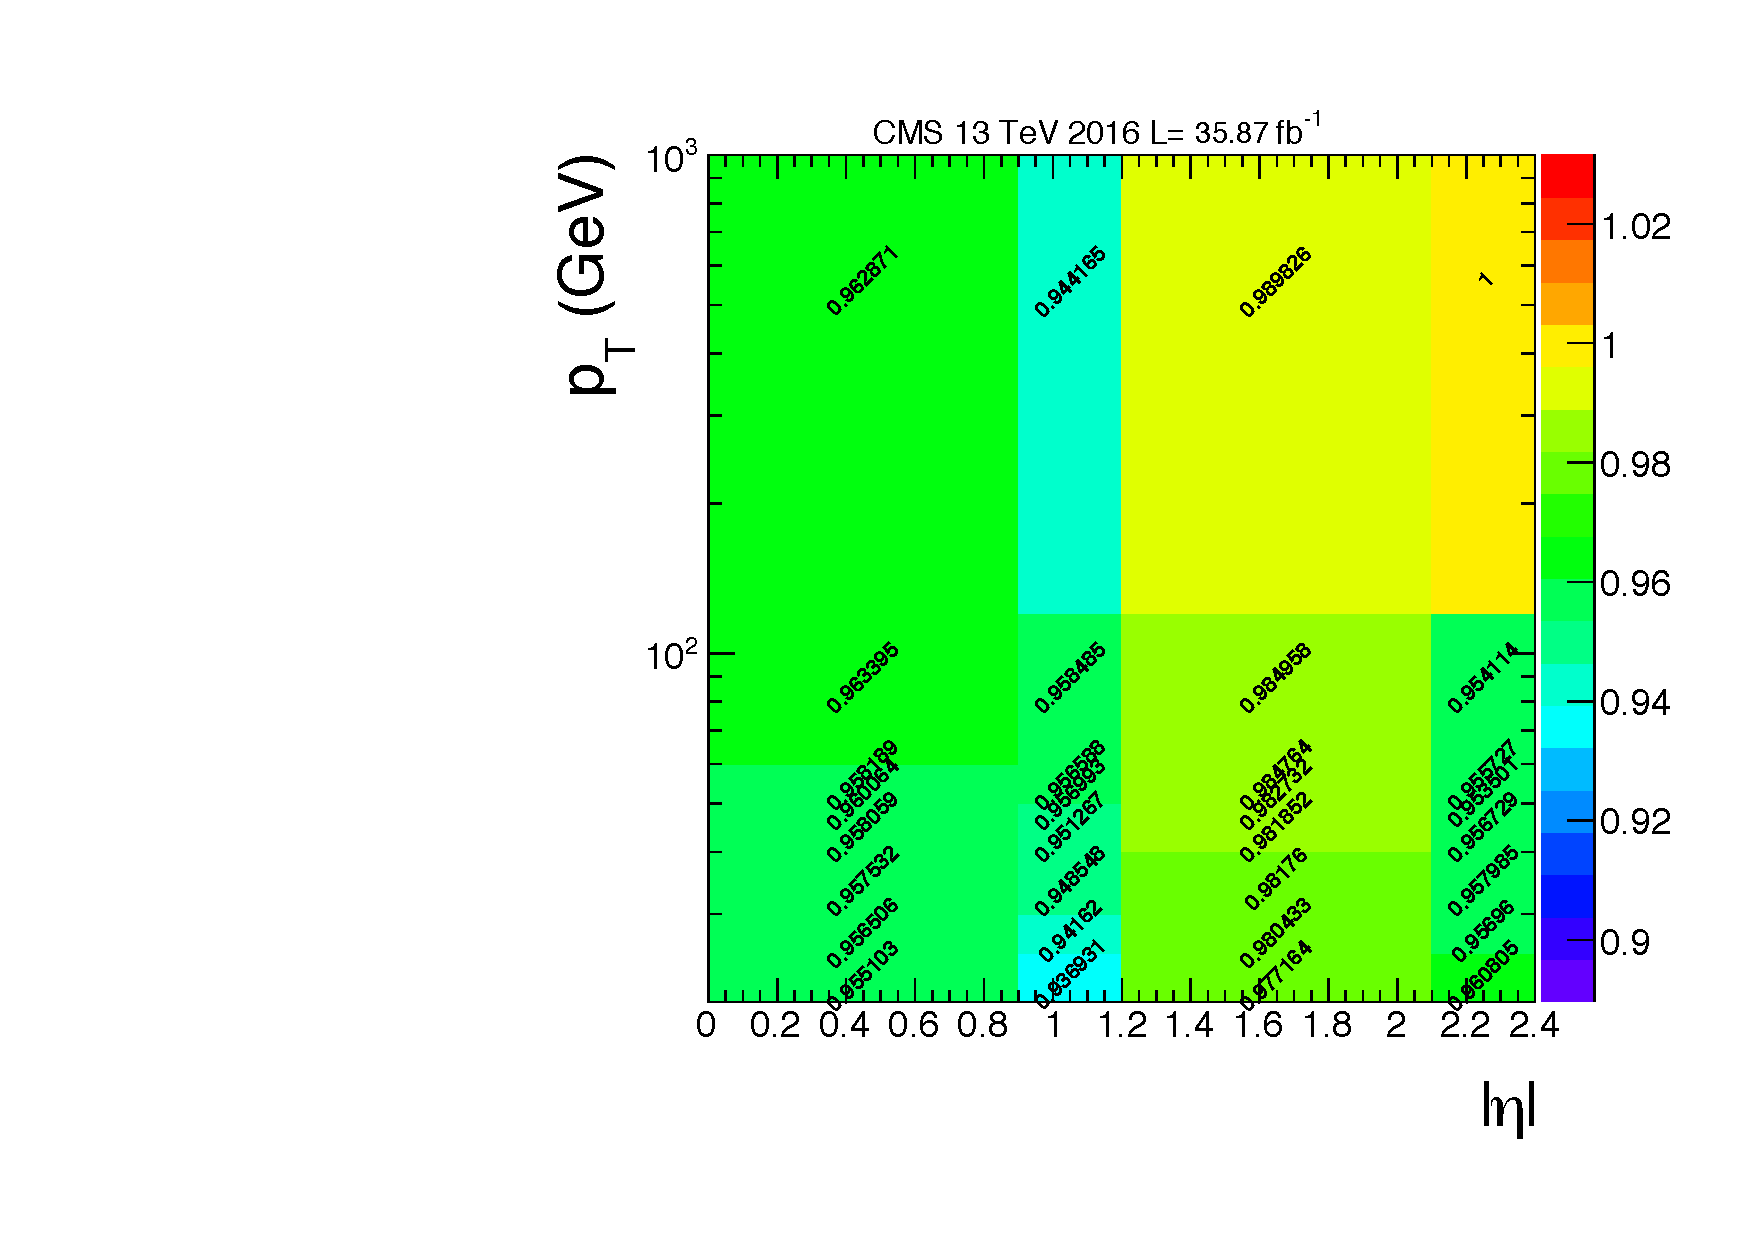
\includegraphics[width=0.49\linewidth, page=1]{figures/bg_muonidisoeff.pdf}
\includegraphics[width=0.49\linewidth, page=2]{figures/bg_muonidisoeff.pdf}
\caption{High $p_T$ Muon ID efficiency for 2016 ReReco data as a function of muon $p_T$ and $|\eta|$, for 2016 Run Peroids B--F (left) and 2016 G--H (right).}
\label{fig:bg_muontkideff}
\end{center}
\end{figure}

\begin{figure}[htbp]
\begin{center}
\includegraphics[width=0.49\linewidth, page=3]{figures/bg_muonidisoeff.pdf}
\includegraphics[width=0.49\linewidth, page=4]{figures/bg_muonidisoeff.pdf}
\caption{Tracker High $p_T$ Muon ID efficiency for 2016 ReReco data as a function of muon $p_T$ and $|\eta|$, for 2016 Run Peroids B--F (left) and 2016 G--H (right).}
\label{fig:bg_muonideff}
\end{center}
\end{figure}

\begin{figure}[htbp]
\begin{center}
\includegraphics[width=0.49\linewidth, page=5]{figures/bg_muonidisoeff.pdf}
\includegraphics[width=0.49\linewidth, page=6]{figures/bg_muonidisoeff.pdf}
\caption{Muon ID efficiency for RunIISummer16 MC as a function of muon $p_T$ and $|\eta|$, for High $p_T$ Muon ID (left) and Tracker High $p_T$ Muon ID (right).}
\label{fig:bg_muonmcideff}
\end{center}
\end{figure}

\vspace{0.3cm}
Because the Tracker High $p_T$ ID is a loosened version of the High $p_T$ ID, if a muon passes the High $p_T$ ID, it will also pass the Tracker High $p_T$ ID. The muon ID scale factor for an event is therefore calculated as:
\begin{small}
\begin{align*}
SF & =\epsilon^{data}/\epsilon^{MC} \\
 & =\frac{(\epsilon_{HighPt}(\mu_1)\times \epsilon_{trkHighPt}(\mu_2)+\epsilon_{trkHighPt}(\mu_1)\times \epsilon_{HighPt}(\mu_2)-\epsilon_{HighPt}(\mu_1)\times \epsilon_{HighPt}(\mu_2))_{data}}{(\epsilon_{HighPt}(\mu_1)\times \epsilon_{trkHighPt}(\mu_2)+\epsilon_{trkHighPt}(\mu_1)\times \epsilon_{HighPt}(\mu_2)-\epsilon_{HighPt}(\mu_1)\times \epsilon_{HighPt}(\mu_2))_{MC}}
\end{align*}
\end{small}

\subsubsection{Muon Iso Efficiency}
The muon tracker isolation efficiency is also measured using the tag-and-probe method, with an additional requirement on the probe muon to pass the tracker High $p_T$ ID. Because the tracker isolation selection applies to both muons, the ratio between the efficiencies of data and MC is used as the MC scale factor for the isolation. The SF values versus $p_T$ and $\eta$ are shown in Figure~\ref{fig:bg_muonisosf}
\begin{figure}[htbp]
\begin{center}
\includegraphics[width=0.49\linewidth, page=7]{figures/bg_muonidisoeff.pdf}
\includegraphics[width=0.49\linewidth, page=8]{figures/bg_muonidisoeff.pdf}
\caption{\texttt{tracker ISO} data/MC efficiency scale factors as a function of muon $p_T$ and $|\eta|$, for 2016 Run Peroids B--F (left) and 2016 G--H (right).}
\label{fig:bg_muonisosf}
\end{center}
\end{figure}

\subsection{Electron ID/Iso Efficiency}
Based on the recommendation from the CMS EGamma POG, the \texttt{Loose} cut-based identification (ID) selection is required for all the electron candidates. Because a PF isolation is already included in the \texttt{Loose} ID, no additional electron isolation is needed.

\vspace{0.3cm}
The electron \texttt{Loose} ID (including PF ISO) efficiency and scale factors are provided by the EGamma POG, measured by the tag-and-probe method. Figure~\ref{fig:bg_eidsf} shows the electron \texttt{Loose} ID scale factors used in this analysis. The electron reconstruction is also affected by the tracking inefficiency issue, the reconstruction scale factors are also provided by the EGamma POG to counter this effect. Figure~\ref{fig:bg_gsfsf} shows the electron reconstruction scale factors from EGamma POG used in this analysis.  

\begin{figure}[htbp]
\centering
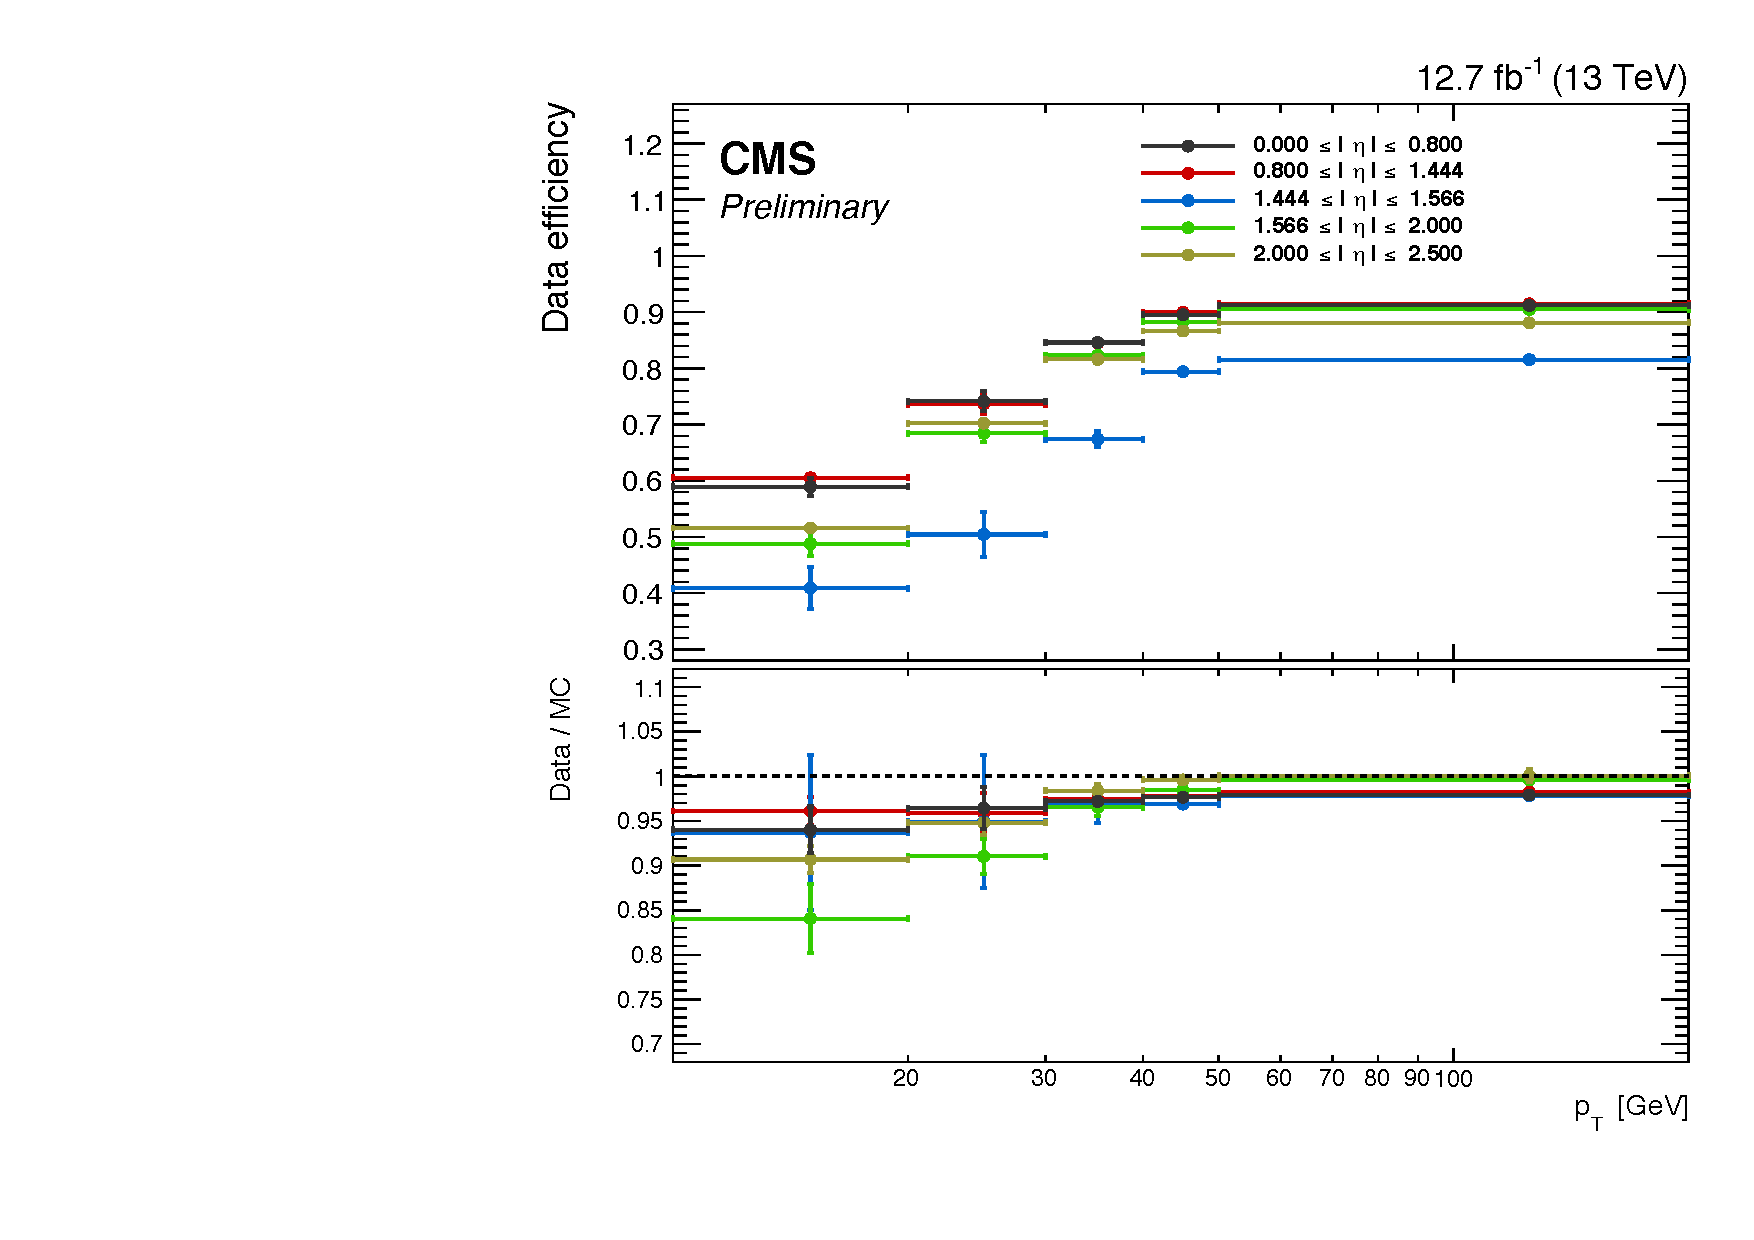
\includegraphics[width=0.66\linewidth, page=1]{figures/bg_elooseideff.pdf}
\includegraphics[width=0.66\linewidth, page=2]{figures/bg_elooseideff.pdf}
\caption{EGamma POG electron \texttt{Loose} ID (including pf Iso) efficiency scale factors for 2016 dataset analysis.}
\label{fig:bg_eidsf}
\end{figure}

\begin{figure}[htbp]
\centering
\includegraphics[width=0.66\linewidth, page=2]{figures/bg_erecoeff.pdf}
\caption{EGamma POG electron reconstruction scale factors for 2016 dataset analysis.}
\label{fig:bg_gsfsf}
\end{figure}

\subsection{Trigger Efficiency}\label{sec:bkg_trig}
The HLT is designed for making fast decisions for accepting data, and therefore the reconstruction of objects' properties at the HLT level are not as precise compared to the offline reconstruction. Trigger efficiency studies for offline objects are important to physics analyses in two regards: to suppress the trigger efficiency effect on the data by optimizing data selection; and to compensate the discrepancy in terms of trigger efficiency between data and simulation samples by applying trigger efficiency SFs to MC samples.
\subsubsection{SingleMuon HLT Efficiency}
For the muon channel selection, events are required to pass the single muon HLT requirement of either \texttt{HLT\_Mu50} or \texttt{HLT\_TkMu50}. The combined trigger efficiencies and SFs are centrally derived by the Muon POG, measured with the tag-and-probe method. The summary plots in Figure~\ref{fig:bg_trgeff_mu} show the trigger efficiencies versus $p_T$ (left) and $\eta$ (right). In the $p_T$ plot, a rising edge of the efficiency can be clearly seen around the $p_T$ threshold of the HLT. To avoid events falling on the rising edge in the trigger efficiency, leading to greater difficulty in the background modeling, the $p_T$ of the leading muon is required to be at least 60\GeV.

\begin{figure}[htpb]
\begin{center}
\includegraphics[width=0.49\linewidth, page=2]{figures/bg_muontrgeff.pdf}
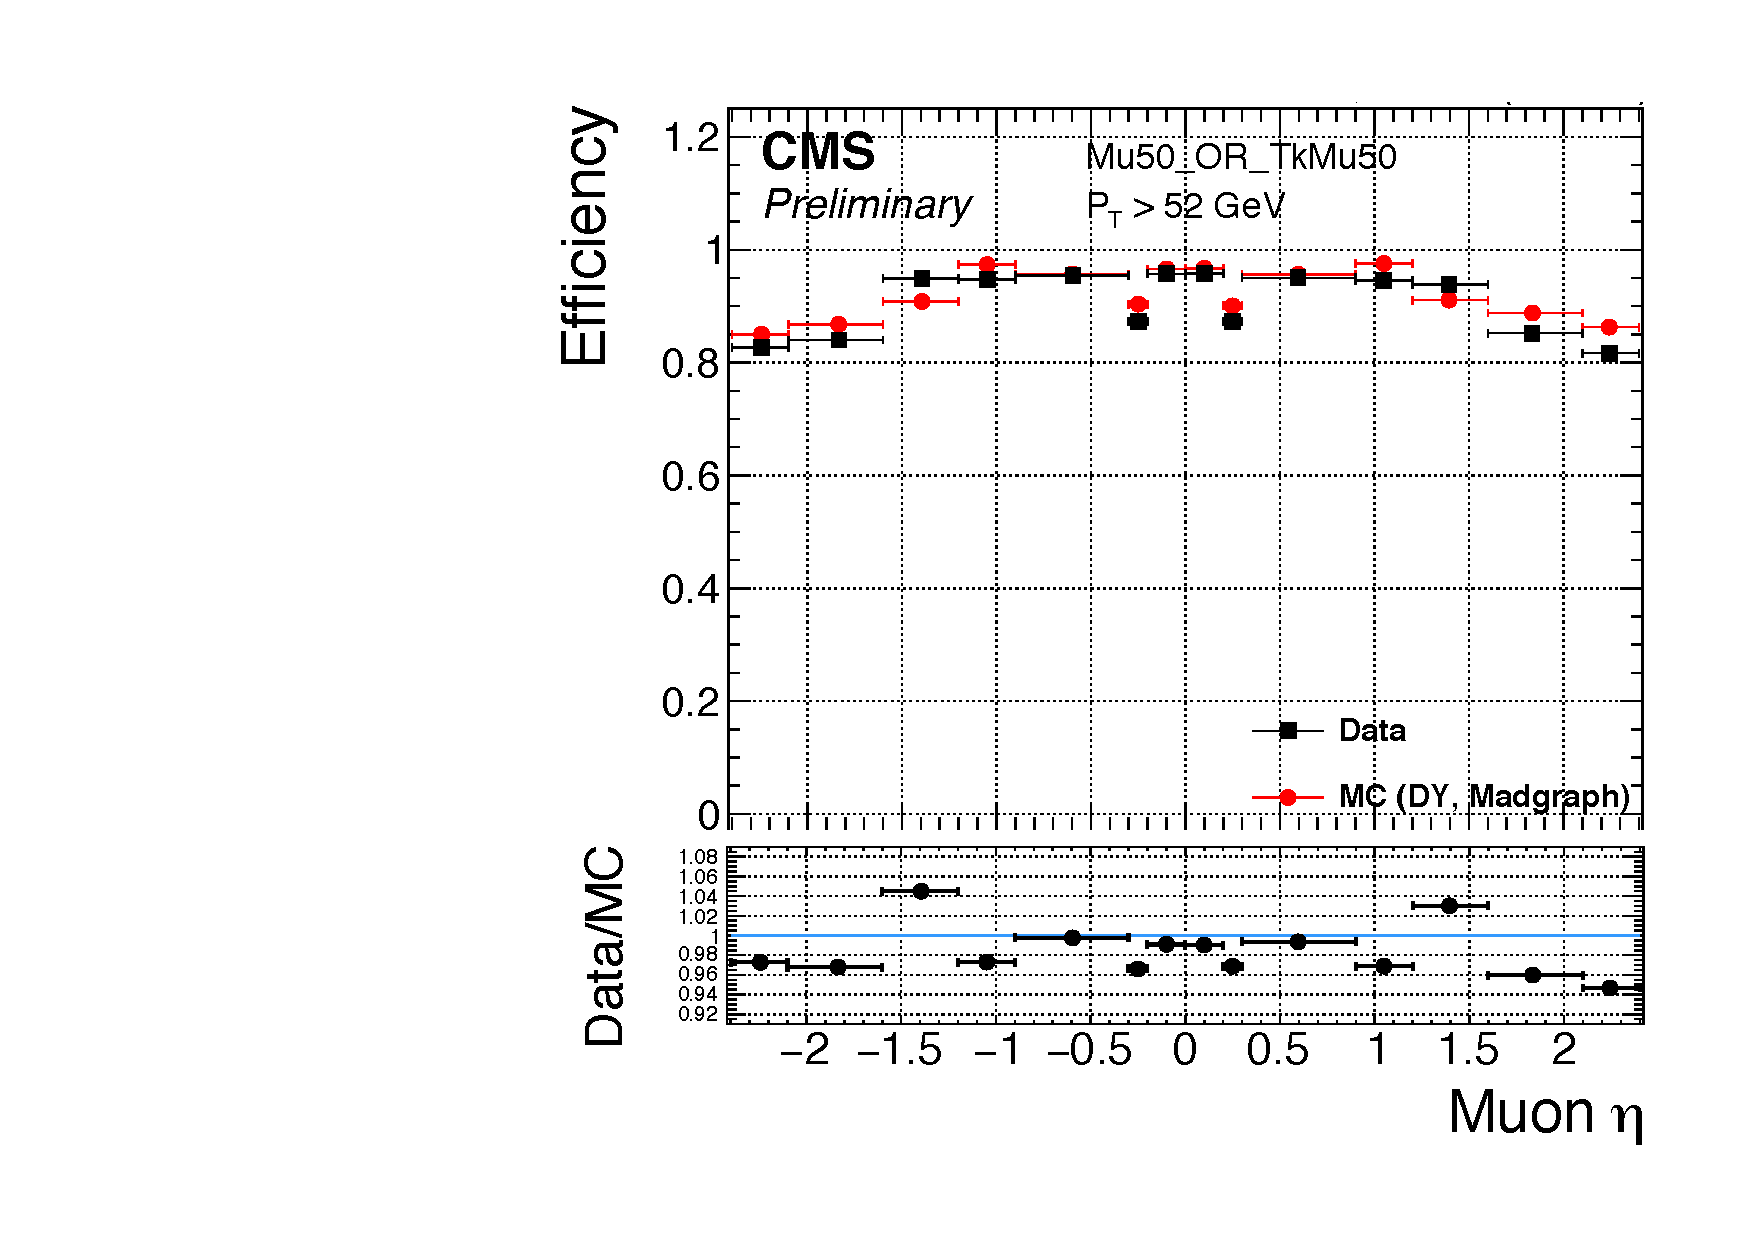
\includegraphics[width=0.49\linewidth, page=1]{figures/bg_muontrgeff.pdf}
\caption{Muon trigger efficiency for 2016 data and MC, versus $p_T$ (left) and $\eta$ (right)}
\label{fig:bg_trgeff_mu}
\end{center}
\end{figure}

\vspace{0.3cm}
The efficiency results are delivered in the form of 2D histograms in $p_T - \eta$. The calculated ratio of efficencies between data and MC are applied to the leading muon of the pair in the MC events only as the trigger efficiency scale factor, considering that number of events in either data or MC is negligible with the subleading muon passing the HLT while leading muon fails the selection.

\subsubsection{SingleElectron HLT Efficiency}
The SingleElectron HLT (\texttt{HLT\_Ele115\_CaloIdVT\_GsfTrkIdT}) efficiency is measured for data and MC using the tag-and-probe method. Events are selected from the SingleElectron dataset in data and the DYJetsToLL\_M-50\_ TuneCUETP8M1\_13TeV-amcatnloFXFX-pythia8 dataset for MC with pileup reweighting. The "tag" criteria are:
\begin{enumerate}
\item passing the \texttt{tight} cut-based identification (ID) and isolation (Iso) recommended by the EGamma POG %shown in Table~\ref{tab:electron-tightid}
\item passing \texttt{HLT\_Ele27\_WPTight\_Gsf} with $p_T>30$ and $|\eta|<2.1$
\end{enumerate}

%\begin{table}[htb!]
%  \center
%  \caption{The cuts used in the POG \texttt{tight} electron identification.}
%  \label{tab:electron-tightid}
%  \begin{tabular}{r c c c}
%    \hline
%    Variable & Barrel & Endcap \\
%    \hline
%    $|\eta_{\rm SC}|$ acceptance & $(0, 1.479)$ & $(1.479, 2.5)$\\
%    $\sigma_{i\eta,i\eta} <$ & 0.00998  & 0.0292 \\
%    $|\Delta\eta_{in}| <$ & 0.00308  & 0.00605 \\
%    $\Delta\phi_{in} <$ & 0.0816  & 0.0394 \\
%    \texttt{hOverE} $<$ & 0.0414  & 0.0641 \\
%    \texttt{relIsoWithEA} $<$ & 0.0588  & 0.0571 \\
%    $|1/E - 1/p| <$ & 0.0129  & 0.0129 \\
%    expectedMissingInnerHits $\leq$ & 1  & 1 \\
%    conversion veto & yes  & yes \\
%    \hline
%  \end{tabular}
%\end{table}

The criterion of \texttt{tight} ID/Iso ensures the tag electron to be a well identified electron. The \texttt{HLT\_Ele27\_WPTight\_Gsf} is the un-prescaled HLT with lowest $p_T$ threshold in the SingleElectron dataset. This requirement ensures that the trigger efficiency to be measured from the probe electron is not biased due to the dataset for selection. A electron is considered as a probe if it satisfies the condition of the trigger efficiency measurement, which is passing the \texttt{loose} ID/Iso in this analysis, as described in Section~\ref{sec:ob_eidiso}.

\vspace{0.3cm}
The electron trigger efficiencies are measured as a function of the reconstructed electron $p_T$ and $|\eta|$ for both the 2016 full dataset and RunIISummer16 MC. Figure~\ref{fig:bg_etrgtnp} gives an example of invariant mass spectrum of the electron pair. Because only electrons passing ID/Iso criteria are selected, the background fraction is very small for the trigger efficiency measurement.

\begin{figure}[htpb]
\begin{center}
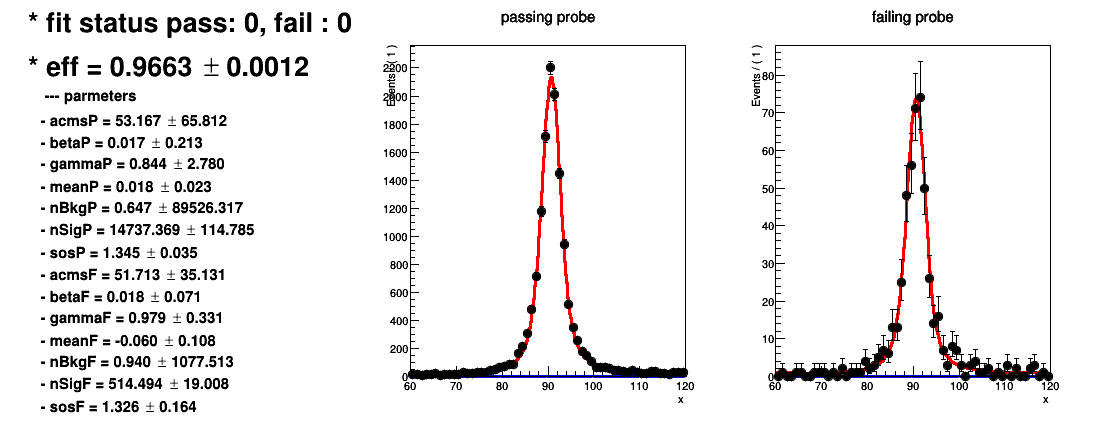
\includegraphics[width=0.95\linewidth, page=1]{figures/bg_etrgtnp.png}
\caption{An example of one  $p_T - |\eta|$ bin of the electron pair invariant mass spectrum with the $signal+background$ fit for the efficiency measurement of \texttt{HLT\_Ele27\_WPTight\_Gsf}. The background component shown by the blue line is negligible due to the ID/Iso criteria on the probe electron.}
\label{fig:bg_etrgtnp}
\end{center}
\end{figure}

\vspace{0.3cm}
The measured efficiencies are shown in Figures ~\ref{fig:trgeff_el_dt} and \ref{fig:trgeff_el_mc} for data and MC respectively. The corresponding Data/MC scale factors are shown in Figure~\ref{fig:trgeff_el_sf}. Similar to the muon channel, the SingleElectron HLT efficiency SF is applied on the leading electron in the MC samples as reweighting factors to model the electron trigger efficiency, and a $p_T > 120$\GeV selection is added to the leading electron.

\begin{figure}[htpb]
\begin{center}
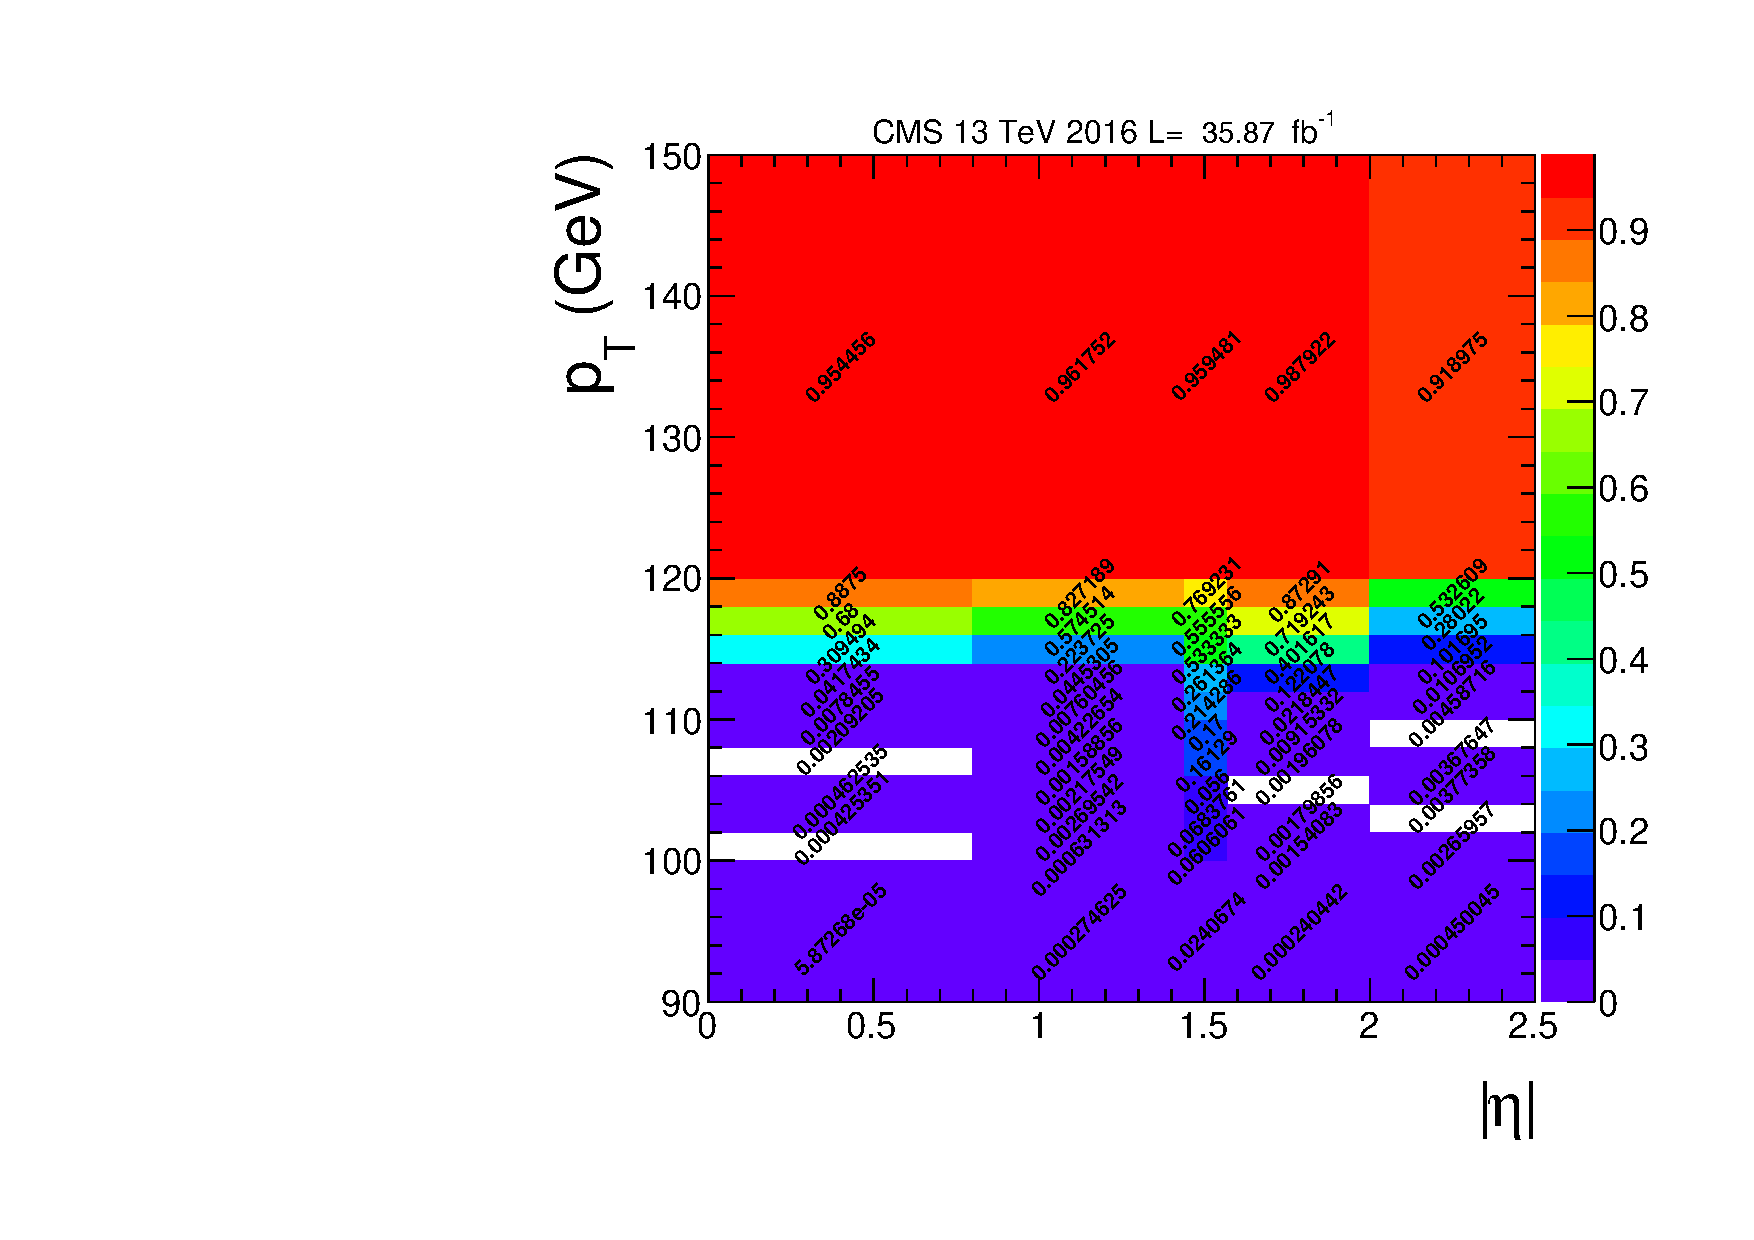
\includegraphics[width=0.49\linewidth, page=1]{figures/hlt115electron_2016fulleff_absetapt.pdf}
\includegraphics[width=0.49\linewidth, page=2]{figures/hlt115electron_2016fulleff_absetapt.pdf}
\caption{Electron trigger efficiency from 2016 ReReco dataset as a function of reconstructed electron $p_T$ and $|\eta|$. Left for $p_T <150\GeV$, right for $p_T >150\GeV$. }
\label{fig:trgeff_el_dt}
\end{center}
\end{figure}

\begin{figure}[htpb]
\begin{center}
\includegraphics[width=0.49\linewidth, page=3]{figures/hlt115electron_2016fulleff_absetapt.pdf}
\includegraphics[width=0.49\linewidth, page=4]{figures/hlt115electron_2016fulleff_absetapt.pdf}
\caption{Electron trigger efficiency from RunIISummer16 MC as a function of reconstructed electron $p_T$ and $|\eta|$. Left for $p_T <150\GeV$, right for $p_T >150\GeV$. }
\label{fig:trgeff_el_mc}
\end{center}
\end{figure}

\begin{figure}[htpb]
\begin{center}
\includegraphics[width=0.49\linewidth, page=5]{figures/hlt115electron_2016fulleff_absetapt.pdf}
\includegraphics[width=0.49\linewidth, page=6]{figures/hlt115electron_2016fulleff_absetapt.pdf}
\caption{Electron trigger efficiency Data/MC scale factors as a function of reconstructed electron $p_T$ and $|\eta|$. Left for $p_T <150\GeV$, right for $p_T >150\GeV$. }
\label{fig:trgeff_el_sf}
\end{center}
\end{figure}

\clearpage
\section{\boldmath{\Zjets} Background Modeling}\label{sec:dybk}
In this analysis data-driven background modeling methods are used for the majority of the backgrounds, including the \Zjets background. The data-driven method in this analysis has benefits in that:
\begin{enumerate}
\item The number of available MC events in the high energy region is limited, while the data-driven method offers more statistics in our region of interest.
\item The modeling of \ptmiss for the signal region is more reliable in the data-driven background methods, considering that detector conditions and pileup modeling may be imperfect in MC.
\end{enumerate}

As Figures~\ref{fig:mc_nvtx} and \ref{fig:mc_rho} show, even with the pileup reweightings applied, the vertex multiplicity and $\rho$ (a parameter describing the pileup energy in the detector) distributions are still not precisely reproduced by MC.
\begin{figure}[htbp!]
\centering
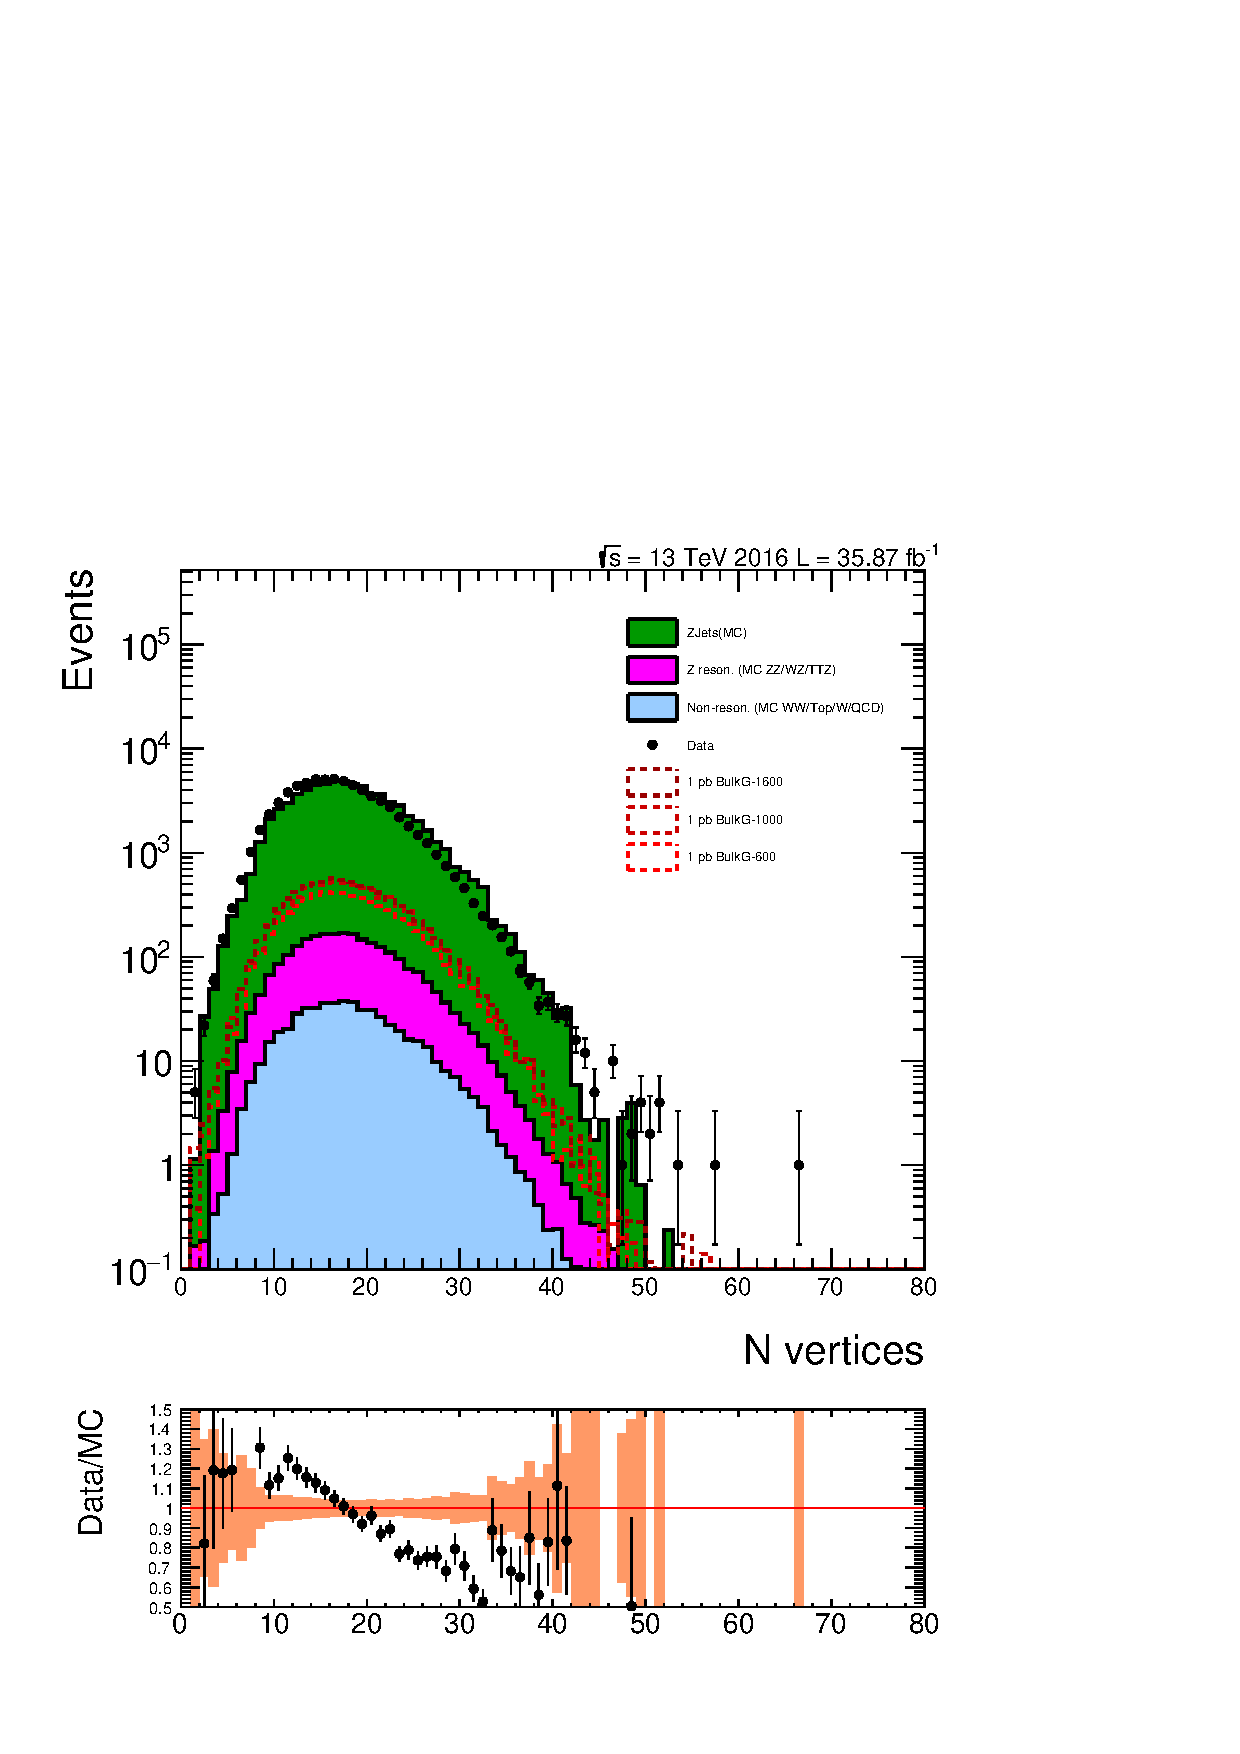
\includegraphics[width=0.46\linewidth, page=1]{figures/ReMiniSummer16_MC_GMCPhPtWt_tightzpt50_puWeightsummer16_metfilter_unblind_el_log_1pb.pdf}
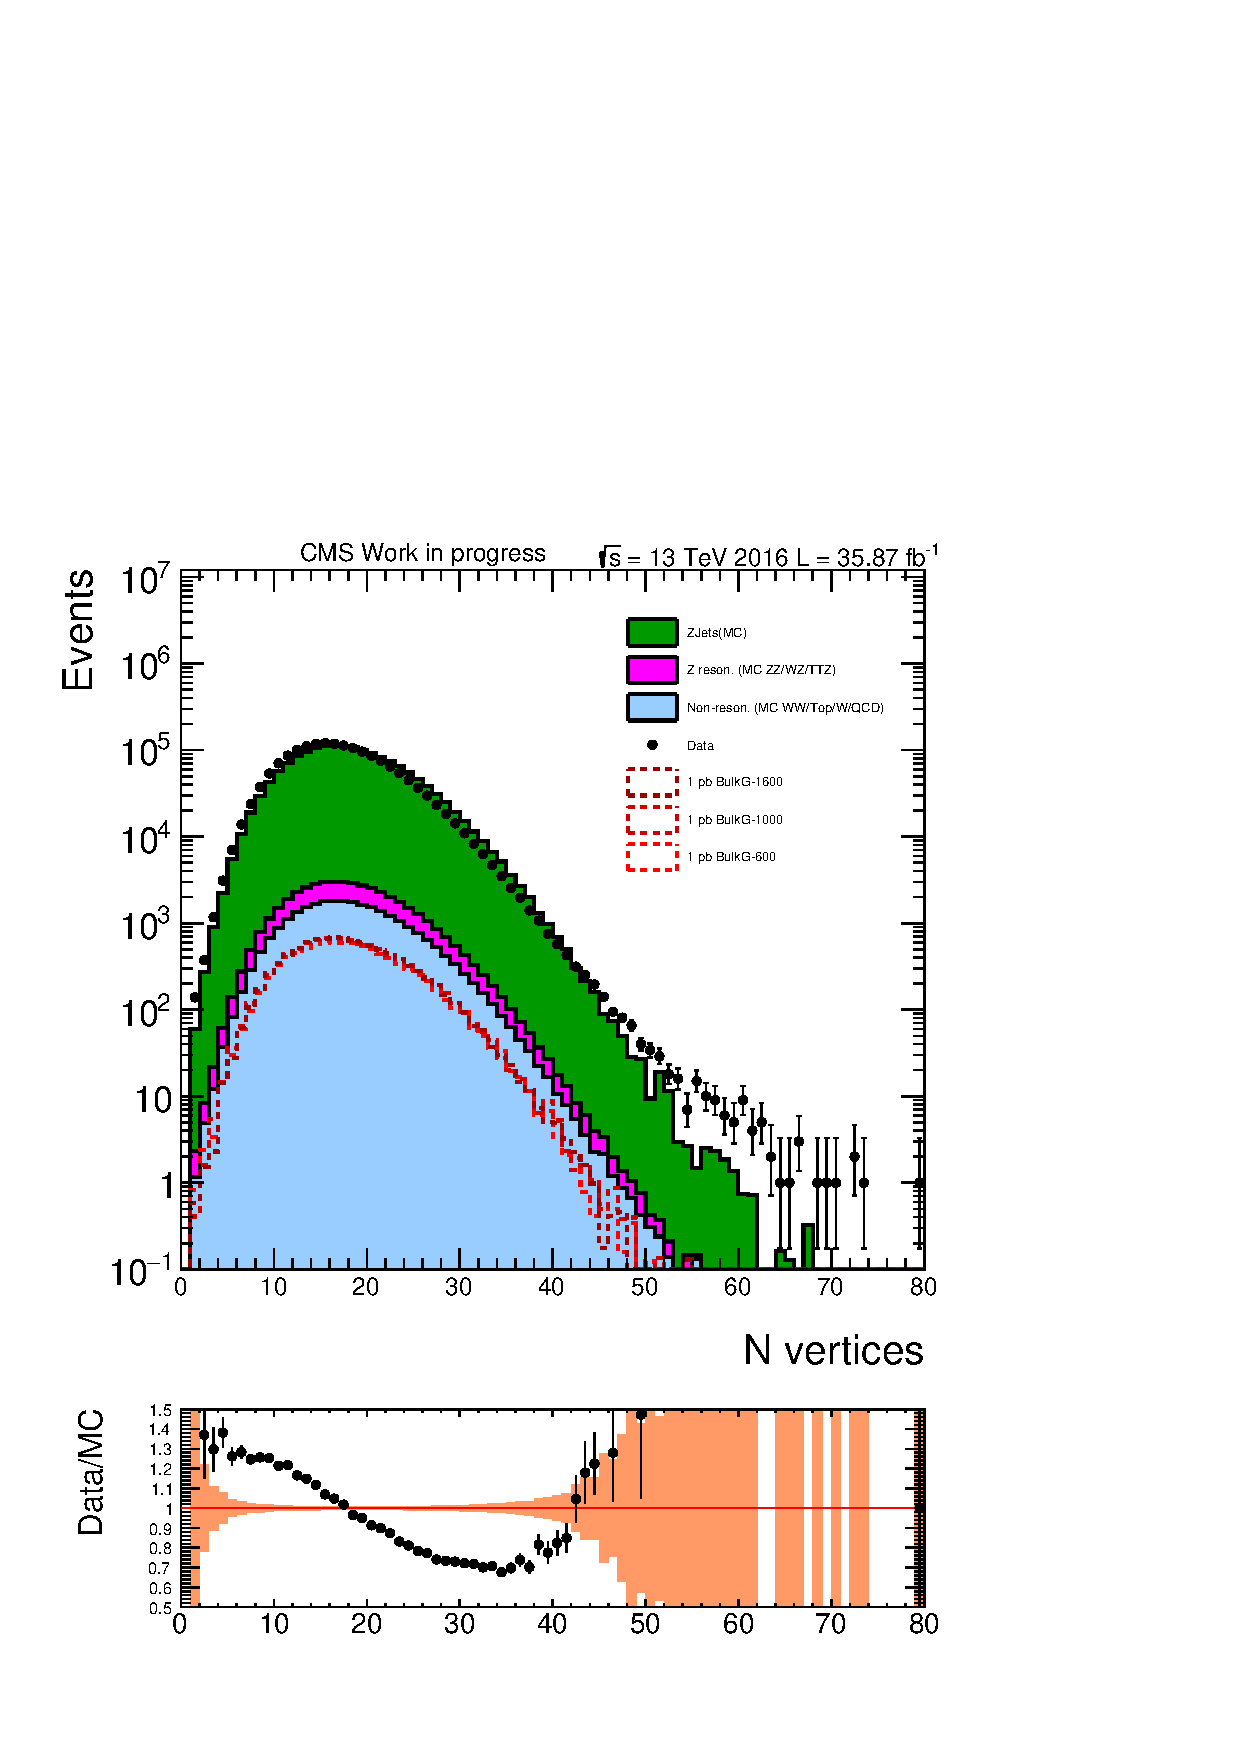
\includegraphics[width=0.46\linewidth, page=1]{figures/ReMiniSummer16_MC_GMCPhPtWt_tightzpt50_puWeightsummer16_metfilter_unblind_mu_log_1pb.pdf}
\caption{Number of reconstructed vertices for electron (left) and muon (right) channels comparing data and MC.}
\label{fig:mc_nvtx}
\end{figure}

\begin{figure}[htbp!]
\centering
\includegraphics[width=0.46\linewidth, page=2]{figures/ReMiniSummer16_MC_GMCPhPtWt_tightzpt50_puWeightsummer16_metfilter_unblind_el_log_1pb.pdf}
\includegraphics[width=0.46\linewidth, page=2]{figures/ReMiniSummer16_MC_GMCPhPtWt_tightzpt50_puWeightsummer16_metfilter_unblind_mu_log_1pb.pdf}
\caption{The $\rho$ distributions for electron (left) and muon (right) channels comparing data and MC.}
\label{fig:mc_rho}
\end{figure}

\vspace{0.3cm}
The \Zjets background is characterized by a transversely boosted Z boson and a hadronic recoil balancing the momentum of the Z boson. The observed \ptmiss in this background is primarily instrumental. The \gjets events have a similar kinematic signature as \Zjets events, and can be used to model the \Zjets background in a data-driven way. This \gjets data-driven approach is prefered over the MC background modeling because the \gjets sample offers more statistics in our regions of interest and the \ptmiss reconstruction is more reliable in the \gjets data than the MC samples. As the signal process can not contribute to the \gjets data, it is safe to use the \gjets data for the background modeling.

\vspace{0.3cm}
The ultimate goal is to use the \gjets events to model the $m_T$ distribution of the \Zjets background. According to Equation~\ref{eqn:intro_MTalt}, $m_T$ is determined by $m_{\ell\ell}$, ${p}_{T}^{\ell\ell}$, ${p_{T}}^{miss}_\parallel$ and ${p_{T}}^{miss}_\perp$, where $m_{\ell\ell}$ is the invariant mass of the lepton pair; ${p}_{T}^{\ell\ell}$ is the $\vec p_T$ sum of the lepton pair; ${p_{T}}^{miss}_\parallel$ refers to the projection of \ptmiss in the direction of ${p}_{T}^{\ell\ell}$ and ${p_{T}}^{miss}_\perp$ is the portion perpendicular to ${p}_{T}^{\ell\ell}$. It is crucial to model $m_{\ell\ell}$, ${p}_{T}^{\ell\ell}$, ${p_{T}}^{miss}_\parallel$ and ${p_{T}}^{miss}_\perp$ well. The workflow of the \Zjets data-driven modeling can be summerized as below and will be discussed in the following sections:
\begin{itemize}
\item \textbf{photon data cleaning}
\begin{itemize}
\item \gjets Event Selection in Section~\ref{sec:bg_gjetsel}
\item \gjets HLT Prescale Reweighting in Section~\ref{sec:bg_gjetHLT}
\item Physical \ptmiss Subtraction in Section~\ref{sec:bg_gjetphysmet}
\end{itemize}
\item \textbf{${p}_{T}^{\ell\ell}$ correction for photon data}
\begin{itemize}
\item ${p_T}^{\gamma}$ to ${p_T}^Z$ Reweighting in Section~\ref{sec:bg_gjetpt}
\end{itemize}
\item \textbf{$m_{\ell\ell}$ correction for photon data}
\begin{itemize}
\item Photon Mass Generation in Section~\ref{sec:gjetm}
\end{itemize}
\item \textbf{${p_{T}}^{miss}_\parallel$ and ${p_{T}}^{miss}_\perp$ corrections for photon data}
\begin{itemize}
\item \ptmiss Hadronic Recoil Tuning in Section~\ref{sec:gjetmet}
\end{itemize}
\end{itemize}

\subsection{\boldmath{\gjets} Event Selection}\label{sec:bg_gjetsel}
The \gjets events are selected from the SinglePhoton dataset with HLT \texttt{HLT\_Photon``PT''\_R9Id90\_HE10\_IsoM}, for \texttt{PT} = 22, 30, 36, 50, 75, 90, 120, 165\GeV. The \texttt{Loose} Photon ID defined and recommended by the CMS EGamma POG is applied. Furthermore, MET filters listed in Section~\ref{sec:metfilter} are also required in the photon data selection.

\vspace{0.3cm}
Even with the \texttt{Loose} Photon ID applied, the photon samples are still contaminated by many fake photons from sources such as ECAL APD spikes, ECAL noise that has not been flagged, and beam halo particles. Therefore, additional selections are applied as listed below:
\begin{itemize}
\item Only one reconstructed photon in the event. 
%\item Additional fake photon events cleansing  $i\eta- i\phi$ ($ix-iy$) filter maps as shown on Figure~\ref{fig:gjets_photon_clean_eta_phi_map}. Notice that the entire region around $\phi=0$, and $\pi$ in the $x-z$ plain on the ECAL Endcap are flagged out, where beam halo photons are dominant.
\item A cleansing filter applied based on problematic ECAL channel maps.
\item \texttt{sigmaIetaIeta}$>0.001$
\item \texttt{sigmaIphiIphi}$>0.001$  
\item ``Swiss Cross'':  $S = (1-E4/E1)<0.95$ , where $E1$ is the seed crystal energy, $E4$ is the sum of the energies in up, down, left and right crystals adjacent to the seed crystal.
\item ECAL seed crystal timing :   $t_0-1.5 ns < time < t_0+1.5 ns$, where $t_0$ is the peak time position. 
\item Minimum ionizing particle (MIP) total energy $< 4.9$\GeV to suppress halo induced showers in the ECAL.
\item Lepton veto: remove events with one or more reconstructed electrons with $ p_T > 10$\GeV, 
also remove events with jets containing more than 10\GeV of lepton energy.
This is to filter out processes such as $Z\to ee$ events, with one electron mis-identified as the photon. 
\end{itemize}

In addition, analogous to the Z boson preselection, $p_T ^{\gamma} > 50\GeV$ is applied in the photon data selection.

\subsection{\boldmath{\gjets} HLT Prescale Reweighting}\label{sec:bg_gjetHLT}
Both the L1T and HLT can be prescaled in order to suppress the very high rate low energy events. For the HLTs used in the \gjets event selection:
\texttt{HLT\_Photon<$p_T$>\_R9Id90\_HE10\_IsoM}, \\
 for $p_T$ = 22, 30, 36, 50, 75, 90, 120,165\GeV, prescales are applied as follows:
\begin{itemize}
\item $p_T$ threshold = 165\GeV: not pre-scaled, 
\item $p_T$ threshold = 50, 75, 90, and 120\GeV:  pre-scaled at only HLT.  
\item $p_T$ threshold = 22, 30, 36\GeV: pre-scaled at both L1T and HLT, 
\end{itemize}

For photon triggers with $p_T$ of 50\GeV and higher, the L1T prescale has no effect on our selected data. The HLT prescale factor is obtained from the trigger conditions information stored for the CMS data, and applied as a weight to correct the effect of the HLT prescale on the $p_T$ spectrum of the photons. Figure~\ref{fig:photon_pt_prescale} shows the photon $p_T$ spectrum with and without corrections for the HLT prescales.


\begin{figure}[htbp]
\begin{center}
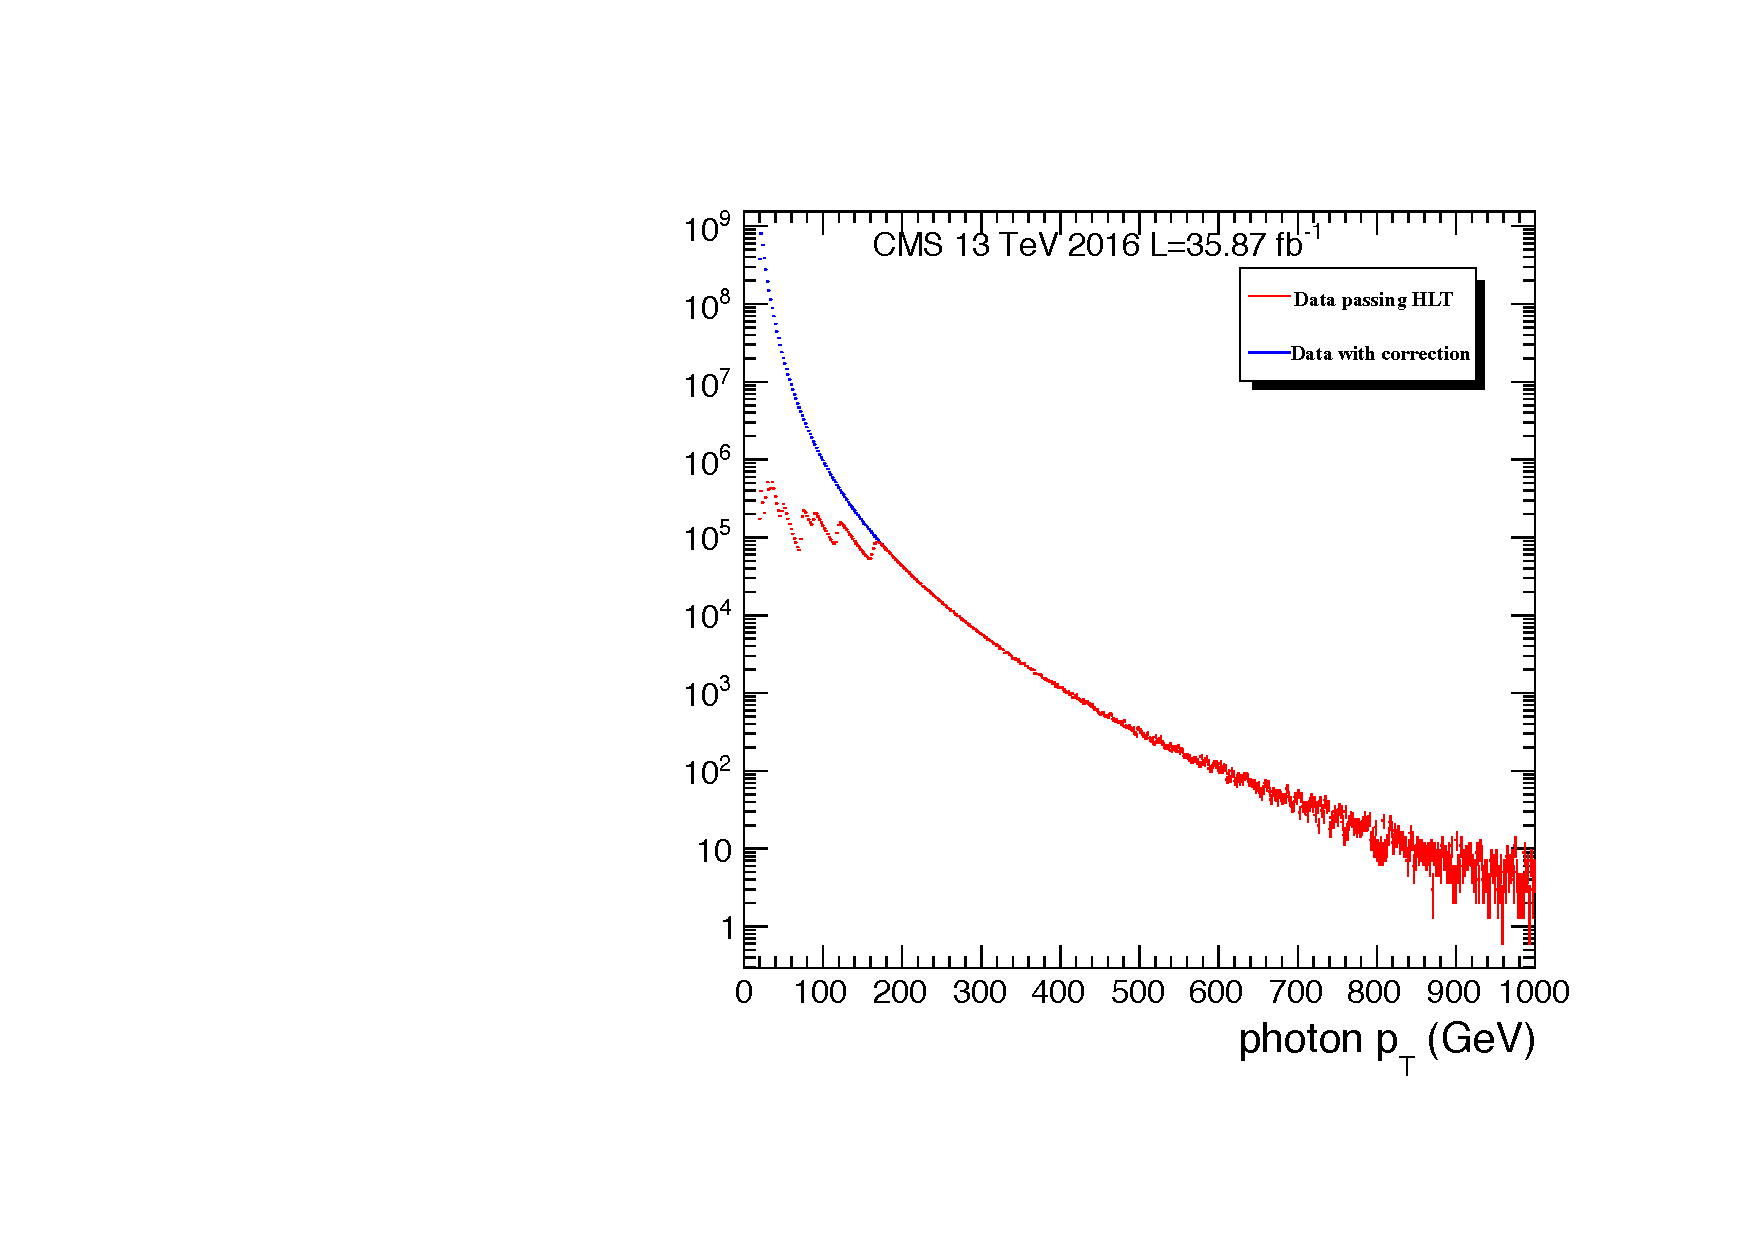
\includegraphics[width=0.86\linewidth]{figures/bg_photonHLT_reweight.pdf}
\caption{Photon $p_T$ distributions with and without the HLT prescale correction. }
\label{fig:photon_pt_prescale}
\end{center}
\end{figure}

\subsection{Physical \boldmath{\ptmiss} Subtraction}\label{sec:bg_gjetphysmet}
Like the \Zjets process, the \ptmiss in the process of \gjets is due to instrumental effects. However, processes like $W\gamma\rightarrow\ell\nu\gamma$ with physical \ptmiss can also contribute to the SinglePhone dataset. To model the kinematics of the \gjets process better, events with physical \ptmiss are subtracted from the SinglePhoton dataset using MC. MC samples shown in Table~\ref{tab:bg_photonMC} are used to describe the single photon dataset. Figures~\ref{fig:pho_met} and \ref{fig:pho_metpara} show the comparisons of the SinglePhoton data and MC for 2016 full dataset. The same set of SinglePhoton HLTs listed in Section~\ref{sec:bg_gjetHLT} has been applied on the MC samples, and the HLT prescale corrections are applied too. The discrepancy in the trigger efficiencies between MC and data is evaluated and addressed by the HLT efficiency corrections on the MC samples.

\begin{table}[htbh]
  \begin{center}
\begin{footnotesize}
    \caption{
      MC samples and their cross-sections for describing photon data and for physical \ptmiss subtraction, Summer16 miniAODv2.
      \label{tab:bg_photonMC}}
    \begin{tabular}{l l}
      \hline
      MC Dataset & $\sigma [pb]$\\
      \hline\hline
  {\bf Instrumental \ptmiss } & \\ \hline
       GJets\_HT-*To*\_TuneCUETP8M1\_13TeV-madgraphMLM-pythia8 & 32701  (LO) \\
       QCD\_Pt-*to*\_EMEnriched\_TuneCUETP8M1\_13TeV\_pythia8 & $1.86049\times 10^{7}$ (LO) \\
      \hline
      \hline
     {\bf Physical \ptmiss } &\\ \hline
       DYJetsToLL\_M-50\_TuneCUETP8M1\_13TeV-amcatnloFXFX-pythia8 & $5765.4$  (NNLO)\\
       ZJetsToNuNu\_HT-*To*\_13TeV-madgraph & $457.081$  (NLO)\\
       WJetsToLNu\_HT-*To*\_TuneCUETP8M1\_13TeV-madgraphMLM-pythia8    & $2144.75$ (NLO) \\
       ZNuNuGJets\_MonoPhoton\_PtG-130\_TuneCUETP8M1\_13TeV-madgrap & $0.183\times1.43$ \\
       ZNuNuGJets\_MonoPhoton\_PtG-40to130\_TuneCUETP8M1\_13TeV-madgrap & $2.816\times1.43$ \\
       WGToLNuG\_TuneCUETP8M1\_13TeV-madgraphMLM-pythia8 & $585.8\times2.51$ \\
       TTGJets\_TuneCUETP8M1\_13TeV-amcatnloFXFX-madspin-pythia8 & 3.697 (NLO) \\
       ST\_t-channel\_top\_4f\_leptonDecays\_13TeV-powheg-pythia8\_TuneCUETP8M1 & 136.02 (NLO)\\
       ST\_t-channel\_antitop\_4f\_leptonDecays\_13TeV-powheg-pythia8\_TuneCUETP8M1 & 80.95 (NLO)\\
       ST\_tW\_top\_5f\_inclusiveDecays\_13TeV-powheg-pythia8\_TuneCUETP8M1 & 35.6  (NNLO)\\
       ST\_tW\_antitop\_5f\_inclusiveDecays\_13TeV-powheg-pythia8\_TuneCUETP8M1 & 35.6  (NNLO)\\
       TGJets\_TuneCUETP8M1\_13TeV\_amcatnlo\_madspin\_pythia8 & 2.967 (NLO)\\
      \hline\hline
    \end{tabular}
    \end{footnotesize}
  \end{center}
\end{table}


\begin{figure}[htbp!]
\centering
\includegraphics[width=0.48\linewidth, page=3]{figures/ReMiniAODSummer16HLT_FixXsec_SepProc_PhPtWt_tight_puWeightsummer16_unblind_log_.pdf}
\includegraphics[width=0.48\linewidth, page=5]{figures/ReMiniAODSummer16HLT_FixXsec_SepProc_PhPtWt_tight_puWeightsummer16_unblind_log_.pdf}
\caption{The photon ${p_T}$ (left) and $\eta$ (right) distributions and the MC sample description for the SinglePhoton dataset. }
\label{fig:pho_met}
\end{figure}

\begin{figure}[htbp!]
\centering
\includegraphics[width=0.48\linewidth, page=7]{figures/ReMiniAODSummer16HLT_FixXsec_SepProc_PhPtWt_tight_puWeightsummer16_unblind_log_.pdf}
\includegraphics[width=0.48\linewidth, page=8]{figures/ReMiniAODSummer16HLT_FixXsec_SepProc_PhPtWt_tight_puWeightsummer16_unblind_log_.pdf}
\caption{The photon \ptmiss (left) and $\Delta \Phi (p_T ^\gamma ,\ptmiss)$ (right) distributions and the MC sample description for the SinglePhoton dataset. }
\label{fig:pho_metpara}
\end{figure}

\vspace{0.3cm}
The MC components with physical \ptmiss in the final states, such as $Z\rightarrow\nu\nu$, $Z\gamma\rightarrow\nu\nu\gamma$, $W\gamma\rightarrow\ell\nu\gamma$, $W\rightarrow\ell\nu$, are subtracted from the SinglePhoton data, by merging these MC events into the photon data sample, with a weight of $-1$.

\subsection{\boldmath{${p_T}^{\gamma}$} to \boldmath{${p_T}^Z$} Reweighting}\label{sec:bg_gjetpt}
The kinematic signature of \gjets events is expected to be similar to \Zjets events, especially in the high energy region where the mass of Z bosons can be neglected. However, at lower energies the mass effects will alter the kinematics, and more importantly, the lepton selections applied in the Z boson reconstruction have different efficienies compared to that for the photon reconstruction. To address this issue, the photon $p_T$ distribution is reweighted to match that of the Z $p_T$. 

\vspace{0.3cm}
As there is no easy way to extract a clean Z boson $p_T$ spectrum from the data with no background processes. The $p_T$ spectrum of the Z bosons is obtained from the MC sample DYJetsToLL\_M-50\_TuneCUETP8M1\_13TeV-amcatnloFXFX-pythia8, with inclusive cross-section of 5765.4 pb ($\pm 1.7\%$ PDF uncertainty) calculated at NNLO from FEWZ 3.1~\cite{bg_fewz}. The differential cross-section with respect to $p_T^Z$ is reweighted to the \Zjets differential cross-section measured from the 2015 CMS data~\cite{bg_2015zjetxsec} and corrected to the generator level. The standard preselection is applied to the MC samples, with all efficiency reweightings applied. Figure~\ref{fig:photon_pt_weight_el} and \ref{fig:photon_pt_weight_mu} shows the photon $p_T$ reweighting function for electron and muon channels separately. 

\begin{figure}[htbp]
\centering
  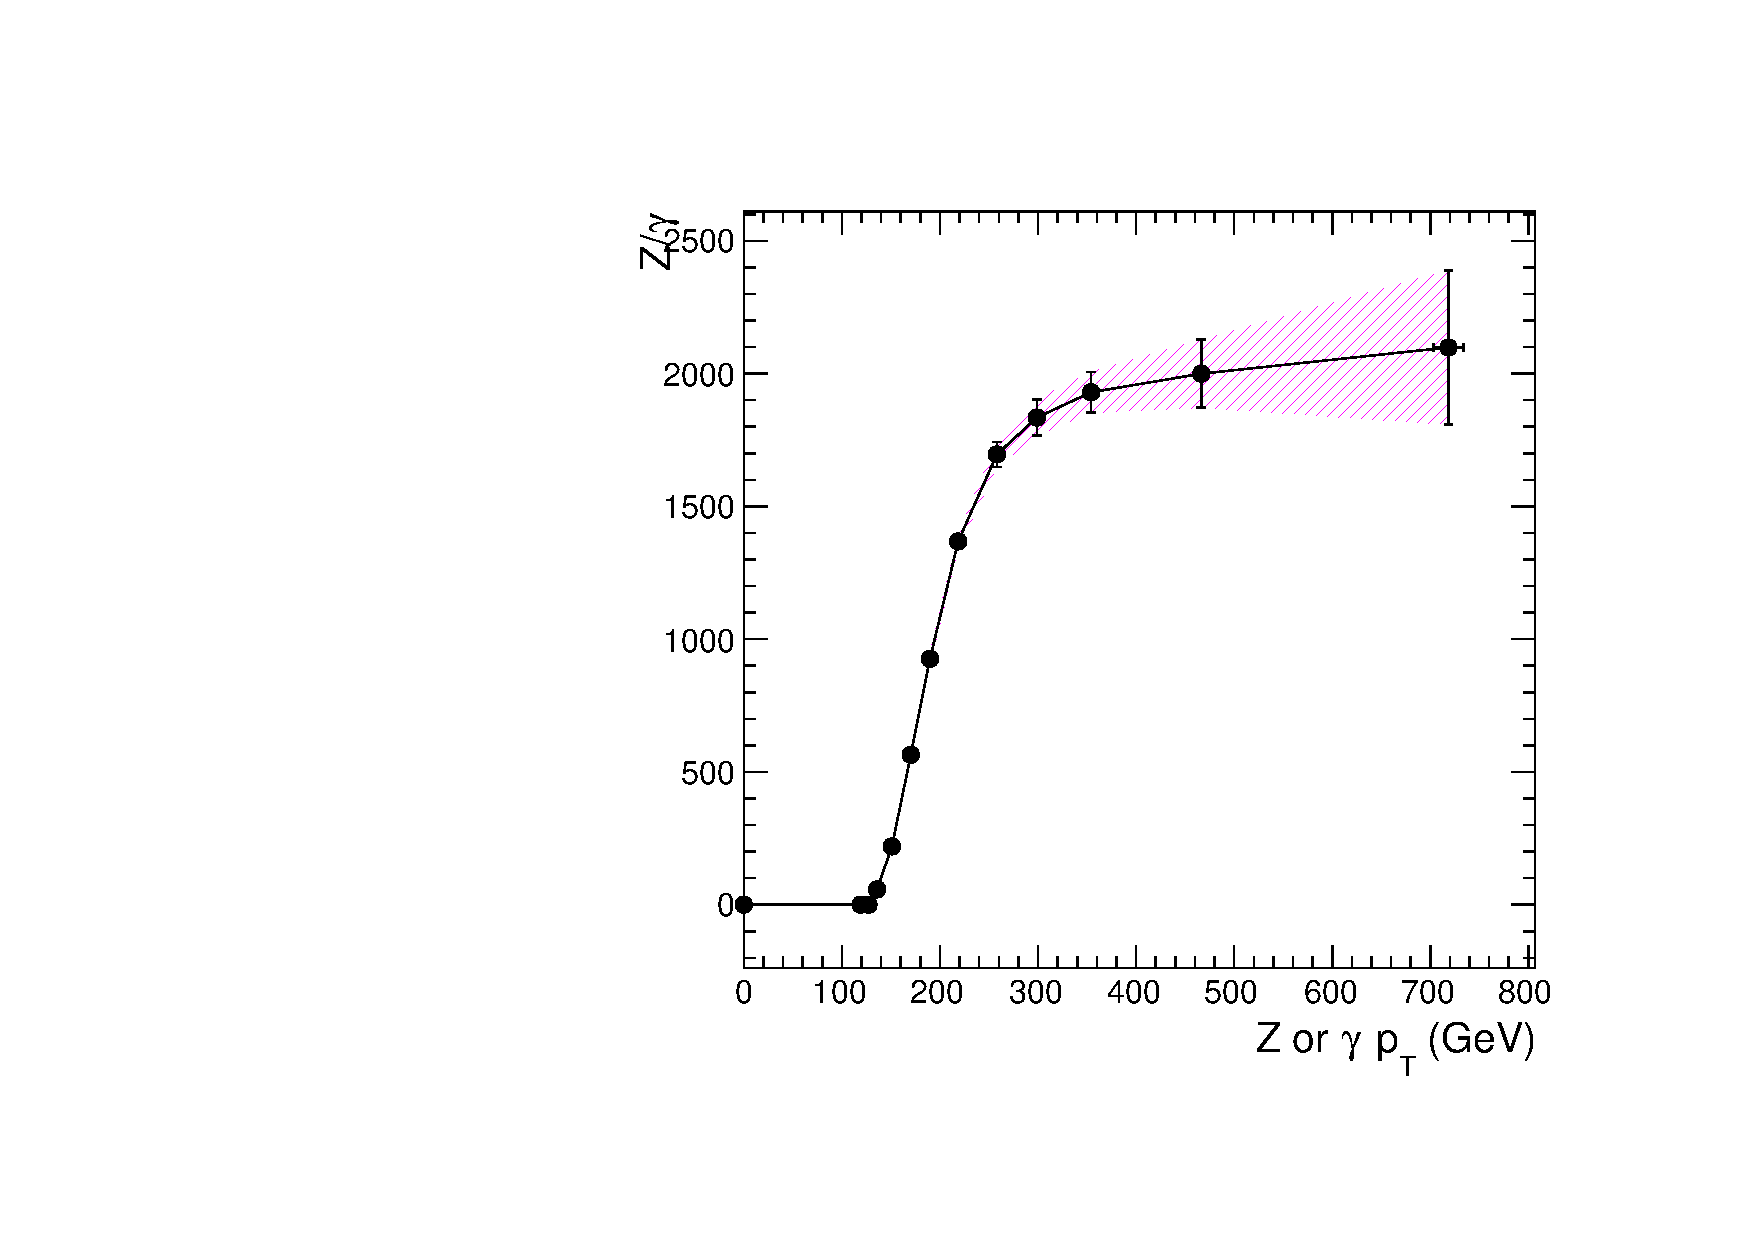
\includegraphics[width=0.9\linewidth]{figures/study_gjets_data_allcorV2_modify_el.pdf}
  \caption{Photon $p_T$ reweighting function for the electron channel.
 The uncertainty bands includes uncertainties from 2015 CMS \Zjets differential cross-section measurements, the statistical uncertainty from \Zjets MC sample and \gjets data sample, and the lepton trigger, ID, ISO efficiency scale factors.}
  \label{fig:photon_pt_weight_el}
\end{figure}

\begin{figure}[htbp]
\centering
  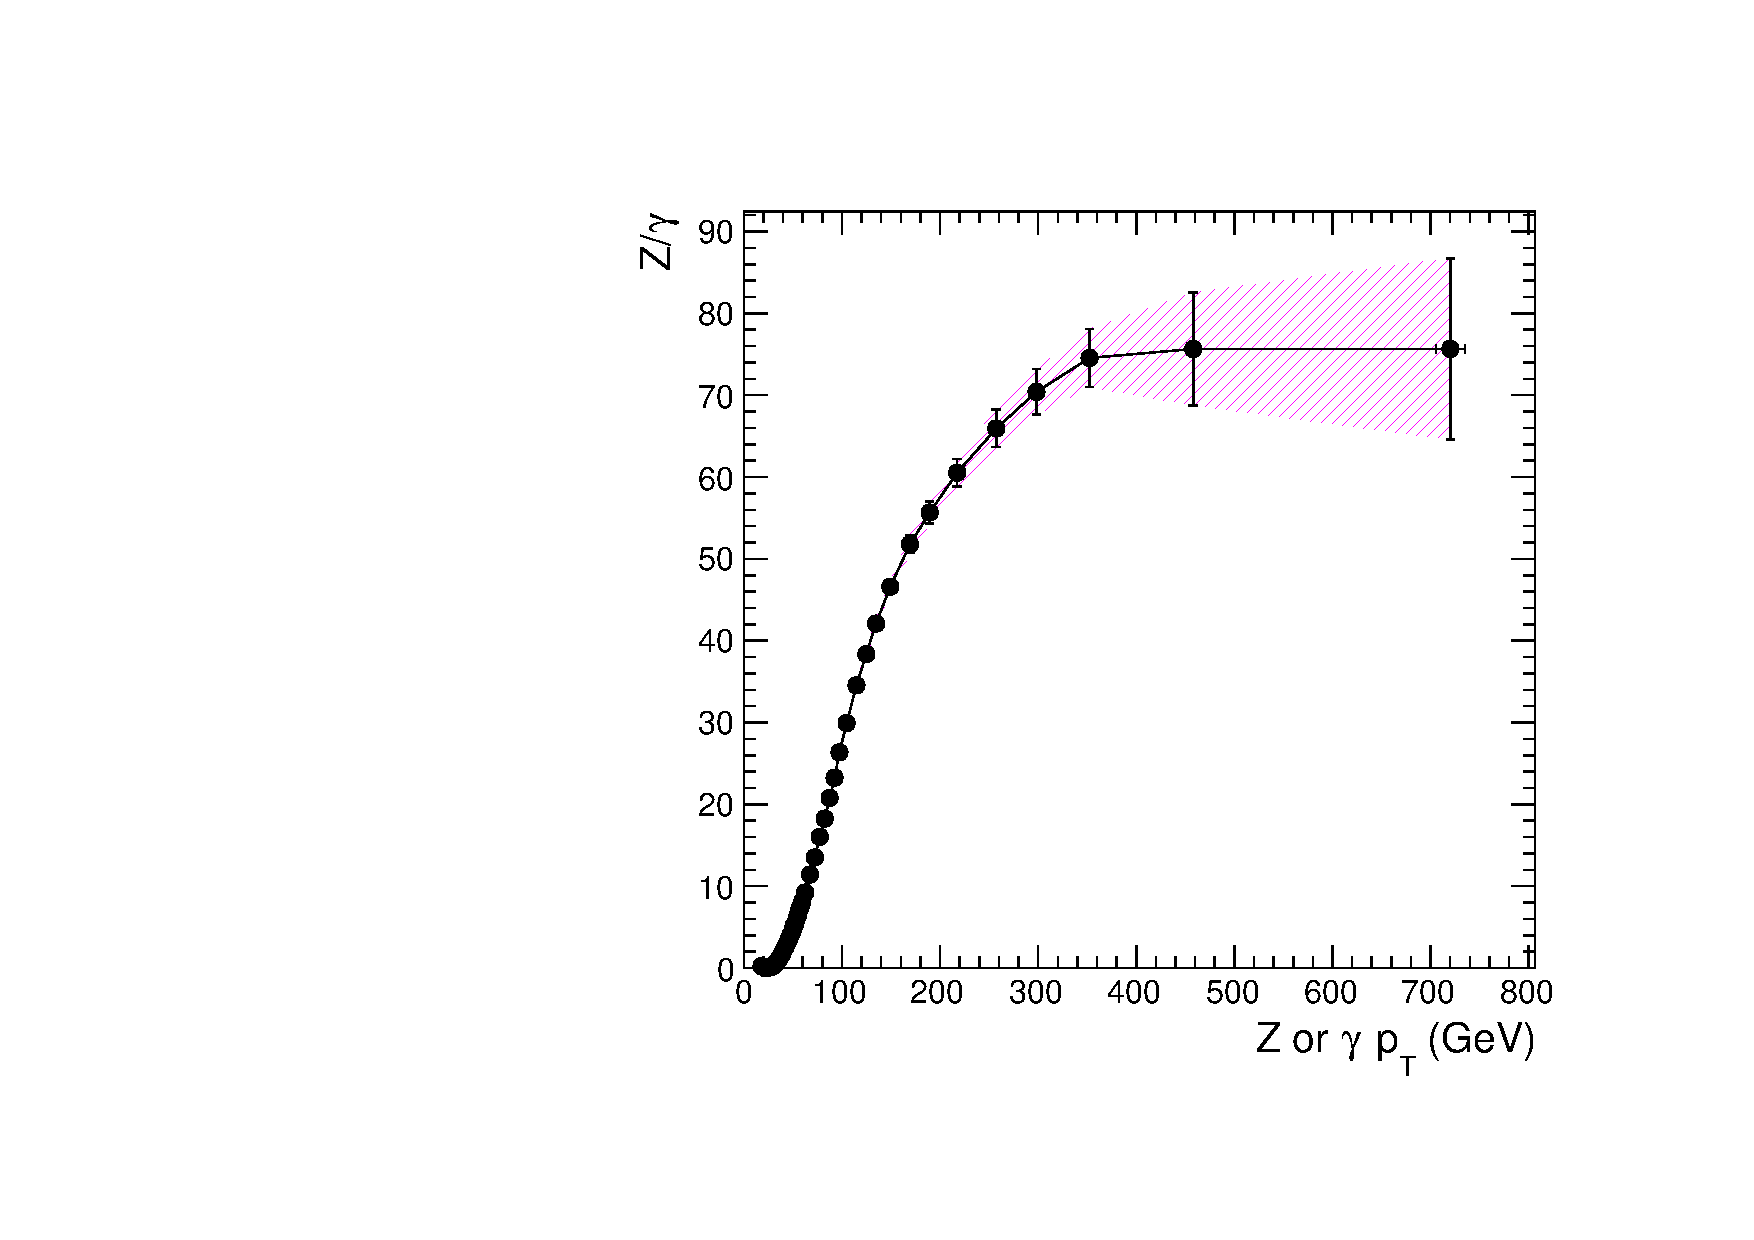
\includegraphics[width=0.9\linewidth]{figures/study_gjets_data_allcorV2_modify_mu.pdf}
  \caption{Photon $p_T$ reweighting function for the muon channel.
 The uncertainty bands includes uncertainties from 2015 CMS \Zjets differential cross-section measurements, the statistical uncertainty from \Zjets MC sample and \gjets data sample, and the lepton trigger, ID, ISO efficiency scale factors.}
  \label{fig:photon_pt_weight_mu}
\end{figure}

\subsection{Photon Mass Generation}\label{sec:gjetm}
The mass of the leptonic Z boson is used in the transverse mass calculation (Equation~\ref{eqn:intro_MT}, \ref{eqn:intro_MTalt}), and must be simulated in the \gjets events to model the $m_T$ in the \Zjets background. This is done by assigning a random mass to the photon based on the Z boson mass distribution and parameterized as a function of Z boson $p_T$.

\vspace{0.3cm}
Figures~\ref{fig:mz_el_zjets_gjets} and \ref{fig:mz_mu_zjets_gjets}, compare the Z mass distributions of \Zjets MC and the simulated Z mass for \gjets data events, for electron and muon channels separately.

\begin{figure}[htbp!]
\centering
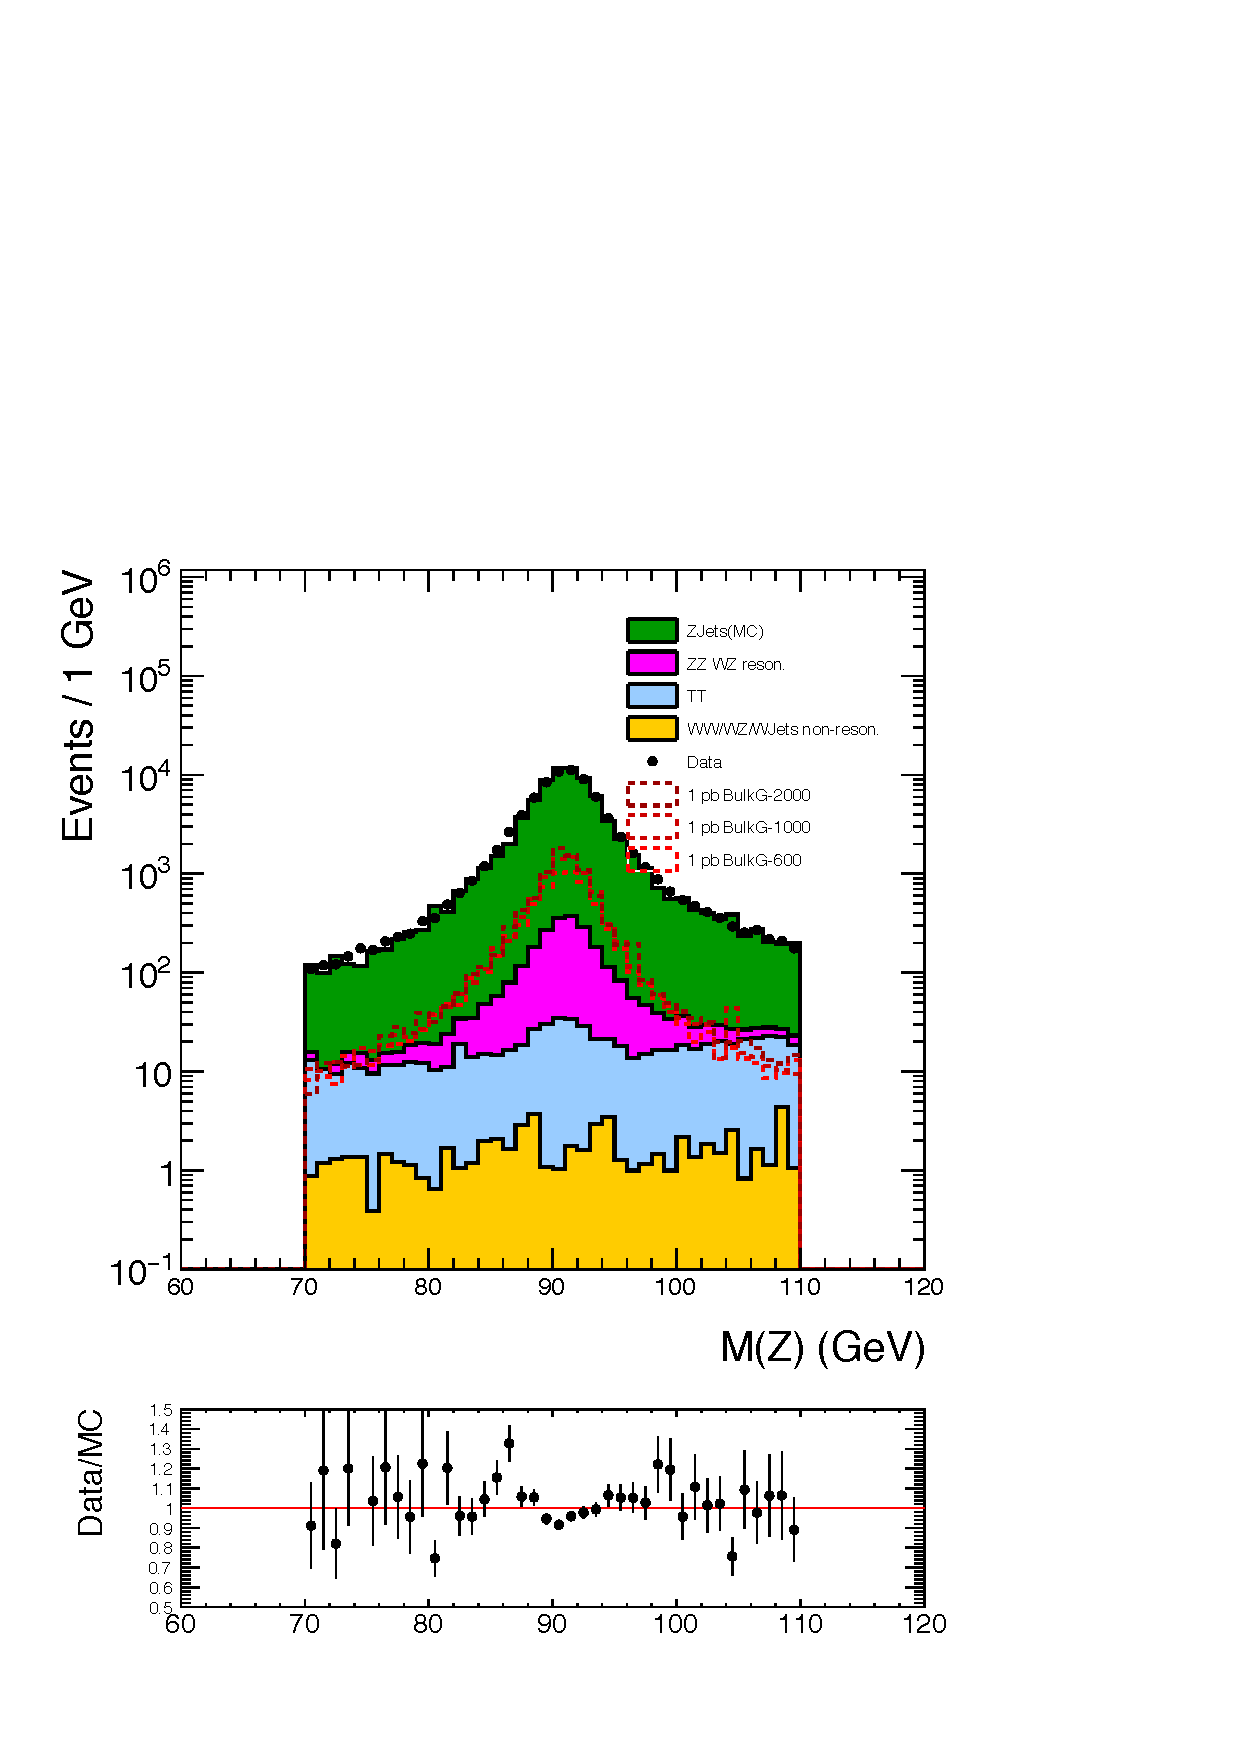
\includegraphics[width=0.46\linewidth]{figures/MC2_Rc36p46DtReCalib_RhoWt_GMCEtaWt_tightzpt50_puWeightmoriondMC_metfilter_el_log_1pb.pdf}
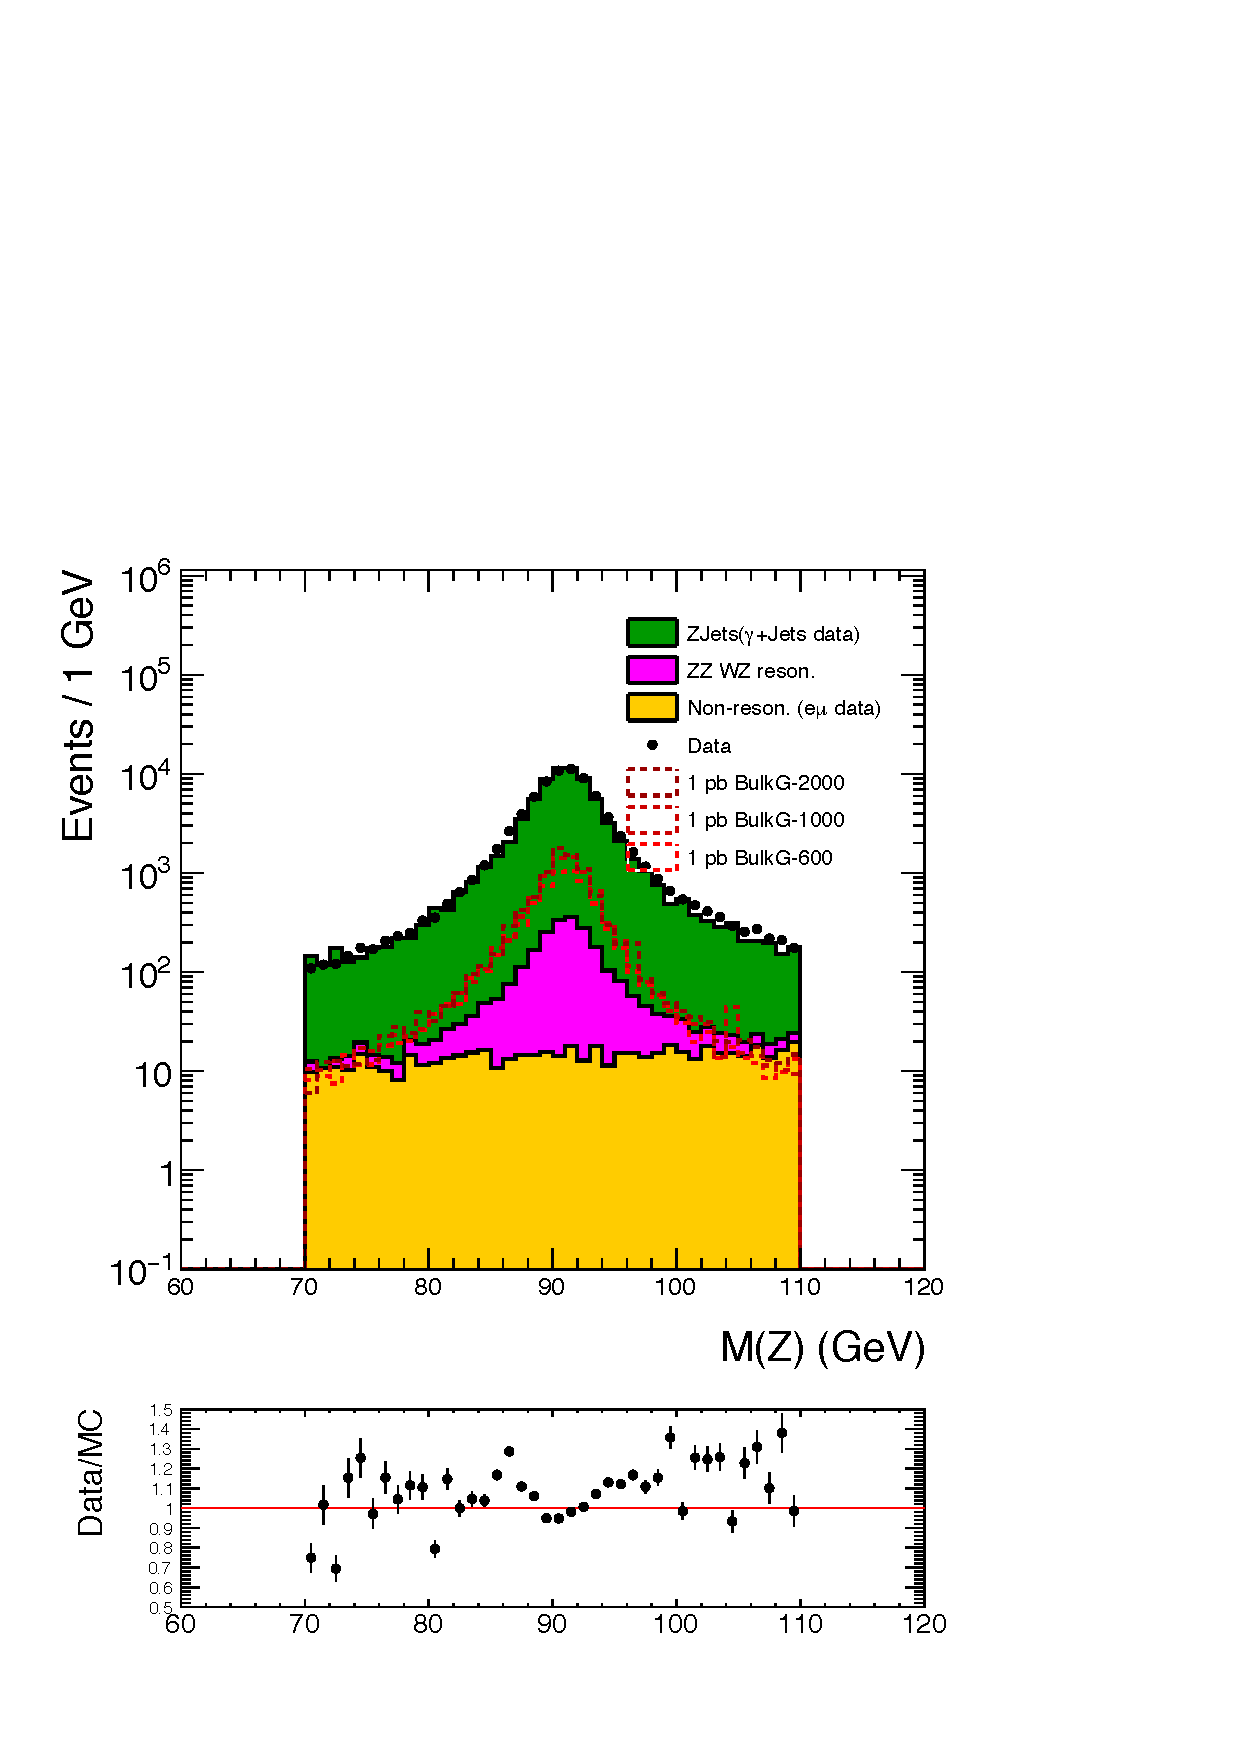
\includegraphics[width=0.46\linewidth]{figures/GJets2_BkgSub_Rc36p46DtReCalib_NonReso_RhoWt_GMCEtaWt_tightzpt50_puWeightmoriondMC_muoneg_gjet_metfilter_el_log_1pb.pdf}
\caption{Z mass distributions for electron channel, comparing \Zjets MC (left) and the simulated Z mass for \gjets data events (right).}
\label{fig:mz_el_zjets_gjets}
\end{figure}

\begin{figure}[htbp!]
\centering
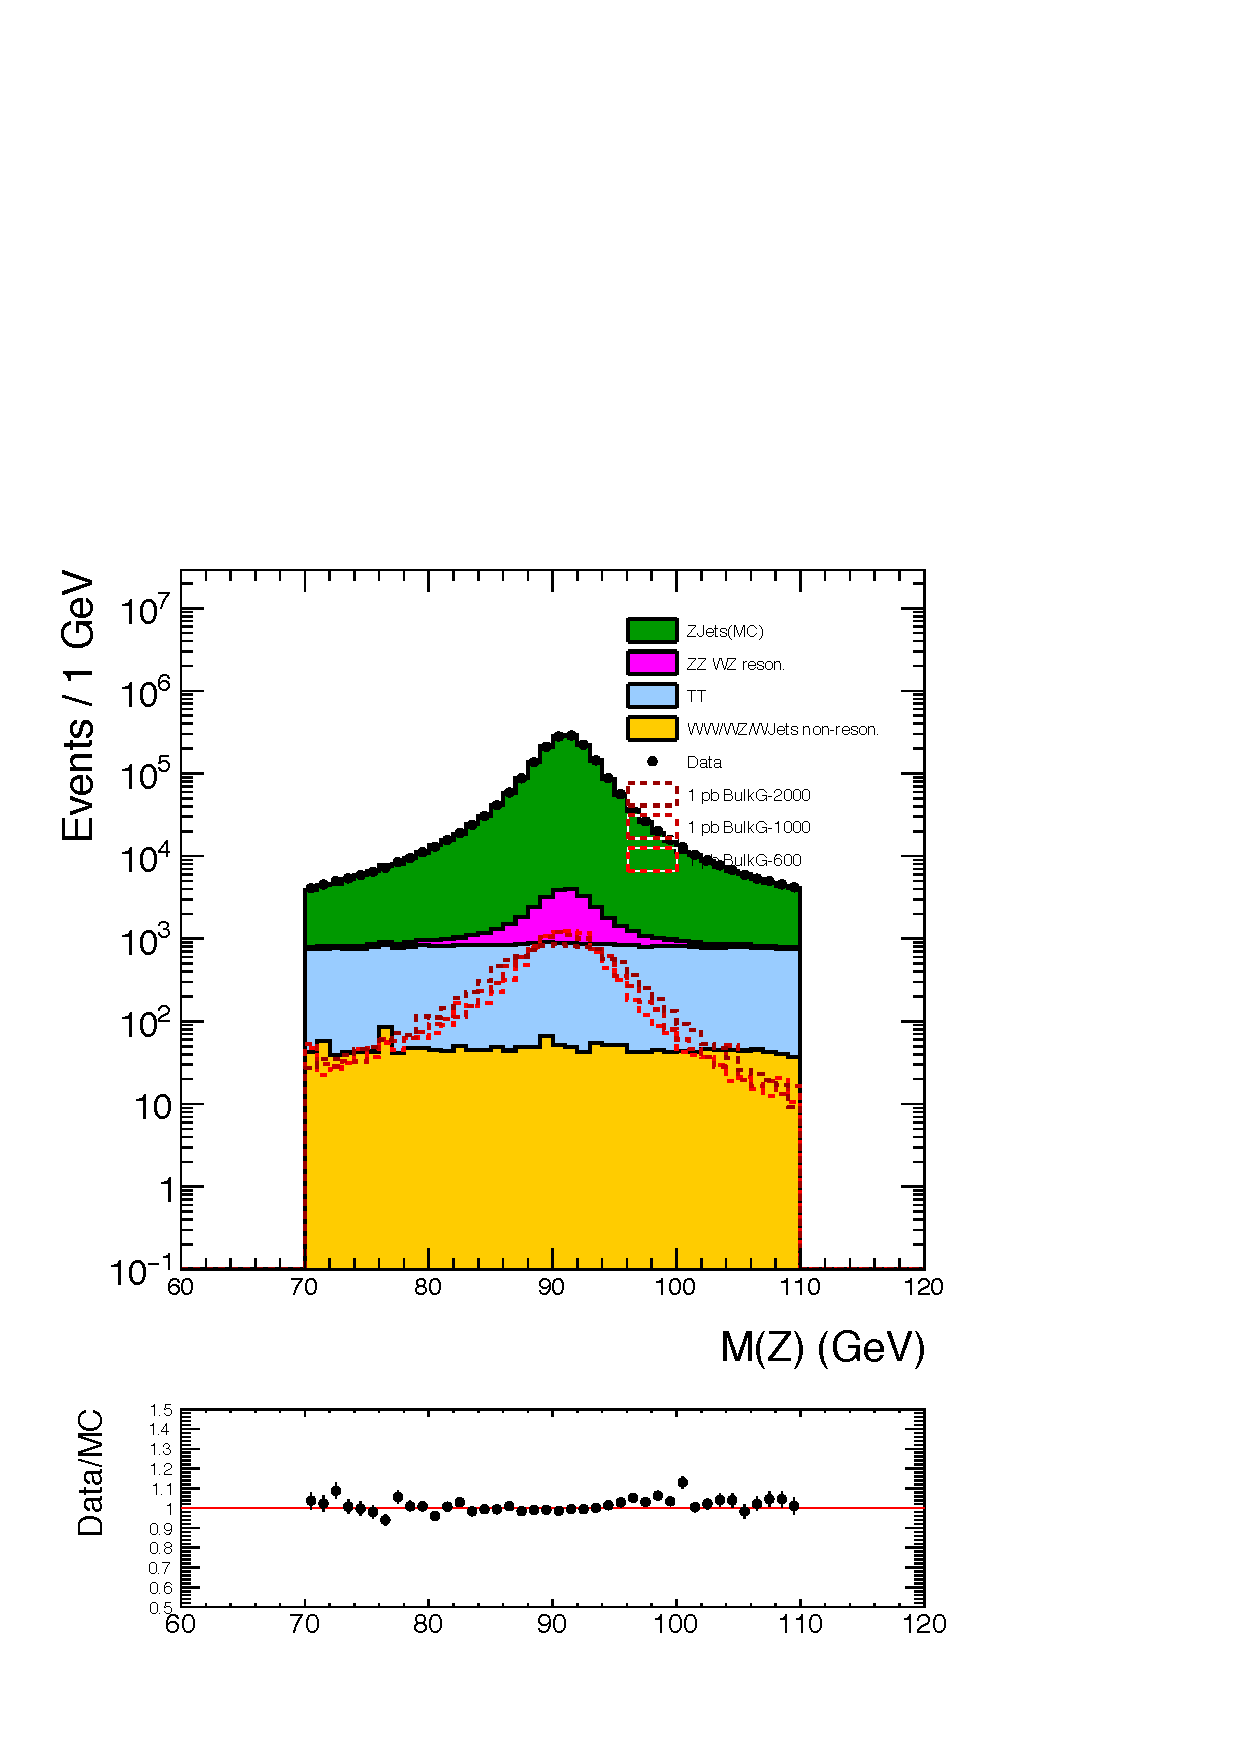
\includegraphics[width=0.46\linewidth]{figures/MC2_Rc36p46DtReCalib_RhoWt_GMCEtaWt_tightzpt50_puWeightmoriondMC_metfilter_mu_log_1pb.pdf}
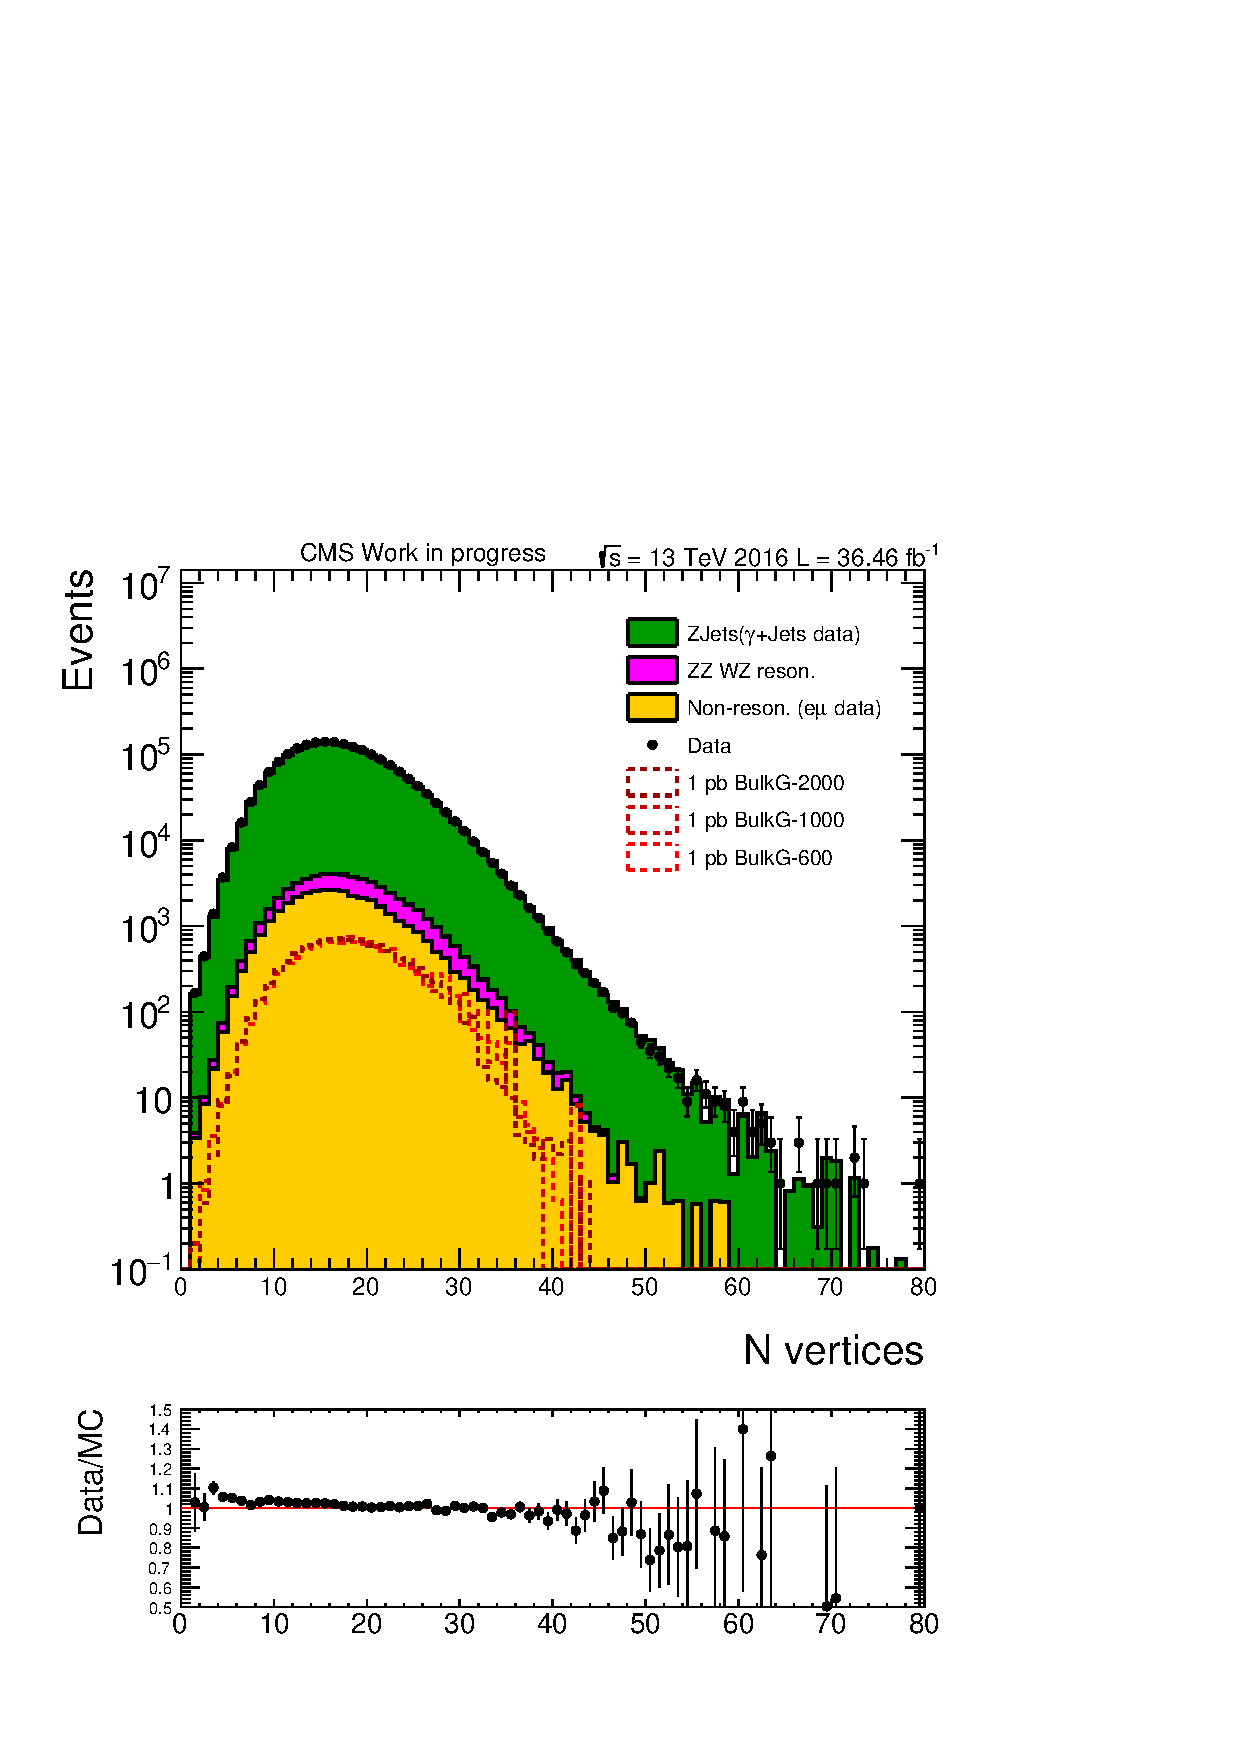
\includegraphics[width=0.46\linewidth]{figures/GJets2_BkgSub_Rc36p46DtReCalib_NonReso_RhoWt_GMCEtaWt_tightzpt50_puWeightmoriondMC_muoneg_gjet_metfilter_mu_log_1pb.pdf}
\caption{Z mass distributions for muon channel, comparing \Zjets MC (left) and the simulated Z mass for \gjets data events (right).}
\label{fig:mz_mu_zjets_gjets}
\end{figure}

\subsection{\boldmath{\ptmiss} Hadronic Recoil Tuning}\label{sec:gjetmet}
The \Zjets process consists of a Z boson decaying to a lepton pair and a hadronic recoil balancing the Z boson $p_T$ in the transverse plain. As a result, in theory the \ptmiss should be 0. However, due to limitations of the detector resolutions for leptons and jets, \ptmiss is present in \Zjets process due to instrumental effects. The energy resolution of leptons, jets, photons are potentially different between \gjets data and \Zjets data, and those differences may introduce differences in the resolution and scale of reconstructed \ptmiss.

\vspace{0.3cm}
A single-Gaussian based hadronic recoil fit is developed to tune the \ptmiss of the \gjets data to match the \ptmiss in the \Zjets data. The general idea is to apply a correction to the \gjets data to better discribe the ${p_{T}}^{miss}_\parallel$ and ${p_{T}}^{miss}_\perp$ distributions of the \Zjets process, where ${p_{T}}^{miss}_\parallel$ refers to the projection of \ptmiss in the direction of ${p}_{T}^{z(\gamma)}$ and ${p_{T}}^{miss}_\perp$ is the fraction perpendicular to ${p}_{T}^{z(\gamma)}$. 

\vspace{0.3cm}
The ${p_{T}}^{miss}_\parallel$ and ${p_{T}}^{miss}_\perp$ are fit with a Gaussian function in the region of [-50, 50]\GeV. The Gaussian mean values and resolutions are parameterized as functions of the $p_T$ of Z boson and photon. Figure~\ref{fig:recoilfit_example_data} gives some example plots showing the Gaussian fits for the $p_T$ bins 50-60\GeV for \Zjets data, for muon channel and electron channel, for ${p_{T}}^{miss}_\parallel$ and ${p_{T}}^{miss}_\perp$, respectively.
\begin{figure}[htbp]
\begin{center}
\includegraphics[width=0.46\linewidth, page=21]{figures/SingleEMU_Run2016Full_03Feb2017_allcorV2_met_para_study_ZSelecLowLPt_mu.pdf}
\includegraphics[width=0.46\linewidth, page=56]{figures/SingleEMU_Run2016Full_03Feb2017_allcorV2_met_para_study_ZSelecLowLPt_mu.pdf}
\includegraphics[width=0.46\linewidth, page=21]{figures/SingleEMU_Run2016Full_03Feb2017_allcorV2_met_para_study_ZSelecLowLPt_el.pdf}
\includegraphics[width=0.46\linewidth, page=56]{figures/SingleEMU_Run2016Full_03Feb2017_allcorV2_met_para_study_ZSelecLowLPt_el.pdf}
\caption{Example plots for the single Gaussian-based \ptmiss hadronic recoil fit of a selected Z $p_T$ bin for \Zjets data, muon channel (upper), electron channel (lower), ${p_{T}}^{miss}_\parallel$ (left), ${p_{T}}^{miss}_\perp$ (right).}
\label{fig:recoilfit_example_data}
\end{center}
\end{figure}


\vspace{0.3cm}
The comparison of the recoil fit results between \Zjets data and \gjets data before correction are shown in 
Figures~\ref{fig:recoilfit_met_peak_reso_compare_data_gjets_mu}
and \ref{fig:recoilfit_met_peak_reso_compare_data_gjets_el}
for muon channel and electron channel, respectively. 

\begin{figure}[htbp]
\begin{center}
\includegraphics[width=0.46\linewidth, page=1]{figures/plots_SingleEMU_Run2016Full_03Feb2017_allcorV2_met_para_study_ZSelecLowLPt_mu_VS_SinglePhoton_Run2016Full_03Feb2017_allcorV2_NoRecoil_met_para_study_ZSelecLowLPt_mu.pdf}
\includegraphics[width=0.46\linewidth, page=5]{figures/plots_SingleEMU_Run2016Full_03Feb2017_allcorV2_met_para_study_ZSelecLowLPt_mu_VS_SinglePhoton_Run2016Full_03Feb2017_allcorV2_NoRecoil_met_para_study_ZSelecLowLPt_mu.pdf}
\includegraphics[width=0.46\linewidth, page=3]{figures/plots_SingleEMU_Run2016Full_03Feb2017_allcorV2_met_para_study_ZSelecLowLPt_mu_VS_SinglePhoton_Run2016Full_03Feb2017_allcorV2_NoRecoil_met_para_study_ZSelecLowLPt_mu.pdf}
\includegraphics[width=0.46\linewidth, page=7]{figures/plots_SingleEMU_Run2016Full_03Feb2017_allcorV2_met_para_study_ZSelecLowLPt_mu_VS_SinglePhoton_Run2016Full_03Feb2017_allcorV2_NoRecoil_met_para_study_ZSelecLowLPt_mu.pdf}
\caption{Comparison of the recoil fitted peak positions and Gaussian resolutions for ${p_{T}}^{miss}_\parallel$ and ${p_{T}}^{miss}_\perp$ between di-lepton data and \gjets data for the muon channel. Upper two for 
${p_{T}}^{miss}_\parallel$, bottom two for ${p_{T}}^{miss}_\perp$.}
\label{fig:recoilfit_met_peak_reso_compare_data_gjets_mu}
\end{center}
\end{figure}

\begin{figure}[htbp]
\begin{center}
\includegraphics[width=0.46\linewidth, page=1]{figures/plots_SingleEMU_Run2016Full_03Feb2017_allcorV2_met_para_study_ZSelecLowLPt_el_VS_SinglePhoton_Run2016Full_03Feb2017_allcorV2_NoRecoil_met_para_study_ZSelecLowLPt_el.pdf}
\includegraphics[width=0.46\linewidth, page=5]{figures/plots_SingleEMU_Run2016Full_03Feb2017_allcorV2_met_para_study_ZSelecLowLPt_el_VS_SinglePhoton_Run2016Full_03Feb2017_allcorV2_NoRecoil_met_para_study_ZSelecLowLPt_el.pdf}
\includegraphics[width=0.46\linewidth, page=3]{figures/plots_SingleEMU_Run2016Full_03Feb2017_allcorV2_met_para_study_ZSelecLowLPt_el_VS_SinglePhoton_Run2016Full_03Feb2017_allcorV2_NoRecoil_met_para_study_ZSelecLowLPt_el.pdf}
\includegraphics[width=0.46\linewidth, page=7]{figures/plots_SingleEMU_Run2016Full_03Feb2017_allcorV2_met_para_study_ZSelecLowLPt_el_VS_SinglePhoton_Run2016Full_03Feb2017_allcorV2_NoRecoil_met_para_study_ZSelecLowLPt_el.pdf}
\caption{Comparison of the recoil fitted peak positions and Gaussian resolutions for ${p_{T}}^{miss}_\parallel$ and ${p_{T}}^{miss}_\perp$ between di-lepton data and \gjets data for the electron channel. Upper two for 
${p_{T}}^{miss}_\parallel$, bottom two for ${p_{T}}^{miss}_\perp$.}
\label{fig:recoilfit_met_peak_reso_compare_data_gjets_el}
\end{center}
\end{figure}

The \gjets data ${p_{T}}^{miss}_\parallel$ peak and the resolution of ${p_{T}}^{miss}_\parallel$ and ${p_{T}}^{miss}_\perp$ are then corrected to match the \Zjets data respectively for muon and electron channels based on Figures~\ref{fig:recoilfit_met_peak_reso_compare_data_gjets_mu} and \ref{fig:recoilfit_met_peak_reso_compare_data_gjets_el}. The correction for the photon data is done in the following way:
\begin{itemize}
\item Shift the ${p_{T}}^{miss}_\parallel$ peak positions of \gjets data to match that of the \Zjets data;
\item Scale the ${p_{T}}^{miss}_\parallel$ and ${p_{T}}^{miss}_\perp$ resolution of \gjets data to match that of the \Zjets data.
\end{itemize}

The peak position correction is only applied to ${p_{T}}^{miss}_\parallel$, as the \ptmiss results from the instrumental imbalance between the Z boson and hadronic recoil, therefore the distribution of ${p_{T}}^{miss}_\parallel$ is more imbalanced while the peak position for ${p_{T}}^{miss}_\perp$ is expected to be 0.

\clearpage
\section{Non-resonant Background Modeling}
The non-resonant background contains mostly $t\bar{t}$ and WW events. A data driven method is used in the analysis to model the non-resonant background. The method is to use the $e\mu$ pairs to describe the non-resonant background in $\ell\ell$ ($ee$ or $\mu \mu$) events, based on the fact that in $t\bar{t}$ and WW decays, $e\mu$ pairs have similar kinematic behavior and cross-section as the $\ell\ell$ ($ee$ or $\mu \mu$) decay states.

\subsection{\boldmath{$e\mu$} Pair Selection}
The 35.8 fb$^{-1}$ 2016 MuonEG dataset is used for the $e\mu$ pair selection.  Events with one or more $e\mu$ pair are selected. If more than one $e\mu$ pair is present in an event, the pair with invariant mass closest to Z boson mass is selected (analogous to the data selection). Electrons are required to pass Loose ID with pfIso, and muons are required to pass High $p_T$ ID and tracker isolation. 

\vspace{0.3cm}
When the $e\mu$ sample is used as background in the electron channel the selections below are applied to match the requirements applied in data: 
\begin{itemize}
\item Leading lepton $p_{T}>120\GeV$, $|\eta|<2.5$, 
\item Subleading lepton $p_{T}>35\GeV$, $|\eta|<2.5$
\end{itemize}
When the sample is used in the muon channel the selections are:
\begin{itemize}
\item Leading lepton $p_{T}>55\GeV$, $|\eta|<2.4$
\item Subleading lepton $p_{T}>20\GeV$, $|\eta|<2.4$. 
\end{itemize}

\subsection{\boldmath{$e\mu$} Pair Event-based Reweighting}
Based on the assumption that electrons and muons have the same behavior in the non-resonant background, the distributions of kinematic variables for the electron and muon in the $e\mu$ pair are expected to be nearly identical. However, this symmetry is altered by triggers and reconstruction effects. Figure~\ref{fig:nonresmuelpt} shows the $p_T$ distribution of the electrons and muons, and their ratio in the MuonEG dataset.

\begin{figure}[htbp]
\begin{center}
\includegraphics[width=0.95\linewidth]{figures/nonresmuelpt.png}
\caption{electron and muon $p_T$ distribution (left) and ratio (right) in the $e\mu$ pair sample selected from MuonEG dataset.}
\label{fig:nonresmuelpt}
\end{center}
\end{figure}

\vspace{0.3cm}
The discrepancy between the $p_T$ distributions of electrons and muons can result from many factors, such as detector effects, triggers, identification criteria and isolation efficiencies. Event based weighting factors are calculated according to the ratio plot in Figure~\ref{fig:nonresmuelpt}(right). When modeling the electron channel, the correction factor of the event is set to be the ratio value corresponding to the muon $p_T$ in the $e\mu$ event. Conversly, when modeling the muon channel, the correction factor of the event is the inverse of the ratio value corresponding to the electron $p_T$.

\vspace{0.3cm}
Figure~\ref{fig:nonresmuelptel} shows the electron and muon $p_T$ distribution and ratio after the correction for the electron channel, and Figure~\ref{fig:nonresmuelptmu} is for the muon channel.

\begin{figure}[htbp]
\begin{center}
\includegraphics[width=0.95\linewidth]{figures/nonresmuelptel.png}
\caption{electron and muon $p_T$ distribution (left) and ratio (right) in the $e\mu$ pair sample (from MuonEG dataset) after the event based reweighting for the electron channel}
\label{fig:nonresmuelptel}
\end{center}
\end{figure}

\begin{figure}[htbp]
\begin{center}
\includegraphics[width=0.95\linewidth]{figures/nonresmuelptmu.png}
\caption{electron and muon $p_T$ distribution (left) and ratio (right) in the $e\mu$ pair sample (from MuonEG dataset) after the event based reweighting for the muon channel}
\label{fig:nonresmuelptmu}
\end{center}
\end{figure}

\vspace{0.3cm}
The agreement between the $p_T$ distributions of electrons and muons are improved with the event based reweighting for both the electron channel and muon channel. In the electron channel, both leptons behave like the electron before weighting, and in the muon channel both leptons behave like the muon before weighting. This reweighting suppresses the systematic uncertainty caused by the performance discrepancy between electrons and muons due to detector and reconstruction effects. With the reweighting there is still a ~2\% of disagreement between the $p_T$ distributions of electrons and muons, and this is quoted as the systematic uncertainty of the method.

\subsection{HLT Efficiency Reweighting}
The effect of the HLT in our $\ell \ell$ data selection is calculated and applied in the $e\mu$ sample to simulate the single lepton HLT. With the event based reweighting described above, the electrons and muons in the $e\mu$ pair sample behave very similarly and can be treated as $\ell \ell$ pairs for the purpose of background studies. Both SingleElectron and SingleMuon trigger efficiency for data are calculated for each event in the $e\mu$ pair data, corresponding to the leading lepton's $p_T$ and $\eta$, regardless of whether the leading lepton is a muon or an electron. The trigger efficiency for data is described in Section~\ref{sec:bkg_trig}. The SingleElectron trigger efficiency is applied when the sample is used in the electron channel, similarly the SingleMuon trigger efficiency is applied when the sample is used in the muon channel. The uncertainty of the trigger efficiency is evaluated and quoted as the standard deviation of the efficiencies among all the selected events for each channel (see Table~\ref{tab:nonresuncert}).

\vspace{0.3cm}
When applying the SingleLepton trigger efficiency on the MuonEG dataset to emulate the data HLT, the MuonEG dataset is expected to have full acceptance in our preselection region. This explains why no HLT is required in the MuonEG data selection process. By not requiring any MuonEG HLT, events passing any MuonEG HLTs are accepted. Considering the high $p_T$ threshold in the lepton selection, the acceptance of the dataset is high enough and this effect can be ignored compared to the single lepton trigger efficiency uncertainty. In fact, the acceptance of the MuonEG dataset has negligible effect as long as it is consistent in our preselection region, and the $e\mu$ sample is rescaled as discussed below. To clarify, the $p_T$ thresholds of the MuonEG dataset do not affect our event selection. For the muon channel, we require a leading lepton $pt>60\GeV$, and subleading lepton $pt>20\GeV$. The electron channel has higher lepton $p_T$ selection. The MuonEG dataset contains non-prescaled triggers:
\begin{itemize}
\item \texttt{HLT\_Mu23\_TrkIsoVVL\_Ele12\_CaloIdL\_TrackIdL\_IsoVL(\_DZ)} 
\item \texttt{HLT\_Mu12\_TrkIsoVVL\_Ele23\_CaloIdL\_TrackIdL\_IsoVL(\_DZ)}
\end{itemize}
and these $p_T$ thresholds are much lower than our $p_T$ selection.

\subsection{\boldmath{$e\mu$} Events Rescaling}
The selected $e\mu$ sample must be scaled to estimate the background in the selected data. To rescale the $e\mu$ samples to fit the non-resonant background and study the agreement of the background sample and data, a non-resonant control region is defined. The scale factor is calculated by equation~\ref{eq:nonresscale}.
\begin{equation} \label{eq:nonresscale}
  Scale  =  \frac{N_{data,ll}-N_{MC,reson}}{N_{data,e\mu}}
\end{equation}

The $N_{data,ll}$ is the number of data events in the control region; $N_{MC,reson}$ is the number of background Z events in the control region, including \Zjets background and resonant background; the $N_{data,e\mu}$ is the number of $e\mu$ pair events in the control region. To define the control region, the main idea is to suppress the standard deviation of the calculated scale factor. The standard deviation is calculated based on equation~\ref{eq:nonresscale}, and given in equation~\ref{eq:nonresscaledev}.
\begin{equation} \label{eq:nonresscaledev}
  \sigma_{Scale}  = \sqrt{\frac{\sigma^{2}_{N_{data,ll}}+\sigma^{2}_{N_{MC,reson}}}{(N_{data,ll}-N_{MC,reson})^{2}}+\frac{\sigma^{2}_{N_{data,e\mu}}}{N^{2}_{data,e\mu}}}\times \frac{N_{data,ll}-N_{MC,reson}}{N_{data,e\mu}}
\end{equation}

Here the statistical uncertainty is considered for both MC and data, and the PDF uncertainty is considered for resonant MC (1.5\%).

\vspace{0.3cm}
To suppress scale deviation and resonant background in the CR, selections below are applied: 
\begin{enumerate}
\item Z mass veto: invariant mass $M<70\GeV$ or $M>110\GeV$; 
\item $p_{T}^{Z} > X\GeV$;
\end{enumerate}

To determine the X value ($p_{T}^{Z}$ cut level), a scan over various X values is performed. The calculated scale factor and uncertainty vs X is shown in Table~\ref{tab:nonressfdev}. X=60 gives relatively small uncertainty, and is used to define the control region. The scale uncertainty corresponding to X=60 is also counted as the systematic uncertainty.

\begin{table}[htbp]
  \begin{center}
    \caption{
      scale and deviation vs X($p_{T}^{Z}$ cut value) scan result.      
      \label{tab:nonressfdev}}
    \begin{tabular}{c c c}
      \hline\hline
      X & electron channel scale & muon channel scale\\
      \hline
      0  & 0.3442$\pm$0.0140 & 0.8215$\pm$0.0519 \\
      10 & 0.3442$\pm$0.0140 & 0.7762$\pm$0.0388 \\
      20 & 0.3442$\pm$0.0140 & 0.7364$\pm$0.0290 \\
      30 & 0.3442$\pm$0.0140 & 0.7046$\pm$0.0238 \\
      40 & 0.3442$\pm$0.0140 & 0.6962$\pm$0.0202 \\
      50 & 0.3443$\pm$0.0140 & 0.6895$\pm$0.0182 \\
      60 & 0.3463$\pm$0.0140 & 0.6871$\pm$0.0171 \\
      70 & 0.3490$\pm$0.0142 & 0.6907$\pm$0.0167 \\
      80 & 0.3560$\pm$0.0146 & 0.6952$\pm$0.0170 \\
      90 & 0.3635$\pm$0.0156 & 0.7092$\pm$0.0182 \\
      100 & 0.3733$\pm$0.0169 & 0.7249$\pm$0.0205 \\
      110 & 0.3771$\pm$0.0186 & 0.7402$\pm$0.0234 \\
      \hline\hline
    \end{tabular}
  \end{center}
\end{table}

\vspace{0.3cm}
Electron channel plots in the control region are shown in Figure~\ref{fig:nonreselcr} and those for the muon channel are shown in the Figure~\ref{fig:nonresmucr}.

\begin{figure}[htbp]
\begin{center}
\includegraphics[width=0.39\linewidth, page=1]{figures/test_metzpt50_RhoWt_puWeight68075_metfilter_el_.pdf}
\includegraphics[width=0.39\linewidth, page=2]{figures/test_metzpt50_RhoWt_puWeight68075_metfilter_el_.pdf}
\includegraphics[width=0.39\linewidth, page=3]{figures/test_metzpt50_RhoWt_puWeight68075_metfilter_el_.pdf}
\includegraphics[width=0.39\linewidth, page=4]{figures/test_metzpt50_RhoWt_puWeight68075_metfilter_el_.pdf}
\caption{Data-driven non-resonant background in the control region, electron channel plots}
\label{fig:nonreselcr}
\end{center}
\end{figure}

\begin{figure}[htbp]
\begin{center}
\includegraphics[width=0.39\linewidth, page=1]{figures/test_metzpt50_RhoWt_puWeight68075_metfilter_mu_.pdf}
\includegraphics[width=0.39\linewidth, page=2]{figures/test_metzpt50_RhoWt_puWeight68075_metfilter_mu_.pdf}
\includegraphics[width=0.39\linewidth, page=3]{figures/test_metzpt50_RhoWt_puWeight68075_metfilter_mu_.pdf}
\includegraphics[width=0.39\linewidth, page=4]{figures/test_metzpt50_RhoWt_puWeight68075_metfilter_mu_.pdf}
\caption{Data-driven non-resonant background in the control region, muon channel plots}
\label{fig:nonresmucr}
\end{center}
\end{figure}

\vspace{0.3cm}
The control region plots show that the resonant background is heavily suppressed in the CR and data driven non-resonant background agrees well with the data. Also non-resonant $e\mu$ events should have similar cross section compared to those in $\ell\ell$ events, which means that the sum of the scale factors in the electron channel and the muon channel should be close to 1. From Table~\ref{tab:nonressfdev} we see that at X=60, the scale factor is 0.346 for the electron channel, and 0.687 for the muon channel, adding up to 1.033, which agrees with the prediction.

\subsection{Comparing to MC Modeling}
Figure~\ref{fig:nonreselzmasscr100} is a comparison of the non-resonant background modeled by the data-driven method and the $t\bar{t}+WW$ MC samples as a cross-check of the data-driven method, with $70\GeV<M_{Z}<110\GeV$, $\ptmiss >50\GeV$ and $p_{T}^{Z}>100\GeV$ (standard signal region selections in this analysis), for electron channel. Similarly Figure~\ref{fig:nonresmuzmasscr100} shows the result for the muon channel. The data-driven modeling method generally gives a very similar non-resonant background distribution as the MC. However, in the electron channel the yield of the data-driven method is slightly higher than the MC modeling.

\begin{figure}[htbp]
\begin{center}
\includegraphics[width=0.39\linewidth, page=1]{figures/test_zpt100_log_RhoWt_puWeight68075_metfilter_el_.pdf}
\includegraphics[width=0.39\linewidth, page=3]{figures/test_zpt100_log_RhoWt_puWeight68075_metfilter_el_.pdf}
\includegraphics[width=0.39\linewidth, page=6]{figures/test_zpt100_log_RhoWt_puWeight68075_metfilter_el_.pdf}
\includegraphics[width=0.39\linewidth, page=2]{figures/test_zpt100_log_RhoWt_puWeight68075_metfilter_el_.pdf}
\includegraphics[width=0.39\linewidth, page=5]{figures/test_zpt100_log_RhoWt_puWeight68075_metfilter_el_.pdf}
\includegraphics[width=0.39\linewidth, page=4]{figures/test_zpt100_log_RhoWt_puWeight68075_metfilter_el_.pdf}
\caption{Data-driven non-resonant background and MC non-resonant background comparison, with Z mass selection and $p_{T}^{Z}>100\GeV, \ptmiss >50\GeV$, electron channel plots}
\label{fig:nonreselzmasscr100}
\end{center}
\end{figure}

\begin{figure}[htbp]
\begin{center}
\includegraphics[width=0.39\linewidth, page=1]{figures/test_zpt100_log_RhoWt_puWeight68075_metfilter_mu_.pdf}
\includegraphics[width=0.39\linewidth, page=3]{figures/test_zpt100_log_RhoWt_puWeight68075_metfilter_mu_.pdf}
\includegraphics[width=0.39\linewidth, page=6]{figures/test_zpt100_log_RhoWt_puWeight68075_metfilter_mu_.pdf}
\includegraphics[width=0.39\linewidth, page=2]{figures/test_zpt100_log_RhoWt_puWeight68075_metfilter_mu_.pdf}
\includegraphics[width=0.39\linewidth, page=5]{figures/test_zpt100_log_RhoWt_puWeight68075_metfilter_mu_.pdf}
\includegraphics[width=0.39\linewidth, page=4]{figures/test_zpt100_log_RhoWt_puWeight68075_metfilter_mu_.pdf}
\caption{Data-driven non-resonant background and MC non-resonant background comparison, with Z mass selection and $p_{T}^{Z}>100\GeV, \ptmiss >50\GeV$,muon channel plots}
\label{fig:nonresmuzmasscr100}
\end{center}
\end{figure}

\vspace{0.3cm}
The yield discrepancy is evaluated and half of the discrepancy value is quoted as a systematic uncertainty (6.7\% for electron channel).

\subsection{Uncertainty Table}
In addition to the systematic uncertainty of the data-driven method discussed above, differences in acceptance are considered. All muons have $|\eta|<2.4$, while in the electron channel, each lepton from real non-resonant background can also have $|\eta|$ between 2.4 and 2.5, which differs from the $e\mu$ pair data-driven background. Fortunately, less than 0.1\% events with $p_{T}^{Z}>100\GeV, \ptmiss >50\GeV$ in the electron channel have an electron with $|\eta|$ between 2.4 and 2.5, which means that the effect can be neglected. 

\vspace{0.3cm}
Table~\ref{tab:nonresuncert} summarizes the uncertainties that have been evaluated for this data-driven non-resonant background modeling method.
\begin{table}[htbp]
\begin{small}
  \begin{center}
    \caption{
      Data-driven non-resonant modeling method uncertainties
      \label{tab:nonresuncert}}
    \begin{tabular}{c|c c}
      \hline\hline
      Uncertainty & electron channel & muon channel \\
      \hline
      $e\mu$ pair reweighting & 2\% & 2\% \\
      Trigger efficiency & 6.0\% & 1.3\% \\
      Stat. uncert. of Data and MC, PDF/QCD uncert. of subtracted MCs  & 4.0\% & 2.4\% \\
      Data-driven vs. MC disagreement & 6.7\% & 0.1\% \\
      \hline
      Total  & 10.0\% & 3.4\% \\
      \hline\hline
    \end{tabular}
  \end{center}
\end{small}
\end{table}

\clearpage
\section{Resonant Background Modeling}
The resonant background in this analysis contains mainly SM $qq\rightarrow ZZ\rightarrow 2\ell 2\nu$ process, as well as WZ processes and ZZ processes with $\ell\ell$qq or 4$\ell$ final states. This component of the background is modeled by MC samples. For the $qq\rightarrow ZZ\rightarrow 2\ell 2\nu$ sample (ZZTo2L2Nu\_13TeV\_powheg\_pythia8), NNLO QCD~\cite{bg_nnloqcd} and NLO EW corrections~\cite{bg_nloqed1,bg_nloqed2} are applied.

\vspace{0.3cm}
The NNLO/NLO QCD correction is parametrized and applied as a function of $m_{ZZ}$ 
at generator level. 
The correction and the uncertainty band are shown on Figure~\ref{fig:qqzz_nnlo_qcd}.
The average NNLO/NLO QCD correction k-factor is 1.11 with an uncertainty of 3\%.
For generator level $m_{ZZ}$~$>$~500~\GeV, the average k-factor and uncertainty are applied. 

\begin{figure}[htbp!]
\centering
  \includegraphics[width=0.48\linewidth]{figures/h_nnlo_to_nlo_vs_mzz.pdf}
  \caption{The NNLO/NLO QCD correction and error band as a function of generator level $m_{ZZ}$ for SM qqZZ process.}
  \label{fig:qqzz_nnlo_qcd}
\end{figure}

\vspace{0.3cm}
The NLO/LO EW correction is parametrized as a function of initial state quark flavors and event kinematic variables $\hat{s}$ and $\hat{t}$
in the center of mass frame at generator level. 
The variable $\hat{s}$ is the partonic center of mass energy, corresponding to $m_{ZZ}$,
and $\hat{t}$ is computed as
\begin{align*}
\hat{t} = \left(p^*_{q_1}-p^*_{Z_1}\right)^2 & = p_{q_1}^{*2} +
p_{Z_1}^{*2} - 2 p^*_{q_1} \cdot p^*_{Z_1} \\
& \simeq 0 + m_{Z}^{2} - 2 \left( \frac{\hat{s}}{4} -
\frac{\sqrt{\hat{s}}}{2} \cos{\theta} \sqrt{\frac{\hat{s}}{4} -
m_{Z}^{2}} \right) \\
& = m_{Z}^{2} - \frac{\hat{s}}{2} + \cos{\theta}
\sqrt{\frac{\hat{s}^2}{4} - m_{Z}^{2}\hat{s}},
\end{align*}
where $p^*_{q_1}$ is the four momentum of either one of the quarks initiating the hard process and 
$p^*_{Z_1}$  is the four momentum of a Z boson, and quark masses are neglected.
The angle $\theta$ is the angle between a Z boson and the direction of the
incident quarks in the center-of-mass frame of the two Z bosons, and it is approximately computed as 
\begin{equation*}
\cos{\theta} = \frac{\hat{\vec{p}}_{q_1b} -
\hat{\vec{p}}_{q_2b}}{\left|\left( \hat{\vec{p}}_{q_1b} -
\hat{\vec{p}}_{q_2b} \right)\right|} \cdot \hat{\vec{p}}_{Z_1b},
\end{equation*}
where $\hat{\vec{p}}_{q_i/Z_ib}$ represents the unitary direction vector of the
$i$th quark/$Z$ boson after the Lorentz boost. 

\vspace{0.3cm}
The average k-factor for NLO/LO EW correction is 0.95 with an uncertainty of 3~\%. 
The correction function and the uncertainty band is shown on Figure~\ref{fig:qqzz_nlo_ew}
as a function of generator level $m_{ZZ}$. 
The NLO/LO EW correction is only appropriate for on-shell Z bosons with $m_{ZZ}>2 m_{Z}$. 

\begin{figure}[htbp!]
\centering
  \includegraphics[width=0.48\linewidth]{figures/ewkfactor.pdf}
  \caption{The NLO/LO EW correction and error band as a function of generator level $m_{ZZ}$ for SM qqZZ process.}
  \label{fig:qqzz_nlo_ew}
\end{figure}

\clearpage
\section{Preselection Plots}
Figures~\ref{fig:gjet_rho} to \ref{fig:gjet_metperp} show the data vs background distributions in the preselection region, with all the backgrounds modeled using the methods discussed above. 

\begin{figure}[htbp!]
\centering
\includegraphics[width=0.46\linewidth, page=1]{figures/ReMiniSummer16_DT_PhReMiniMCRcFixXsec_GMCPhPtWt_tightzpt50_puWeightsummer16_muoneg_gjet_metfilter_unblind_el_log_1pb.pdf}
\includegraphics[width=0.46\linewidth, page=1]{figures/ReMiniSummer16_DT_PhReMiniMCRcFixXsec_GMCPhPtWt_tightzpt50_puWeightsummer16_muoneg_gjet_metfilter_unblind_mu_log_1pb.pdf}
\caption{Vertex multiplicity distributions for electron (left) and muon (right) channels
comparing data and background.}
\label{fig:gjet_nvtx}
\end{figure}

\begin{figure}[htbp!]
\centering
\includegraphics[width=0.46\linewidth, page=2]{figures/ReMiniSummer16_DT_PhReMiniMCRcFixXsec_GMCPhPtWt_tightzpt50_puWeightsummer16_muoneg_gjet_metfilter_unblind_el_log_1pb.pdf}
\includegraphics[width=0.46\linewidth, page=2]{figures/ReMiniSummer16_DT_PhReMiniMCRcFixXsec_GMCPhPtWt_tightzpt50_puWeightsummer16_muoneg_gjet_metfilter_unblind_mu_log_1pb.pdf}
\caption{$\rho$ distributions for electron (left) and muon (right)
channels comparing data and background.}
\label{fig:gjet_rho}
\end{figure}

\begin{figure}[htbp!]
\centering
\includegraphics[width=0.46\linewidth,page=3]{figures/ReMiniSummer16_DT_PhReMiniMCRcFixXsec_GMCPhPtWt_tightzpt50_puWeightsummer16_muoneg_gjet_metfilter_unblind_el_log_1pb.pdf}
\includegraphics[width=0.46\linewidth,page=3]{figures/ReMiniSummer16_DT_PhReMiniMCRcFixXsec_GMCPhPtWt_tightzpt50_puWeightsummer16_muoneg_gjet_metfilter_unblind_mu_log_1pb.pdf}
\caption{$m_T$ distributions for electron (left) and muon (right) channels
comparing data and background,
wide mass window.}
\label{fig:gjet_mt_wide}
\end{figure}

\begin{figure}[htbp!]
\centering
\includegraphics[width=0.46\linewidth,page=5]{figures/ReMiniSummer16_DT_PhReMiniMCRcFixXsec_GMCPhPtWt_tightzpt50_puWeightsummer16_muoneg_gjet_metfilter_unblind_el_log_1pb.pdf}
\includegraphics[width=0.46\linewidth,page=5]{figures/ReMiniSummer16_DT_PhReMiniMCRcFixXsec_GMCPhPtWt_tightzpt50_puWeightsummer16_muoneg_gjet_metfilter_unblind_mu_log_1pb.pdf}
\caption{$m_T$ distributions for electron (left) and muon (right) channels
comparing data and background,
narrow mass window.}
\label{fig:gjet_mt_narrow}
\end{figure}

\begin{figure}[htbp!]
\centering
\includegraphics[width=0.46\linewidth,page=8]{figures/ReMiniSummer16_DT_PhReMiniMCRcFixXsec_GMCPhPtWt_tightzpt50_puWeightsummer16_muoneg_gjet_metfilter_unblind_el_log_1pb.pdf}
\includegraphics[width=0.46\linewidth,page=8]{figures/ReMiniSummer16_DT_PhReMiniMCRcFixXsec_GMCPhPtWt_tightzpt50_puWeightsummer16_muoneg_gjet_metfilter_unblind_mu_log_1pb.pdf}
\caption{Z mass ($m_{\ell\ell}$) distributions for electron (left) and muon (right) channels
comparing data and background.}
\label{fig:gjet_mz}
\end{figure}

\begin{figure}[htbp!]
\centering
\includegraphics[width=0.46\linewidth,page=9]{figures/ReMiniSummer16_DT_PhReMiniMCRcFixXsec_GMCPhPtWt_tightzpt50_puWeightsummer16_muoneg_gjet_metfilter_unblind_el_log_1pb.pdf}
\includegraphics[width=0.46\linewidth,page=9]{figures/ReMiniSummer16_DT_PhReMiniMCRcFixXsec_GMCPhPtWt_tightzpt50_puWeightsummer16_muoneg_gjet_metfilter_unblind_mu_log_1pb.pdf}
\caption{${p_T}^Z$ distributions for electron (left) and muon (right) channels
comparing data and background,
wide binning.}
\label{fig:gjet_zpt_wide}
\end{figure}

\begin{figure}[htbp!]
\centering
\includegraphics[width=0.46\linewidth,page=10]{figures/ReMiniSummer16_DT_PhReMiniMCRcFixXsec_GMCPhPtWt_tightzpt50_puWeightsummer16_muoneg_gjet_metfilter_unblind_el_log_1pb.pdf}
\includegraphics[width=0.46\linewidth,page=10]{figures/ReMiniSummer16_DT_PhReMiniMCRcFixXsec_GMCPhPtWt_tightzpt50_puWeightsummer16_muoneg_gjet_metfilter_unblind_mu_log_1pb.pdf}
\caption{${p_T}^Z$ distributions for electron (left) and muon (right) channels
comparing data and background,
narrow binning.}
\label{fig:gjet_zpt_narrow}
\end{figure}

\begin{figure}[htbp!]
\centering
\includegraphics[width=0.46\linewidth,page=16]{figures/ReMiniSummer16_DT_PhReMiniMCRcFixXsec_GMCPhPtWt_tightzpt50_puWeightsummer16_muoneg_gjet_metfilter_unblind_el_log_1pb.pdf}
\includegraphics[width=0.46\linewidth,page=16]{figures/ReMiniSummer16_DT_PhReMiniMCRcFixXsec_GMCPhPtWt_tightzpt50_puWeightsummer16_muoneg_gjet_metfilter_unblind_mu_log_1pb.pdf}
\caption{\ptmiss distributions for electron (left) and muon (right) channels
comparing data and background.}
\label{fig:gjet_met_wide}
\end{figure}

\begin{figure}[htbp!]
\centering
\includegraphics[width=0.46\linewidth,page=18]{figures/ReMiniSummer16_DT_PhReMiniMCRcFixXsec_GMCPhPtWt_tightzpt50_puWeightsummer16_muoneg_gjet_metfilter_unblind_el_log_1pb.pdf}
\includegraphics[width=0.46\linewidth,page=18]{figures/ReMiniSummer16_DT_PhReMiniMCRcFixXsec_GMCPhPtWt_tightzpt50_puWeightsummer16_muoneg_gjet_metfilter_unblind_mu_log_1pb.pdf}
\caption{\ptmiss distributions for electron (left) and muon (right) channels
comparing data and background.}
\label{fig:gjet_met_narrow}
\end{figure}

\begin{figure}[htbp!]
\centering
\includegraphics[width=0.46\linewidth,page=22]{figures/ReMiniSummer16_DT_PhReMiniMCRcFixXsec_GMCPhPtWt_tightzpt50_puWeightsummer16_muoneg_gjet_metfilter_unblind_el_log_1pb.pdf}
\includegraphics[width=0.46\linewidth,page=22]{figures/ReMiniSummer16_DT_PhReMiniMCRcFixXsec_GMCPhPtWt_tightzpt50_puWeightsummer16_muoneg_gjet_metfilter_unblind_mu_log_1pb.pdf}
\caption{${p_{T}}^{miss}_\parallel$ distributions for electron (left) and muon (right)
channels comparing data and background.}
\label{fig:gjet_metpara}
\end{figure}

\begin{figure}[htbp!]
\centering
\includegraphics[width=0.46\linewidth,page=23]{figures/ReMiniSummer16_DT_PhReMiniMCRcFixXsec_GMCPhPtWt_tightzpt50_puWeightsummer16_muoneg_gjet_metfilter_unblind_el_log_1pb.pdf}
\includegraphics[width=0.46\linewidth,page=23]{figures/ReMiniSummer16_DT_PhReMiniMCRcFixXsec_GMCPhPtWt_tightzpt50_puWeightsummer16_muoneg_gjet_metfilter_unblind_mu_log_1pb.pdf}
\caption{${p_{T}}^{miss}_\perp$ distributions for electron (left) and muon (right)
channels comparing data and background.}
\label{fig:gjet_metperp}
\end{figure}

\clearpage
\section{Plots in the Signal Region}
Figures~\ref{fig:SR_gjet_rho} to \ref{fig:SR_gjet_metperp} show the data vs background distributions in the signal region, with all the backgrounds modeled using the methods discussed above. 
\begin{figure}[htbp!]
\centering
\includegraphics[width=0.46\linewidth, page=1]{figures/ReMiniSummer16_DT_PhReMiniMCRcFixXsec_GMCPhPtWt_SRdPhiGT0p5_puWeightsummer16_muoneg_gjet_metfilter_unblind_el_log_1pb.pdf}
\includegraphics[width=0.46\linewidth, page=1]{figures/ReMiniSummer16_DT_PhReMiniMCRcFixXsec_GMCPhPtWt_SRdPhiGT0p5_puWeightsummer16_muoneg_gjet_metfilter_unblind_mu_log_1pb.pdf}
\caption{$\rho$ distributions for electron (left) and muon (right) channels
comparing data and background, in SR.}
\label{fig:SR_gjet_rho}
\end{figure}


\begin{figure}[htbp!]
\centering
\includegraphics[width=0.46\linewidth, page=2]{figures/ReMiniSummer16_DT_PhReMiniMCRcFixXsec_GMCPhPtWt_SRdPhiGT0p5_puWeightsummer16_muoneg_gjet_metfilter_unblind_el_log_1pb.pdf}
\includegraphics[width=0.46\linewidth, page=2]{figures/ReMiniSummer16_DT_PhReMiniMCRcFixXsec_GMCPhPtWt_SRdPhiGT0p5_puWeightsummer16_muoneg_gjet_metfilter_unblind_mu_log_1pb.pdf}
\caption{Vertex multiplicity distributions for electron (left) and muon (right)
channels comparing data and background, in SR.}
\label{fig:SR_gjet_nvtx}
\end{figure}


\begin{figure}[htbp!]
\centering
\includegraphics[width=0.46\linewidth,page=3]{figures/ReMiniSummer16_DT_PhReMiniMCRcFixXsec_GMCPhPtWt_SRdPhiGT0p5_puWeightsummer16_muoneg_gjet_metfilter_unblind_el_log_1pb.pdf}
\includegraphics[width=0.46\linewidth,page=3]{figures/ReMiniSummer16_DT_PhReMiniMCRcFixXsec_GMCPhPtWt_SRdPhiGT0p5_puWeightsummer16_muoneg_gjet_metfilter_unblind_mu_log_1pb.pdf}
\caption{$m_T$ distributions for electron (left) and muon (right) channels
comparing data and background, 
wide mass window, in SR}
\label{fig:SR_gjet_mt_wide}
\end{figure}

\begin{figure}[htbp!]
\centering
\includegraphics[width=0.46\linewidth,page=5]{figures/ReMiniSummer16_DT_PhReMiniMCRcFixXsec_GMCPhPtWt_SRdPhiGT0p5_puWeightsummer16_muoneg_gjet_metfilter_unblind_el_log_1pb.pdf}
\includegraphics[width=0.46\linewidth,page=5]{figures/ReMiniSummer16_DT_PhReMiniMCRcFixXsec_GMCPhPtWt_SRdPhiGT0p5_puWeightsummer16_muoneg_gjet_metfilter_unblind_mu_log_1pb.pdf}
\caption{$m_T$ distributions for electron (left) and muon (right) channels
comparing data and background,
narrow mass window, in SR}
\label{fig:SR_gjet_mt_narrow}
\end{figure}

\begin{figure}[htbp!]
\centering
\includegraphics[width=0.46\linewidth,page=8]{figures/ReMiniSummer16_DT_PhReMiniMCRcFixXsec_GMCPhPtWt_SRdPhiGT0p5_puWeightsummer16_muoneg_gjet_metfilter_unblind_el_log_1pb.pdf}
\includegraphics[width=0.46\linewidth,page=8]{figures/ReMiniSummer16_DT_PhReMiniMCRcFixXsec_GMCPhPtWt_SRdPhiGT0p5_puWeightsummer16_muoneg_gjet_metfilter_unblind_mu_log_1pb.pdf}
\caption{Z mass distributions for electron (left) and muon (right) channels
comparing data and background, in SR.}
\label{fig:SR_gjet_mz}
\end{figure}

\begin{figure}[htbp!]
\centering
\includegraphics[width=0.46\linewidth,page=9]{figures/ReMiniSummer16_DT_PhReMiniMCRcFixXsec_GMCPhPtWt_SRdPhiGT0p5_puWeightsummer16_muoneg_gjet_metfilter_unblind_el_log_1pb.pdf}
\includegraphics[width=0.46\linewidth,page=9]{figures/ReMiniSummer16_DT_PhReMiniMCRcFixXsec_GMCPhPtWt_SRdPhiGT0p5_puWeightsummer16_muoneg_gjet_metfilter_unblind_mu_log_1pb.pdf}
\caption{${p_T}^Z$ distributions for electron (left) and muon (right) channels
comparing data and background,
wide binning, in SR.}
\label{fig:SR_gjet_zpt_wide}
\end{figure}

\begin{figure}[htbp!]
\centering
\includegraphics[width=0.46\linewidth,page=10]{figures/ReMiniSummer16_DT_PhReMiniMCRcFixXsec_GMCPhPtWt_SRdPhiGT0p5_puWeightsummer16_muoneg_gjet_metfilter_unblind_el_log_1pb.pdf}
\includegraphics[width=0.46\linewidth,page=10]{figures/ReMiniSummer16_DT_PhReMiniMCRcFixXsec_GMCPhPtWt_SRdPhiGT0p5_puWeightsummer16_muoneg_gjet_metfilter_unblind_mu_log_1pb.pdf}
\caption{${p_T}^Z$ distributions for electron (left) and muon (right) channels
comparing data and background, 
narrow binning, in SR.}
\label{fig:SR_gjet_zpt_narrow}
\end{figure}

\begin{figure}[htbp!]
\centering
\includegraphics[width=0.46\linewidth,page=16]{figures/ReMiniSummer16_DT_PhReMiniMCRcFixXsec_GMCPhPtWt_SRdPhiGT0p5_puWeightsummer16_muoneg_gjet_metfilter_unblind_el_log_1pb.pdf}
\includegraphics[width=0.46\linewidth,page=16]{figures/ReMiniSummer16_DT_PhReMiniMCRcFixXsec_GMCPhPtWt_SRdPhiGT0p5_puWeightsummer16_muoneg_gjet_metfilter_unblind_mu_log_1pb.pdf}
\caption{\ptmiss distributions for electron (left) and muon (right) channels
comparing data and background, in SR.}
\label{fig:SR_gjet_met_wide}
\end{figure}

\begin{figure}[htbp!]
\centering
\includegraphics[width=0.46\linewidth,page=18]{figures/ReMiniSummer16_DT_PhReMiniMCRcFixXsec_GMCPhPtWt_SRdPhiGT0p5_puWeightsummer16_muoneg_gjet_metfilter_unblind_el_log_1pb.pdf}
\includegraphics[width=0.46\linewidth,page=18]{figures/ReMiniSummer16_DT_PhReMiniMCRcFixXsec_GMCPhPtWt_SRdPhiGT0p5_puWeightsummer16_muoneg_gjet_metfilter_unblind_mu_log_1pb.pdf}
\caption{\ptmiss distributions for electron (left) and muon (right) channels
comparing data and background, in SR.}
\label{fig:SR_gjet_met_narrow}
\end{figure}

\begin{figure}[htbp!]
\centering
\includegraphics[width=0.46\linewidth,page=22]{figures/ReMiniSummer16_DT_PhReMiniMCRcFixXsec_GMCPhPtWt_SRdPhiGT0p5_puWeightsummer16_muoneg_gjet_metfilter_unblind_el_log_1pb.pdf}
\includegraphics[width=0.46\linewidth,page=22]{figures/ReMiniSummer16_DT_PhReMiniMCRcFixXsec_GMCPhPtWt_SRdPhiGT0p5_puWeightsummer16_muoneg_gjet_metfilter_unblind_mu_log_1pb.pdf}
\caption{${p_{T}}^{miss}_\parallel$ distributions for electron (left) and muon (right)
channels comparing data and background, in SR.}
\label{fig:SR_gjet_metpara}
\end{figure}


\begin{figure}[htbp!]
\centering
\includegraphics[width=0.46\linewidth,page=23]{figures/ReMiniSummer16_DT_PhReMiniMCRcFixXsec_GMCPhPtWt_SRdPhiGT0p5_puWeightsummer16_muoneg_gjet_metfilter_unblind_el_log_1pb.pdf}
\includegraphics[width=0.46\linewidth,page=23]{figures/ReMiniSummer16_DT_PhReMiniMCRcFixXsec_GMCPhPtWt_SRdPhiGT0p5_puWeightsummer16_muoneg_gjet_metfilter_unblind_mu_log_1pb.pdf}
\caption{${p_{T}}^{miss}_\perp$ distributions for electron (left) and muon (right)
channels comparing data and background, in SR.}
\label{fig:SR_gjet_metperp}
\end{figure}


\chapter{Systematic Uncertainties and Results Interpretation}
In this chapter, systematic uncertainties in this analysis are discussed. The signal cross section limits are evaluated based on the $m_T$ distributions for data and background, and the corresponding uncertainty propagated from individual sources of systematic uncertainties.
\section{Systematic Uncertainty}
The sources of systematic uncertainty considered include those in the background modeling, the signal acceptance, and the integrated luminosity.
\subsection{Integrated Luminosity Uncertainty}
The uncertainty on the integrated luminosity measurement is evaluated by the CMS Lumi POG and the value of 2.5\%~\cite{sys_lumi} is recommended for all the CMS analyses using 2016 data corresponding to 35.9 fb$^{-1}$ of integrated luminosity of proton-proton collisions with a center-of-mass energy of 13 TeV. It is applied to all the signal samples and backgrounds in this analysis, because MC samples are involved in all the background modeling methods.
\subsection{PDF and QCD Scale Uncertainty}
Uncertainties arising from the PDF model and renormalization and factorization scales in fixed-order calculations affect MC signals and backgrounds modeled by MC samples, in terms of cross sections and acceptance. The PDF uncertainty effect is estimated by evaluating all the error sets of NNPDF 3.0 PDF (in the form of PDF uncertainty variation weights stored in the MiniAOD files), following the PDF4LHC prescription~\cite{sample_pdf4lhc}. This contributes a variation of 1.0--3.4\% to the MC background models. As for the simulated signal, the PDF uncertainties on the production cross section can vary between 10-50\% depending on the signal mass, but the effect on the signal acceptance is on the scale of 1\% and is negligible.

\vspace{0.3cm}
The effect of scale variations is assessed by varying the original factorization and renormalization scales by factors of 0.5 or 2.0. The scale uncertainties are estimated to be about 3--3.5\% each in the production cross section and acceptance for the resonant background. For the \Zjets background, the scale choice modifies the normalization by 3.5\%. The acceptance varies by 23~(13)\% in the electron (muon) channel and the corresponding effect is negligibly small for the signal.  An uncertainty of 3.0\% is estimated for the (N)NLO correction to the resonant background.

\subsection{Trigger/Lepton Uncertainty}
The uncertainties of the HLT efficiency and lepton ID/Iso efficiencies are mainly due to statistics and the $background+signal$ fitting in the tag-and-probe method, as well as a 1\% addition to account for muon tracker inefficiency. These affect the signal and background estimates obtained from both simulation and from control samples in data. The combined effect of these uncertainties on the normalizations of the various samples is found to be 0.4--3.6\%.

\subsection{Missing Transverse Energy Uncertainty}
Given that \ptmiss is actually a 2-D vector, the uncertainties on both $|{\vec{p_{T}}^{miss}}|$ and $\phi({\vec{p_{T}}}^{miss})$ are evaluated. Considering that all physics objects are involved in the reconstruction of \ptmiss, the contributions to the \ptmiss uncertainties includes:
\begin{itemize}
\item Jet Energy Scale
\item Jet Energy Resolution
\item Muon Energy Scale/Resolution
\item Electron Energy Scale/Resolution
\item Photon Energy Scale/Resolution
\item Tau Energy Scale/Resolution
\item Unclustered Energy Scale/Resolution
\end{itemize}

These contributions are evaluated separately for both $|{\vec{p_{T}}^{miss}}|$ and $\phi({\vec{p_{T}}}^{miss})$.
\subsection{Uncertainties in the Background Modeling methods}
In addition to the general uncertainties discussed above, uncertainties affecting each background modeling method are also evaluated, including:
\begin{itemize}
\item \textbf{${p_T}^{\gamma}$ to ${p_T}^Z$ reweighting uncertainty} shown in Figure~\ref{fig:photon_pt_weight_el} and \ref{fig:photon_pt_weight_mu}, for \Zjets background modeling;
\item \textbf{Hadronic recoil uncertainty} propagated from the uncertainties of the hadronic recoil Gaussian fittings, for \Zjets background modeling;
\item \textbf{Non-resonant background uncertainties} summarized in Table~\ref{tab:nonresuncert};
\item \textbf{QCD and EW correction uncertainties} shown in Figures~\ref{fig:qqzz_nnlo_qcd} and \ref{fig:qqzz_nlo_ew}.
\end{itemize}

\subsection{Systematic Uncertainty Summary}
The effect of systematic uncertainties on the yields are summarized in Table~\ref{tab:unc_summary} for muon and electron channels respectively. The uncertainties on the acceptance are evaluated in the Signal Region. In the table the uncertainty estimation for the signal is evaluated with the narrow width Bulk Graviton samples with a mass of 1 TeV generated by Madgraph.
\begin{table}[htbp]
\caption{Summary of the uncertainties. ``-'' denotes uncertainties that do not apply and ``(-)'' stands for uncertainties with negligible value.} 
\label{tab:unc_summary}
\begin{center}
\begin{footnotesize}
\begin{tabular}{l r c c c c c }
\hline\hline
%
{}	&	Source				&	Signal 	&	\Zjets		&	Resonant		&	Non-Reso 				\\ \hline\hline
{}	&	Luminosity			&	2.5\%	&	2.5\%		&	2.5\%			&	2.5\%					\\
{}	&	PDF on cross-section		&	-	&	2.3\%		&	1.7\%			&	-						\\
{}	&	QCD on cross-section		&	-	&	3.5\%		&	3.0\%			&	-						\\
{}	&	QCD \& EW corrections		&	-	&	-		&	3.0\%			&	-						\\
\hline\hline
{\bf Electron}&PDF on acceptance		&	1.0\%	&	3.4\%		&	1.0\%			&	-						\\
{\bf channel}&QCD on acceptance			&  	(-)	&	22.7\%		&	2.9\%			&	-						\\ 
{}	&	Trigger eff.			&	1.0\%	&	-		&	0.1\%			&	-						\\
{}	&	Lepton ID eff.			&	1.9\%	&	-		&	0.4\%			&	-						\\
{}	&	Z $p_T$ reweighting		&	-	&	6.8\%		&	-			&	-						\\
{}	&	Non-reso. scale fact.		&	-	&	-		&	-			&	10.0\%					\\ 
{}	&	\ptmiss lepton/photon $p_T$ 	&	(-)	&	-		&	4.6\%			&	-						\\
{}	&	\ptmiss Jet energy resolution	&	(-)	&	-		&	6.8\%			&	-						\\
{}	&	\ptmiss unclustered-energy		&	(-)	&	-		&	5.5\%			&	-						\\
{}	&	\ptmiss Hadronic recoil		&	-	&	3.4\%		&	-			&	-						\\ 
\hline\hline
{\bf Muon}&PDF on acceptance			&	1.0\%	&	3.4\%		&	1.0\%			&	-						\\
{\bf channel}&QCD on acceptance			&  	(-)	&	13.1\%		&	2.9\%			&	-						\\ 
{}	&	Trigger eff.			&	3.3\%	&	-		&	0.1\%			&	-						\\
{}	&	Lepton ID eff.			&	1.1\%	&	-		&	0.2\%			&	-						\\
{}	&	Tracking eff.			&	1.0\%	&	-		&	1.0\%			&	-					\\
{}	&	Z $p_T$ reweighting		&	-	&	3.2\%		&	-			&	-						\\
{}	&	Non-reso. scale fact.		&	-	&	-		&	-			&	2.4\%					\\ 
{}	&	\ptmiss lepton/Photon $p_T$		&	(-)	&	-		&	7.4\%			&	-						\\
{}	&	\ptmiss Jet energy resolution	&	(-)	&	-		&	5.6\%			&	-						\\
{}	&	\ptmiss Unclustered-Energy		&	(-)	&	-		&	6.3\%			&	-						\\
{}	&	\ptmiss Hadronic recoil		&	-	&	2.0\%		&	-			&	-						\\
%
\hline\hline
\end{tabular}
\end{footnotesize}
\end{center}
\end{table}

\vspace{0.3cm}
The distributions of $p_T ^Z$, \ptmiss in the SR with systematic uncertainty are shown in Figs~\ref{fig:sys_uncZpt}, \ref{fig:sys_uncMET}, \ref{fig:sys_uncMT}, for electron and muon channels, to illustrate the overall systematic and statistic uncertainties in this analysis. The shaded band shows the systematic uncertainties in background, while the statistical uncertainty in the data is shown by the error bars.
\begin{figure}[htbp]
\begin{center}
\includegraphics[width=0.49\linewidth]{figures/sys_elSRuncZpt.png}
\includegraphics[width=0.49\linewidth]{figures/sys_muSRuncZpt.png}
\caption{$p_T ^Z$ for electron (left) and muon (right) channels comparing the data and background. The expected distribution for a zero width bulk graviton resonance with a mass of 1 TeV is also shown for a value of 1 pb for the product of cross section and branching fraction $\sigma(pp\rightarrow X\rightarrow ZZ)B(ZZ\rightarrow 2\ell 2\mu)$. The lower panels show the ratio of data to the prediction for the background. }
\label{fig:sys_uncZpt}
\end{center}
\end{figure}

\begin{figure}[htbp]
\begin{center}
\includegraphics[width=0.49\linewidth]{figures/sys_elSRuncMET.png}
\includegraphics[width=0.49\linewidth]{figures/sys_muSRuncMET.png}
\caption{\ptmiss for electron (left) and muon (right) channels comparing the data and background. The expected distribution for a zero width bulk graviton resonance with a mass of 1 TeV is also shown for a value of 1 pb for the product of cross section and branching fraction $\sigma(pp\rightarrow X\rightarrow ZZ)B(ZZ\rightarrow 2\ell 2\mu)$. The lower panels show the ratio of data to the prediction for the background. }
\label{fig:sys_uncMET}
\end{center}
\end{figure}


\section{Results and Interpretation}
The $m_T$ distribution is used as the sensitive variable to search for a new resonance decaying to ZZ with the subsequent decay $ZZ\rightarrow 2\ell 2\nu$. A binned likelihood simultaneous fit of the predicted backgrounds to data, combining electron and muon channels, and including the estimated systematic uncertainties are performed and summarized in Table~\ref{tab:yields}. Figure~\ref{fig:sys_uncMT} shows the post-fit $m_T$ distribution in the signal region using only the background models. The expected distribution for a bulk graviton signal with a mass of 1 TeV and an arbitrary product of cross section and branching fraction $\sigma(pp \to X\to ZZ)\, \mathcal{B} (ZZ\to2\ell2\nu)$ of 1 pb is also shown. The observed distributions are in agreement with fitted SM background predictions.

\begin{table}[htbp]
\caption{Event yields for different background contributions
and those observed in data in the electron and
muon channels. \label{tab:yields}}
\centering
\begin{tabular}{l D{,}{\pm}{-1} D{,}{\pm}{-1}}
{}                &  \multicolumn{1}{c}{Electron channel}   & \multicolumn{1}{c}{Muon channel} \\ \hline
Data              &   \multicolumn{1}{c}{9336}              &  \multicolumn{1}{c}{52806}          \\[2ex]
\Zjets                  &   8421 , 203    &  44253 , 336 \\
Resonant          &    637 ,  38    &   2599 , 164 \\
Nonresonant       &    271 ,  28    &   5961 , 211 \\[2ex]
Total background  &   9329 , 208    &  52813 , 439 \\
\hline
\end{tabular}
\end{table}

\begin{figure}[htbp]
\begin{center}
\includegraphics[width=0.49\linewidth]{figures/sys_elSRuncMT.png}
\includegraphics[width=0.49\linewidth]{figures/sys_muSRuncMT.png}
\caption{The $m_T$ distributions for electron (left) and muon (right) channels comparing the data and background, after fitting the background-only model to the data. The expected distribution for a zero width bulk graviton resonance with a mass of 1TeV is also shown for a value of 1pb for the product of branching fraction and cross section $\sigma(pp\rightarrow X\rightarrow ZZ)B(ZZ\rightarrow 2\ell 2\mu)$. The lower panels show the ratio of data to the prediction for the background.}
\label{fig:sys_uncMT}
\end{center}
\end{figure}

\vspace{0.3cm}
The asymptotic approximation~\cite{sys_cls0} of the frequentist approach $CL_s$ technique~\cite{sys_cls1,sys_cls2,sys_cls3} is applied to determine the expected and observed upper limits for the possible signal strength at 95\% confidence level. The same simultaneous combined fit is performed using signal and background distributions after application of the SR selection, to extract the upper limits for a given signal hypothesis. Statistical uncertainties in the background modeling are taken into account by fluctuating the predicted background histograms within an envelope according to uncertainties in each bin. Systematic uncertainties are treated as nuisance parameters, constrained with Gaussian or log-normal probability density functions in the maximum likelihood fit. For the signal, only uncertainties related to luminosity and acceptance contribute in the limit setting procedure. When the likelihoods for electron and muon channels are combined, the correlation of systematic effects is taken into account. 

\vspace{0.3cm}
The HiggsCombine Tool~\cite{sys_higgscombinetool} is used to obtain the limits. A binned shape analysis is applied, and the shape effects on the $m_T$ distributions from the following sources of systematic uncertaintiess are evaluated.
\begin{itemize}
\item HLT efficiency
\item lepton ID/Iso efficiency
\item QCD \& EW corrections for the resonance background
\item Z $p_T$ reweighting for the \Zjets background
\item \ptmiss lepton/photon $p_T$
\item \ptmiss Jet energy resolution
\item \ptmiss unclustered-energy
\item \ptmiss Hadronic recoil 
\end{itemize}

\vspace{0.3cm}
Figure~\ref{fig:sys_narrowlimits} shows the expected and observed upper limits on the product of the production cross section and the branching fraction for $X\rightarrow ZZ$ determined at the 95\% confidence level for the zero width benchmark model, electron and muon channels combined, shown with respect to the Graviton mass. Theorectical expectations of $\sigma(pp\rightarrow X\rightarrow ZZ)$ are also shown as a function of the Graviton mass, separately for $\tilde{k}=1.0,0.5,0.1$. The observed limits are within 2 standard deviations of expectations from the background-only model, therefore no evidence of new particle is observed. The hypothesis of $\tilde{k}=0.5$ can be excluded for masses below 800\GeV at 95\% CL, while the current data are not yet sensitive to the hypothesis of $\tilde{k}=0.1$. 

\vspace{0.3cm}
Figure~\ref{fig:sys_narrowlimitselmu} shows the limit plots for electron channel and muon channel separately. The two channels have similar sensitivity, and the combined fit gives better expected results.


\begin{figure}[htbp]
\begin{center}
\includegraphics[width=0.9\linewidth]{figures/sys_narrowlimit.png}
\caption{Expected and observed limits on the product of cross section and branching fraction of the $pp\rightarrow G_{bulk}\rightarrow ZZ$ process, with zero-width assumption.}
\label{fig:sys_narrowlimits}
\end{center}
\end{figure}

\begin{figure}[htbp]
\begin{center}
\includegraphics[width=0.49\linewidth]{figures/sys_narrowlimitsel.png}
\includegraphics[width=0.49\linewidth]{figures/sys_narrowlimitsmu.png}
\caption{Expected and observed limits on the product of cross section and branching fraction of the $pp\rightarrow G_{bulk}\rightarrow ZZ$ process, with zero-width assumption, for the electron channel (left) and muon channel (right).}
\label{fig:sys_narrowlimitselmu}
\end{center}
\end{figure}

\vspace{0.3cm}
The analysis of the upper limits is also performed on the more general wide width version of the bulk graviton model. And the production initial state is set to be either a gluon–gluon fusion or $q\bar{q}$ annihilation process. The width of the resonance is set to be 0/10\%/20\%/30\% of the resonance mass. Figure~\ref{fig:sys_ggqqlimits} shows the limits for the wide width model.

\begin{figure}[htbp]
\begin{center}
\includegraphics[width=0.49\linewidth]{figures/sys_gglimits.png}
\includegraphics[width=0.49\linewidth]{figures/sys_qqlimits.png}
\caption{Expected and observed limits on the product of cross section and branching fraction of the $pp\rightarrow G_{bulk}\rightarrow ZZ$ process, electron channel and muon channel combined, with signal width being 0/10\%/20\%/30\% of the resonance mass, for gluon–gluon fusion production (left) and $q\bar{q}$ annihilation production (right).}
\label{fig:sys_ggqqlimits}
\end{center}
\end{figure}

\vspace{0.3cm}
Considering that gluon–gluon fusion is the dominant production for the Bulk Graviton, the zero-width gluon–gluon fusion limit plot looks very similar to Figure~\ref{fig:sys_narrowlimits}. The $q\bar{q}$ production limits differ due to the spin and parity effects~\cite{sys_resoproduction}. Figure~\ref{fig:sys_ggqqdiff} shows the normalized $m_T$ distribution of the gluon–gluon production and $q\bar{q}$ production, as well as combined production. The $m_T$ spectrum of the $q\bar{q}$ production is much less strongly peaked than gluon–gluon fusion, which causes the expected and observed cross-section upper limit of the $q\bar{q}$ production to be higher.
\begin{figure}[htbp]
\begin{center}
\includegraphics[width=0.9\linewidth]{figures/sys_ggqqdiff.png}
\caption{The $m_T$ distributions for spin-2 resonance signal samples for gluon fusion production and $q\bar{q}$ production.}
\label{fig:sys_ggqqdiff}
\end{center}
\end{figure}

\chapter{Summary and Future Prospects}
\section{Analysis Summary}
A search for the RS Bulk Graviton has been performed in events with a leptonically decaying Z boson and missing transverse momentum, using data corresponding to an integrated luminosity of 35.9 fb$^{-1}$ of proton-proton collisions at a center-of-mass energy of 13 TeV, collected by the CMS experiment in 2016. The hypothesis is examined for the range of graviton mass between 600 and 2500\GeV. The observed data are consistent with expectations from standard model processes. At 95\% confidence level, the region of $m_G <800\GeV$ is excluded for the Bulk Graviton model with $\tilde{k}<0.5$ and zero-width assumption. The analysis is repeated considering variations of the bulk graviton model to include a large, mass-dependent width. Exclusion limits are provided separately for gluon-gluon fusion and qq annihilation production processes.

\section{Comparison and Future Prospects}
The $G_{bulk}\rightarrow ZZ\rightarrow 2\ell 2\nu$ search has some advantage compared to other diboson final state searches. The background of the $2\ell2\nu$ channel is more controllable compared to (semi-)hadronic channels, because the large \ptmiss can help suppress \Zjets background, which is the dominant background in these searches. The $2\ell2\nu$ channel also has an advantage in signal statistics over the $4\ell$ final state, because its cross-section is about 6 times as high as that of the $4\ell$ channel.

\vspace{0.3cm}
Similar diboson searches for the RS Bulk Graviton with various final states based on 2016 CMS full dataset are listed below and compared with this analysis:
\begin{itemize}
\item $G_{bulk}\rightarrow ZZ\rightarrow 2q 2\nu$~\cite{sum_zzqqnn}
\item $G_{bulk}\rightarrow ZZ\rightarrow 4q$~\cite{sum_vv4q}
\item $G_{bulk}\rightarrow ZZ\rightarrow 2q 2\ell$~\cite{sum_zzqqll}
\item $G_{bulk}\rightarrow WW\rightarrow 4q$~\cite{sum_vv4q}
\item $G_{bulk}\rightarrow WW\rightarrow 2ql\nu$~\cite{sum_wwqqln}
\item $G_{bulk}\rightarrow HH\rightarrow 4b$~\cite{sum_hh4b}
\item $G_{bulk}\rightarrow HH\rightarrow 2b 2\tau$~\cite{sum_hh2b2t}
\end{itemize}

The expected and observed upper limits on the narrow resonance cross section at the 95\% confidence level for these searches are shown in Figure~\ref{fig:sum_bulkGlimits}. The good sensitivity of this $G_{bulk}\rightarrow ZZ\rightarrow 2\ell 2\nu$ search in the $m_T < 1000\GeV$ region is the result of the controllable backgrounds and in particular the techniques described here to constrain the \Zjets background. In this low mass region the $G_{bulk}\rightarrow ZZ\rightarrow 2q 2\ell$ analysis shows comparable upper limits, but its sensitivity is degraded at higher masses~\cite{sum_zzqqll}.
\begin{figure}[htbp]
\begin{center}
\includegraphics[width=0.9\linewidth]{figures/sum_bulkGlimits.pdf}
\caption{Expected and observed upper limits on the resonance cross section at the 95\% confidence level for various diboson searches based on 2016 CMS full dataset.}
\label{fig:sum_bulkGlimits}
\end{center}
\end{figure}

\vspace{0.3cm}
However the $G_{bulk}\rightarrow ZZ\rightarrow 2\ell 2\nu$ channel suffers low statistics in the highest accessible mass region. With the integrated luminosity of 35.9 fb$^{-1}$, very few events are observed for either signal region data selection or background modeling for $m_T >1000\GeV$. Therefore, this channel is less capable comparing to hadronic channels for exploring the region $m_G >2000\GeV$ with the 2016 dataset. Nevertheless, considering that for now statistics is the bottleneck of this analysis, with the 2017 and 2018 CMS data becoming available with data corresponding to an integrated luminosity 3 times as high, a significant improvement in the result is expected from the $G_{bulk}\rightarrow ZZ\rightarrow 2\ell 2\nu$ channel. With more data being and to be collected, it would also become possible for physicists to investigate other channels like $G_{bulk}\rightarrow ZZ\rightarrow 4\ell$ and various other theoretical models, and explore extended phase space for either the confirmation of the Standard Model or the possibility of undiscovered physics. 


\bibliographystyle{unsrt}
\bibliography{main}

%\appendix

%\chapter{Alternate Method For Muon Efficiency Measurement}
%\chapter{Limit Result Comparison between Different Transverse Mass Definitions}

\end{document}

%\iffalse
%\fi
